\documentclass[a4paper,pra,twocolumn,10pt,aps,longbibliography,nobalancelastpage]{revtex4-1}

\usepackage{geometry}
\usepackage{graphicx}
\usepackage{amsmath}
\usepackage{listings}
\usepackage{units}
\usepackage{balance}
\usepackage{float}
\usepackage{capt-of}
\usepackage{xfrac}
\graphicspath{{images/}}


\geometry{
 	a4paper,
 	total={170mm,257mm},
 	left=10mm,
 	right=10mm,
 	top=20mm,
 	bottom=20mm
} 
\setlength{\intextsep}{1.0pt plus 0.5pt minus 0.5pt}

\begin{document}
\title{Real-Time Digital Signal Processing Final Project}
\author{Sagar Patel, CID: 00842688, and Pranav Malhotra, CID: 00823617}
\date{6th March 2017}

\maketitle
\section{Train Decision Forest}

\subsection{Bootstrap Aggregating}
In Bootstrap Aggregating (Bagging), the multiple data subsets are generated by uniformly choosing data points from the training set with replacement. This introduces some randomness into the
training data used to grow each tree in the random decision forest. The in-built matlab function \texttt{randsample} is used to generate each dataset. 
\begin{figure}[H]
	\centering
    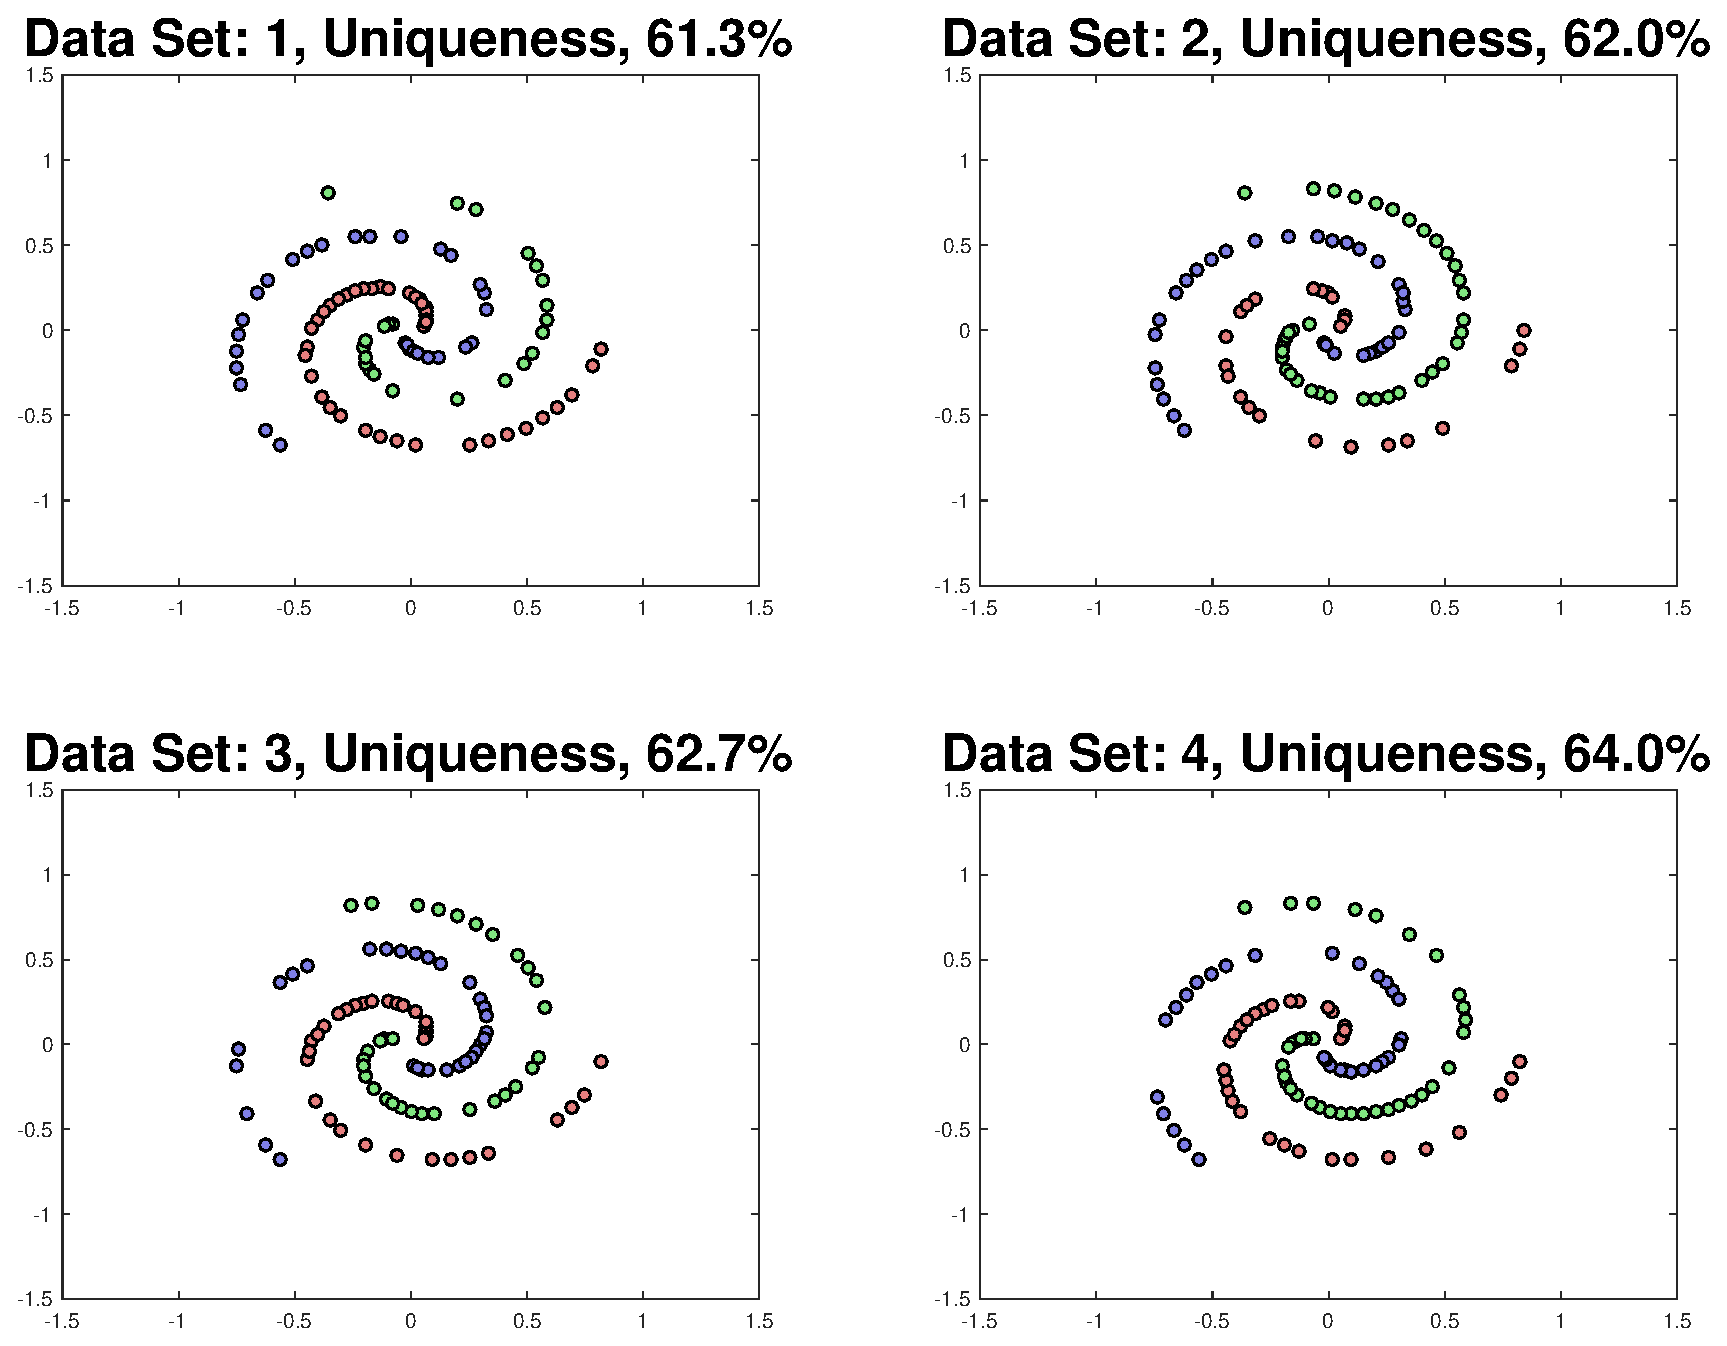
\includegraphics[width=0.60\columnwidth]{boot_strap}
    \caption{Overview of spectral subtraction process}
    \label{fig:boot_strap}
\end{figure}

The resulting data subsets sampled from the Toy Spiral data are shown in Figure \ref{fig:boot_strap}. Each dataset has 150 points however each spiral is not complete; some part of the spiral are missing. This is due to the fact that samples are drawn from the dataset with replacement. The amount of uniqueness in each dataset is presented in Figure \ref{fig:boot_strap} as well.  Ideally, as the size of our data set increases, the uniqueness percentage should approach $63.3\%$. The finite size of our dataset results in uniqueness values spread around the ideal. The table below shows the probability distributions of each class within the dataset. The roughly equal distributions corroborate the fact that sampling was performed uniformly.

\begin{table}[H]
\centering
\begin{tabular}{|c|c|}
\hline
Dataset Index & Class Probabilitites 		\\ \hline
1             & $[0.3733, 0.2733, 0.3533]$  	\\ \hline
2             & $[0.2800, 0.3667, 0.3533]$  	\\ \hline
3             & $[0.3333, 0.3200, 0.3467]$ 	\\ \hline
4             & $[0.3467, 0.3133, 0.3400]$  	\\ \hline
\end{tabular}
\end{table}

\subsection{Split Function}

The first step in the training of the decision forest is to develop the weak-learner functions that will be used to split the data at each node of the tree. Multiple weak-learner functions were implemented, namely axis-aligned and two-pixel. Linear, quadratic and cubic split functions were also implemented. Note that for the quadratic and cubic split functions have the form expressed in (\ref{eq:quad_split}) and (\ref{eq:cubic_split}) respectively.

\begin{align}
h(\textbf{v}, \theta) = [&a_1x_1^2+a_2x_2^2+a_3x_1x_2+a_4x_1+a_5x_2>\tau] \label{eq:quad_split} \\
h(\textbf{v}, \theta) = [&a_1x_1^3+a_2x_2^3+a_3x_1^2x_2+a_4x_1x_2^2+a_5x_1^2 \nonumber\\
&+a_6x_2^2+a_7x_1x_2+a_8x_1+a_9x_2>\tau] \label{eq:cubic_split}
\end{align}

The graphs below show the results obtained for all the weak-leaners tested, except for the two-pixel test. The two-pixel test did not perform well when tested with the 2-dimensional toy spiral data. Notice that the graphs obtained show the results when \texttt{param.splitNum} was set at 3. The results are indicative of the fact that a stronger class of learner functions does not necessarily translate into a greater information gain when the number of split functions tested is small.

\begin{figure}[H]
	\centering
    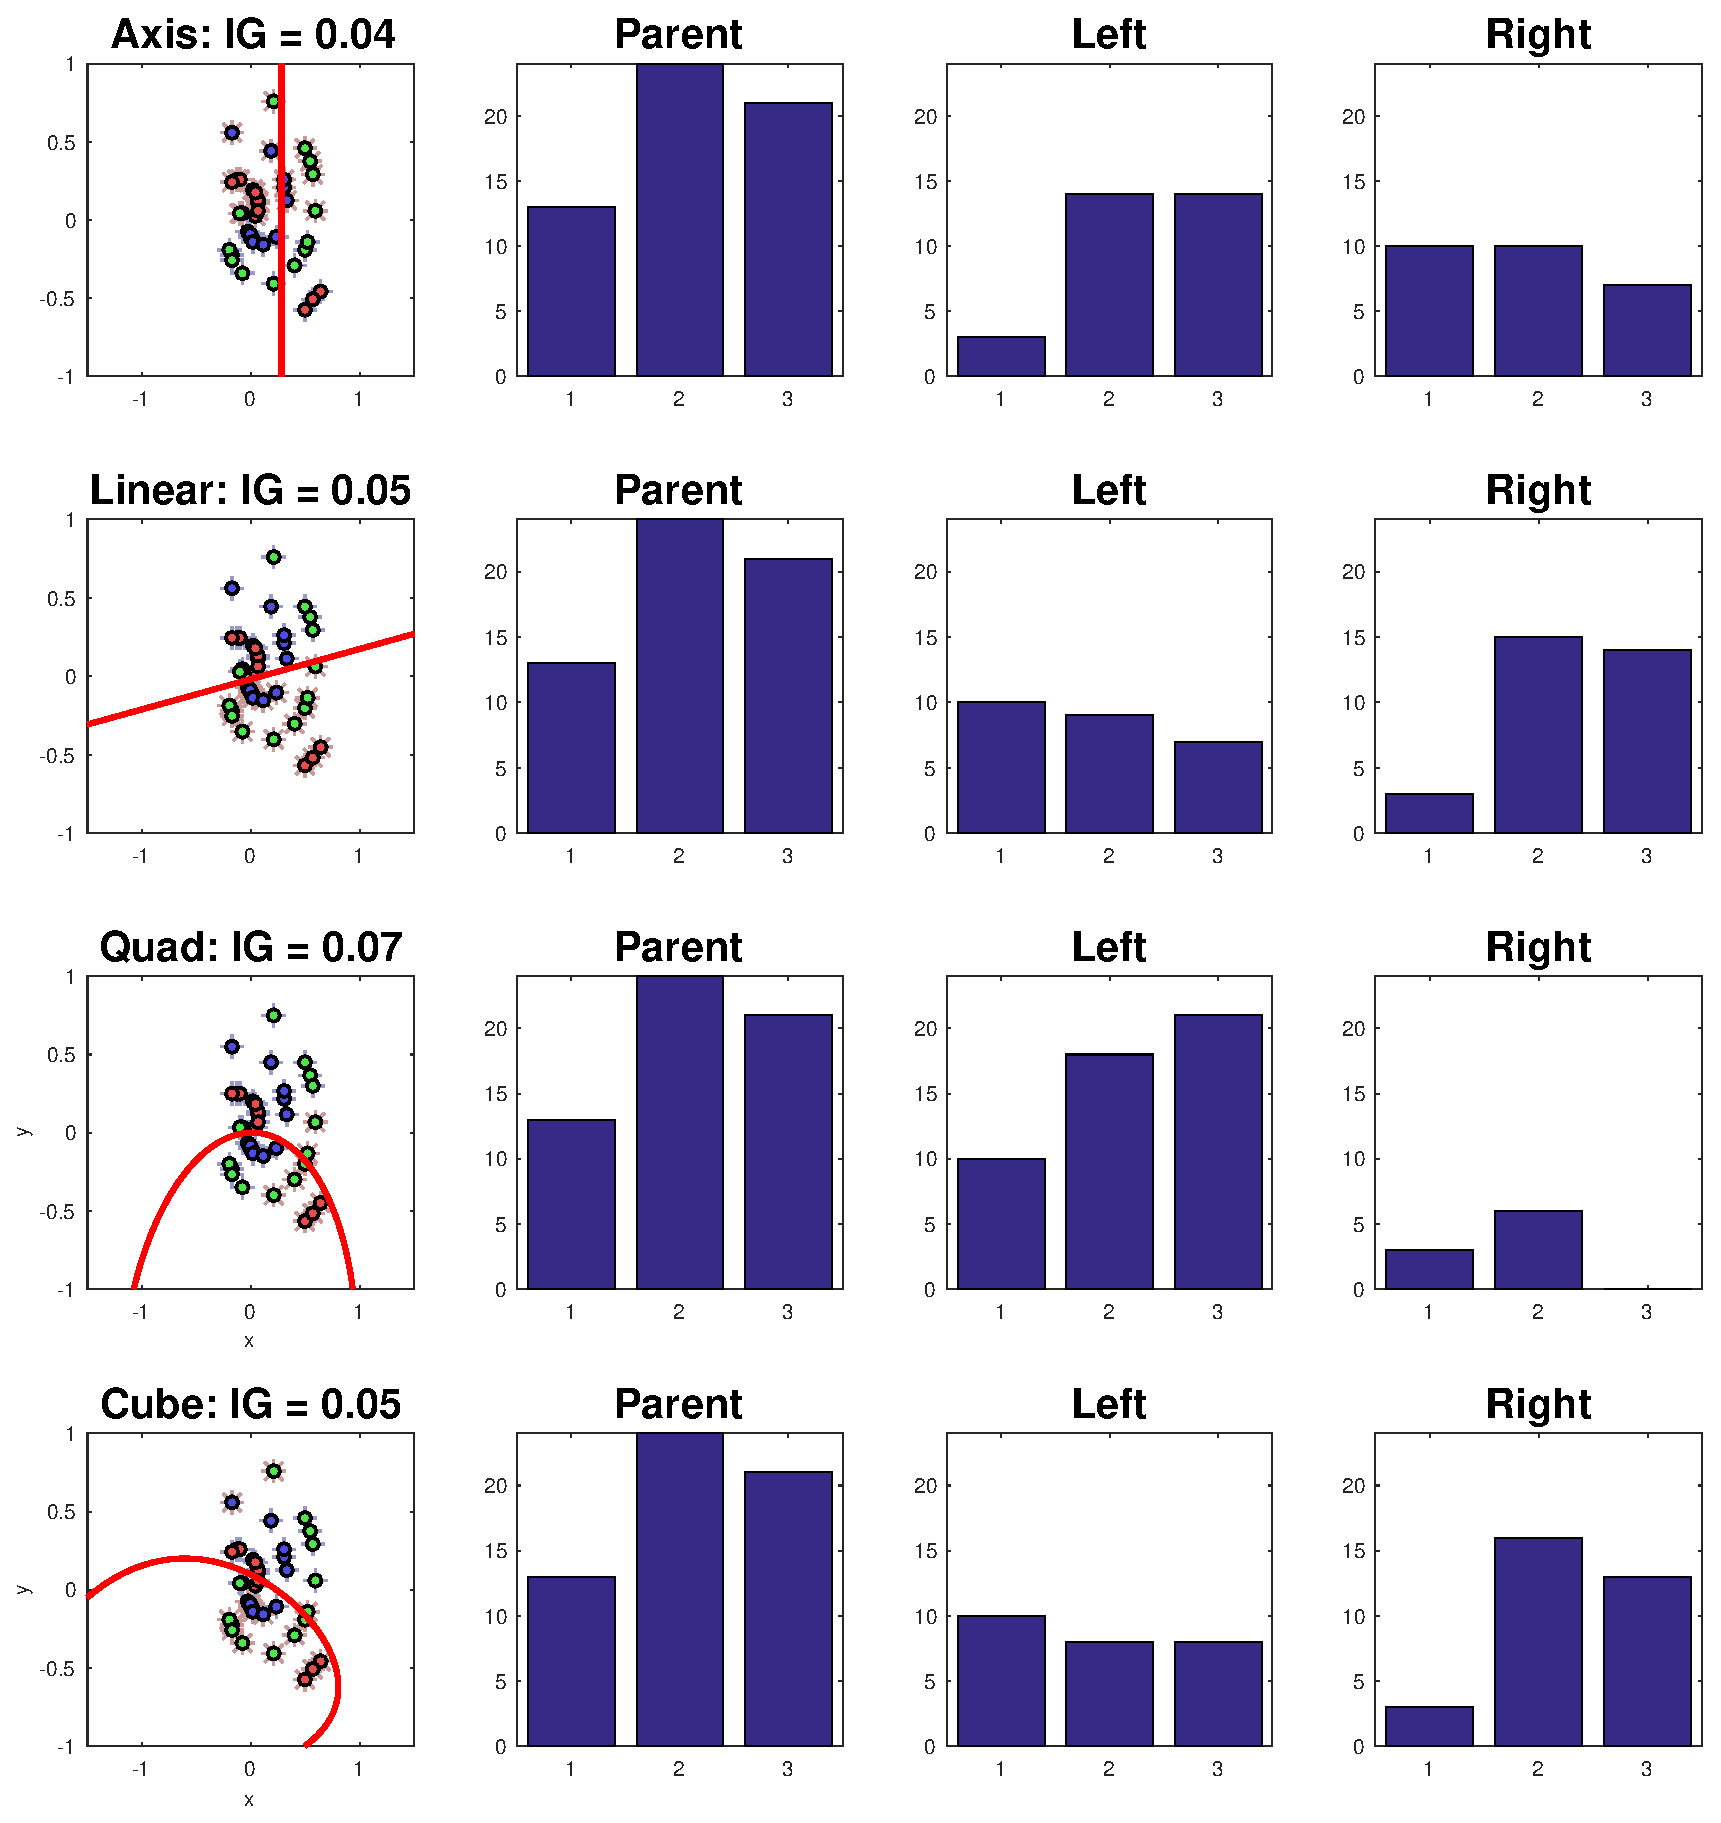
\includegraphics[width=0.60\columnwidth]{split_function_visualitions_1}
    \caption{Overview of spectral subtraction process}
    \label{fig:learners_1}
\end{figure}

The graph in Figure \ref{fig:learners_2} shows the effects that the strength of the learning class has when tested on nodes with a small number of data points. Observe the split function obtained for the quadratic and cubic learners. \textbf{There is clear over-fitting of the data.} This is completely in line with the results obtained from Vapnik–Chervonenkis theory. Quadratic and Cubic functions have a greater Vapnik–Chervonenkis (VC) dimension and trained on a small number of points, these learners will overfit data not generalize well. The random forest algorithm provides a mechanism, the committee machine, to combat over-fitting in each individual tree. As such, in the next section, it should be noted that if strong non-linear learners are used, the number of trees should also be increased to achieve the same performance as a weak learner. 

\begin{figure}[H]
	\centering
    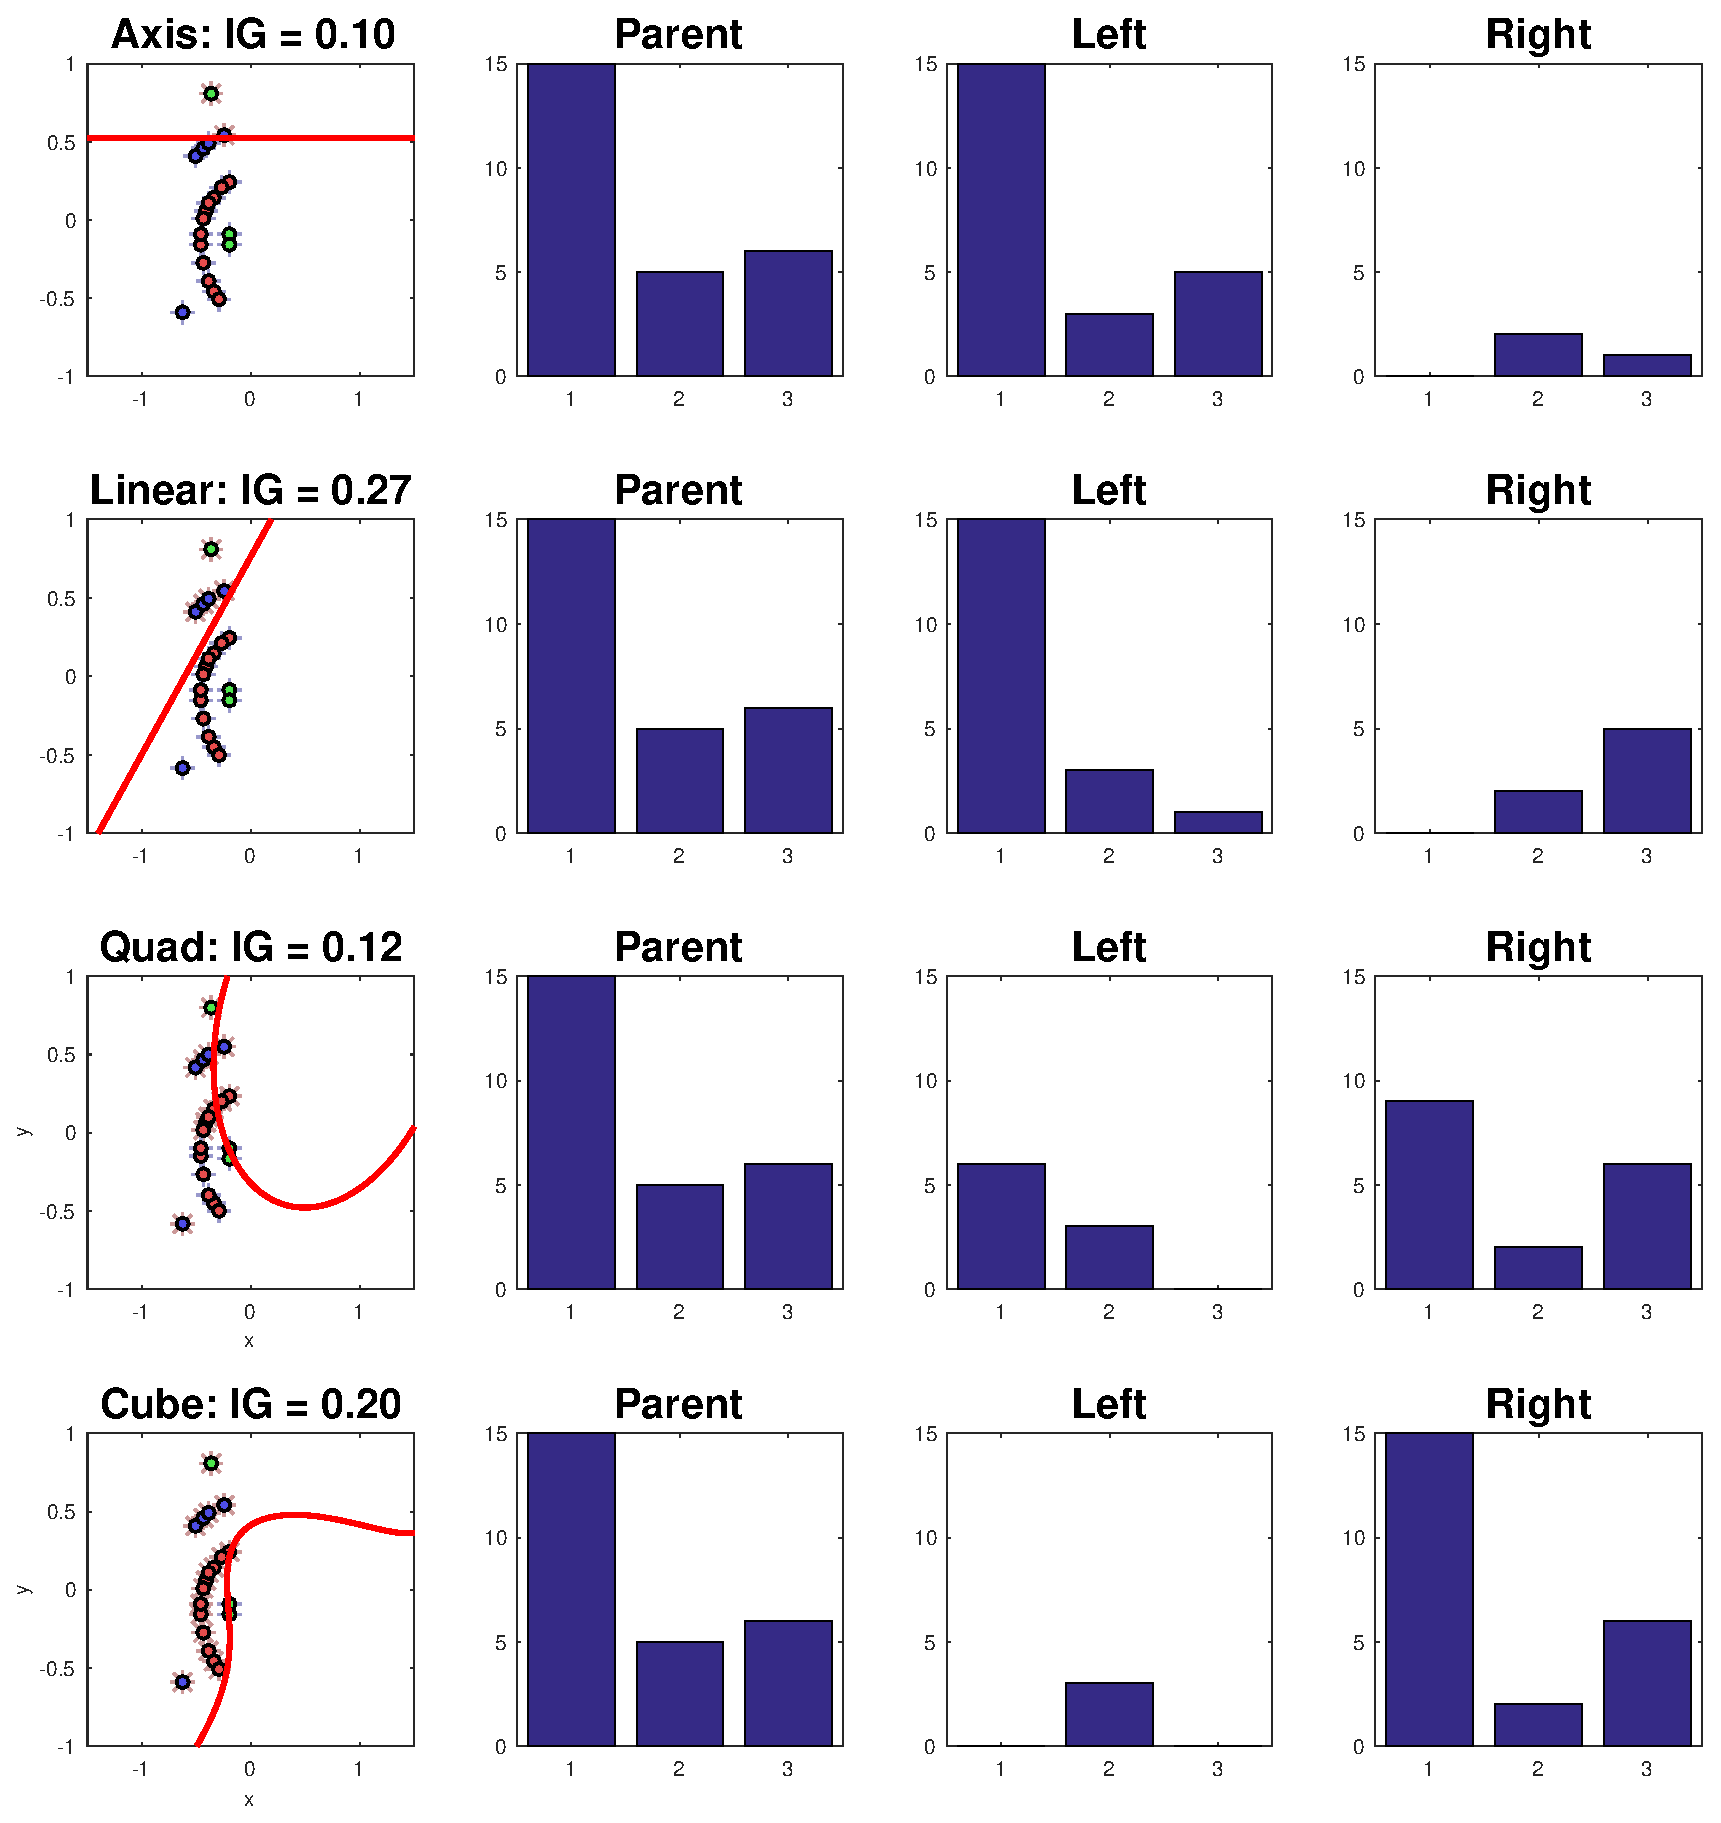
\includegraphics[width=0.60\columnwidth]{split_function_visualitions_3}
    \caption{Overview of spectral subtraction process}
    \label{fig:learners_2}
\end{figure}

By simply analyzing Figure \ref{fig:learners_1} and \ref{fig:learners_2}, we clearly see the advantages of using a stronger learning class. For this, we have to set \texttt{param.splitNum} to 20. Figure \ref{fig:learners_3} makes it clear that stronger learning classes are able to split the data more efficiently and obtain a higher information gain. The discriminating power of the learning classes is not obvious when the number of split functions tested is small however increasing \texttt{param.splitNum} clearly highlights the each classes discriminating power. 

\begin{figure}[H]
	\centering
    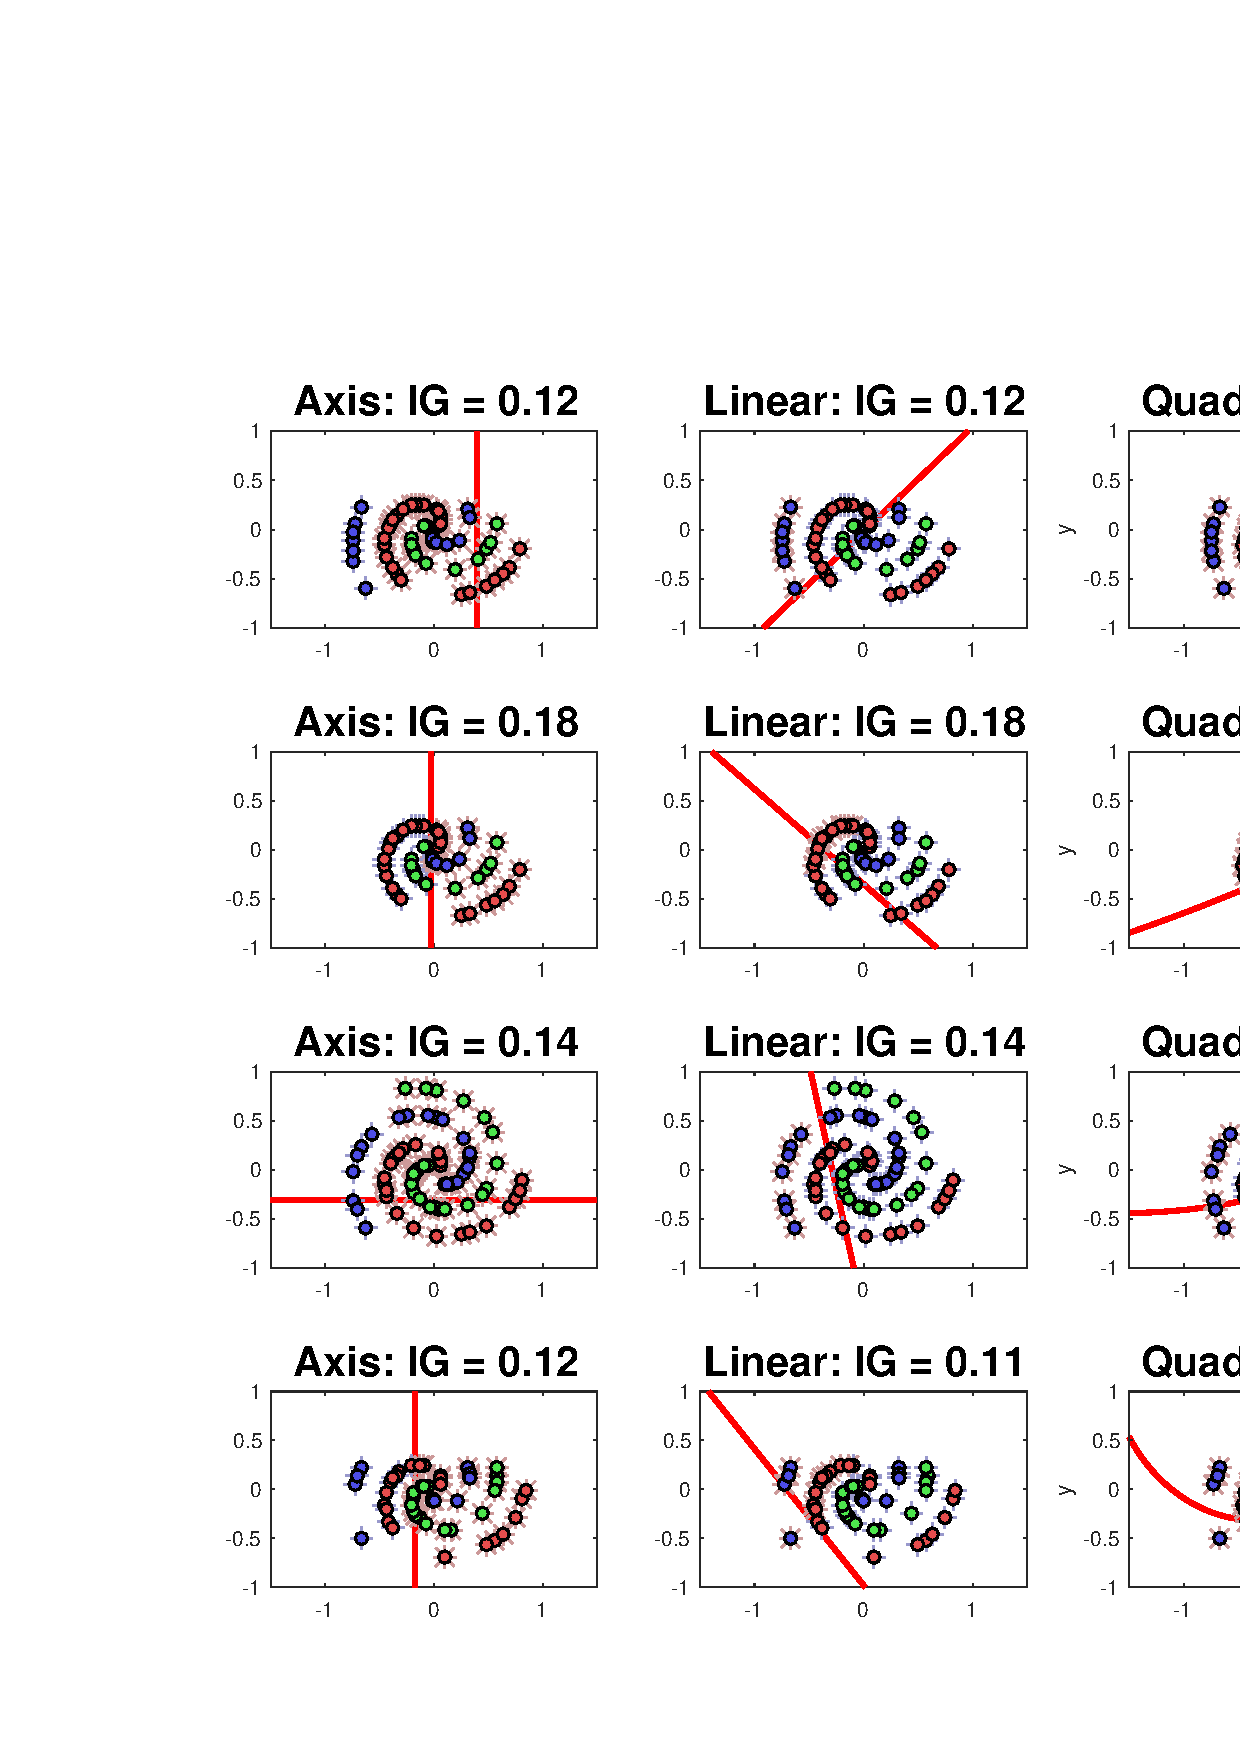
\includegraphics[width=0.60\columnwidth]{split_function_visualitions_5}
    \caption{Overview of spectral subtraction process}
    \label{fig:learners_3}
\end{figure}

Using a stronger learning class such as the quadratic or cubic non-linear functions has it benefits. They do lead to an increased information gain at each node. However, the increasing the strength of the learning class should also be accompanied with a small increase in the number of split functions tested. Stronger class have more degrees of freedom and thus search for a linear separator in a higher dimensional space. As such, keeping the number of split functions that we test constant is not ideal.

\subsection{Growing Tree}
Lastly, the leaf nodes have been visualized in Figure \ref{fig:leaf_nodes}. The leaf nodes have been generated using the axis-aligned weak learner with \texttt{param.splitNum} set to 3. Most leaves contain only one class of data points; the recursive splitting of the data points down the tree has a distilling effect. There are some leaves with 2 or more classes of data. This can be attributed to the difficulty in splitting the region near the middle of the Toy Spiral where the data points are tightly clustered.

\begin{figure}[H]
	\centering
    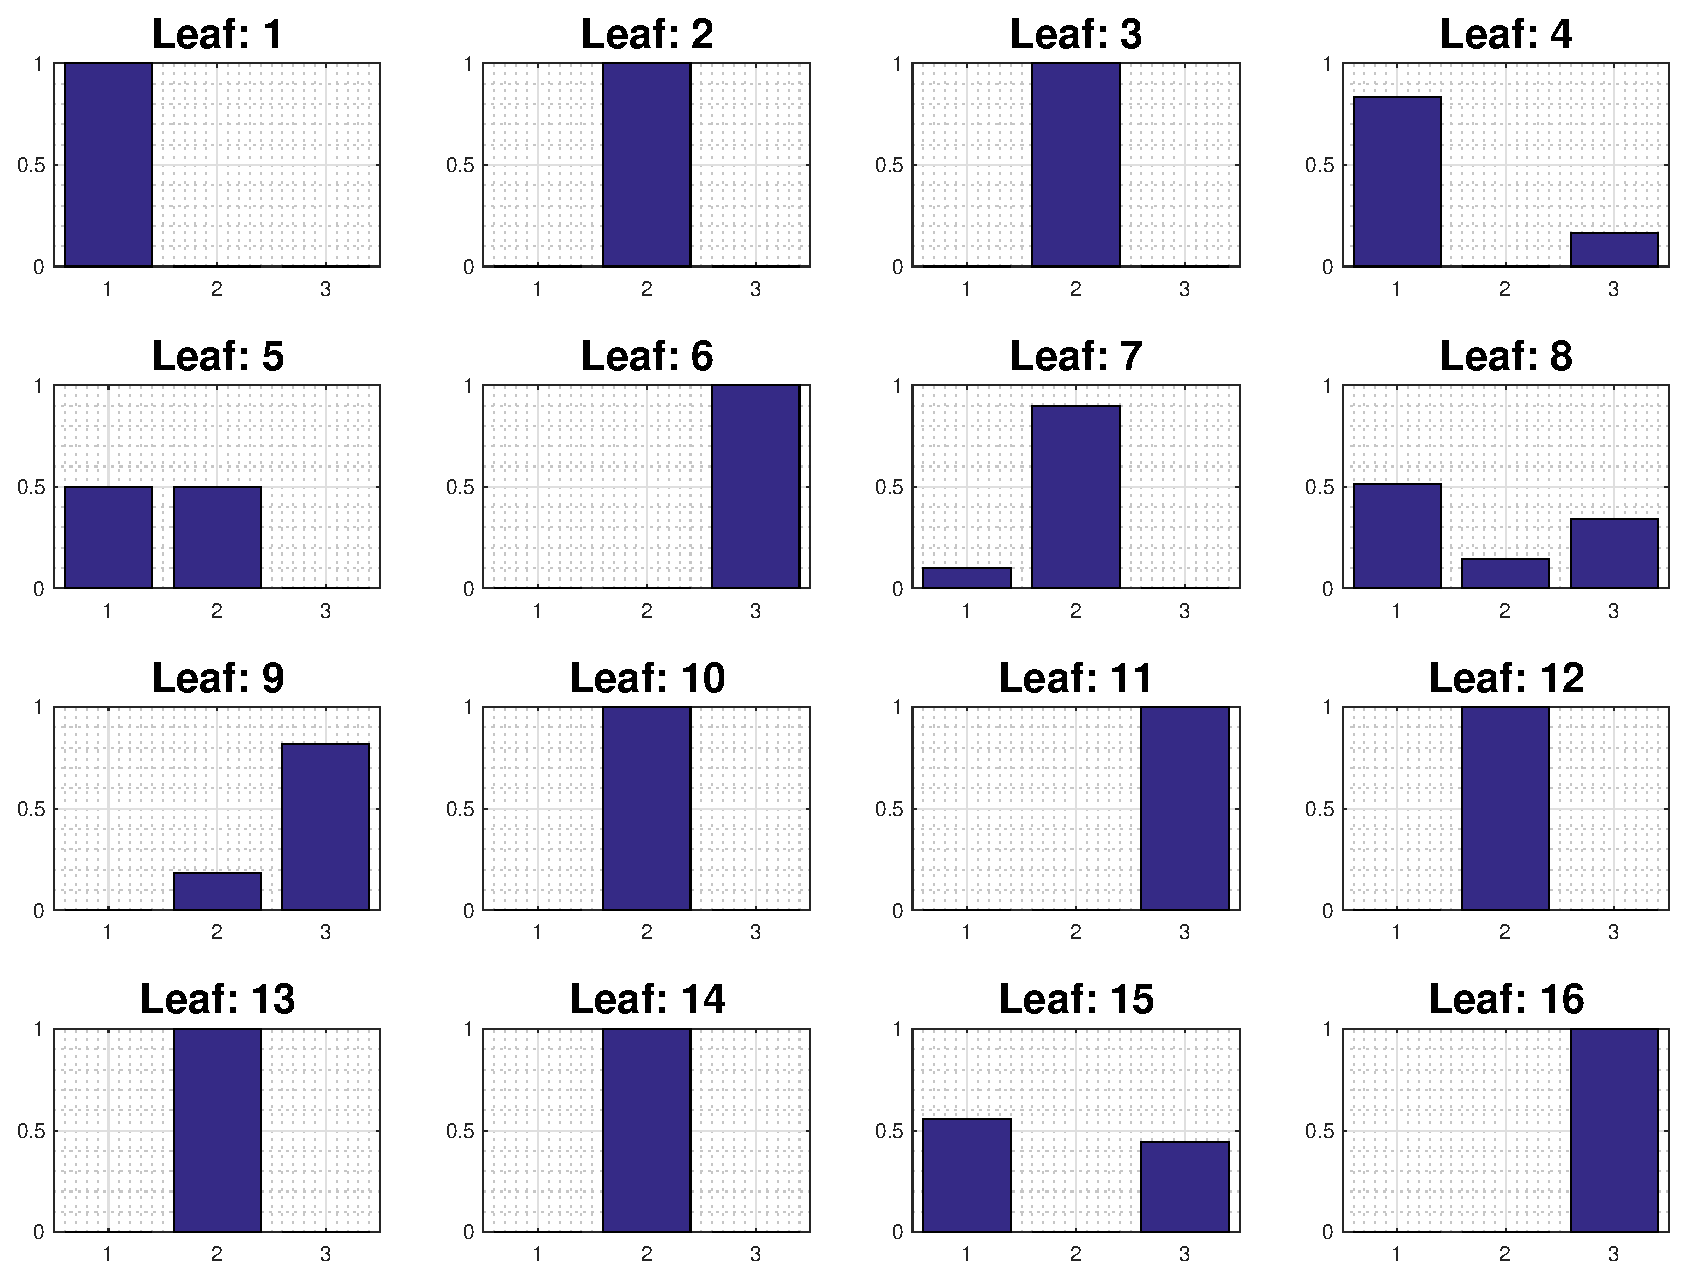
\includegraphics[width=0.60\columnwidth]{leaf_node_distributions_1}
    \caption{Overview of spectral subtraction process}
    \label{fig:leaf_nodes}
\end{figure}

The tree was built using two spotting criteria. Firstly, a node is considered a leaf if there are less 5 training points reach the node. The reason for this is because, training on such a limited number of points is not going to lead to good results. If only 5 points arrive at a node, they will be concentrated within a small region. Training based on these points will lead to over-fitting. The second stopping criteria is the maximum tree depth. This is simple to implement and gives us direct control on the maximum number of leaves. Using the tree-depth to control the number of leaves will come in handy when growing an random forest code-book.

\section{Evaluating Decision Forest}

The 4 test points are evaluated on a forest containing 3 trees; the results obtained are graphed below. The histograms show the probability distribution functions at each leaf for each point. The averaged values have also been plotted. Note that test point 1 (-0.5, -0.7), has been mis-classified; ideally, the point should be blue. The reasons for this misclassification is multi-fold. One of the main factors is that he random forest currently only have 3 trees and thus the averaging effect of the committee machine is limited.

\begin{figure}[H]
	\centering
    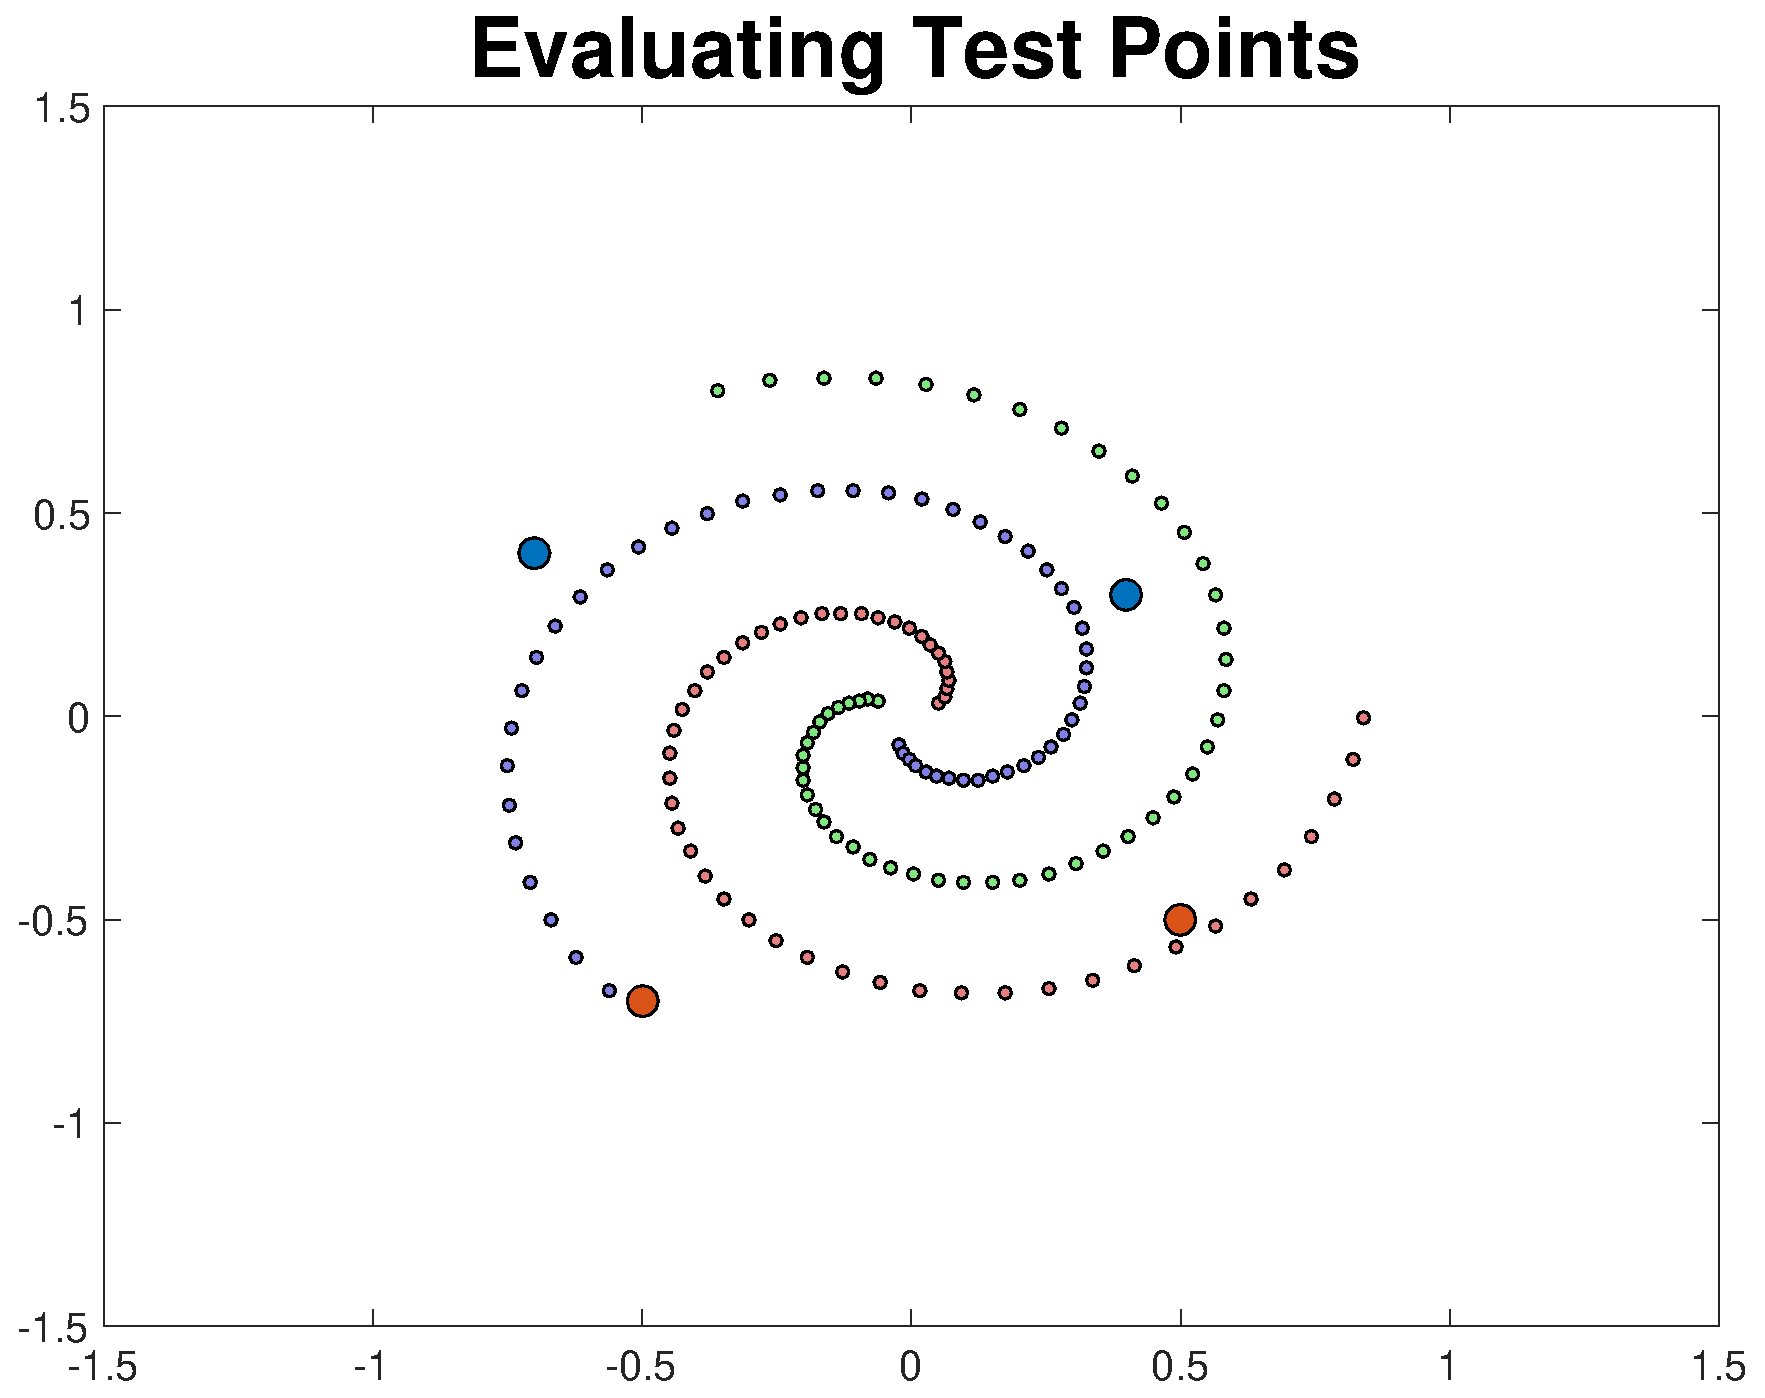
\includegraphics[width=0.49\columnwidth]{test_points_eval}
    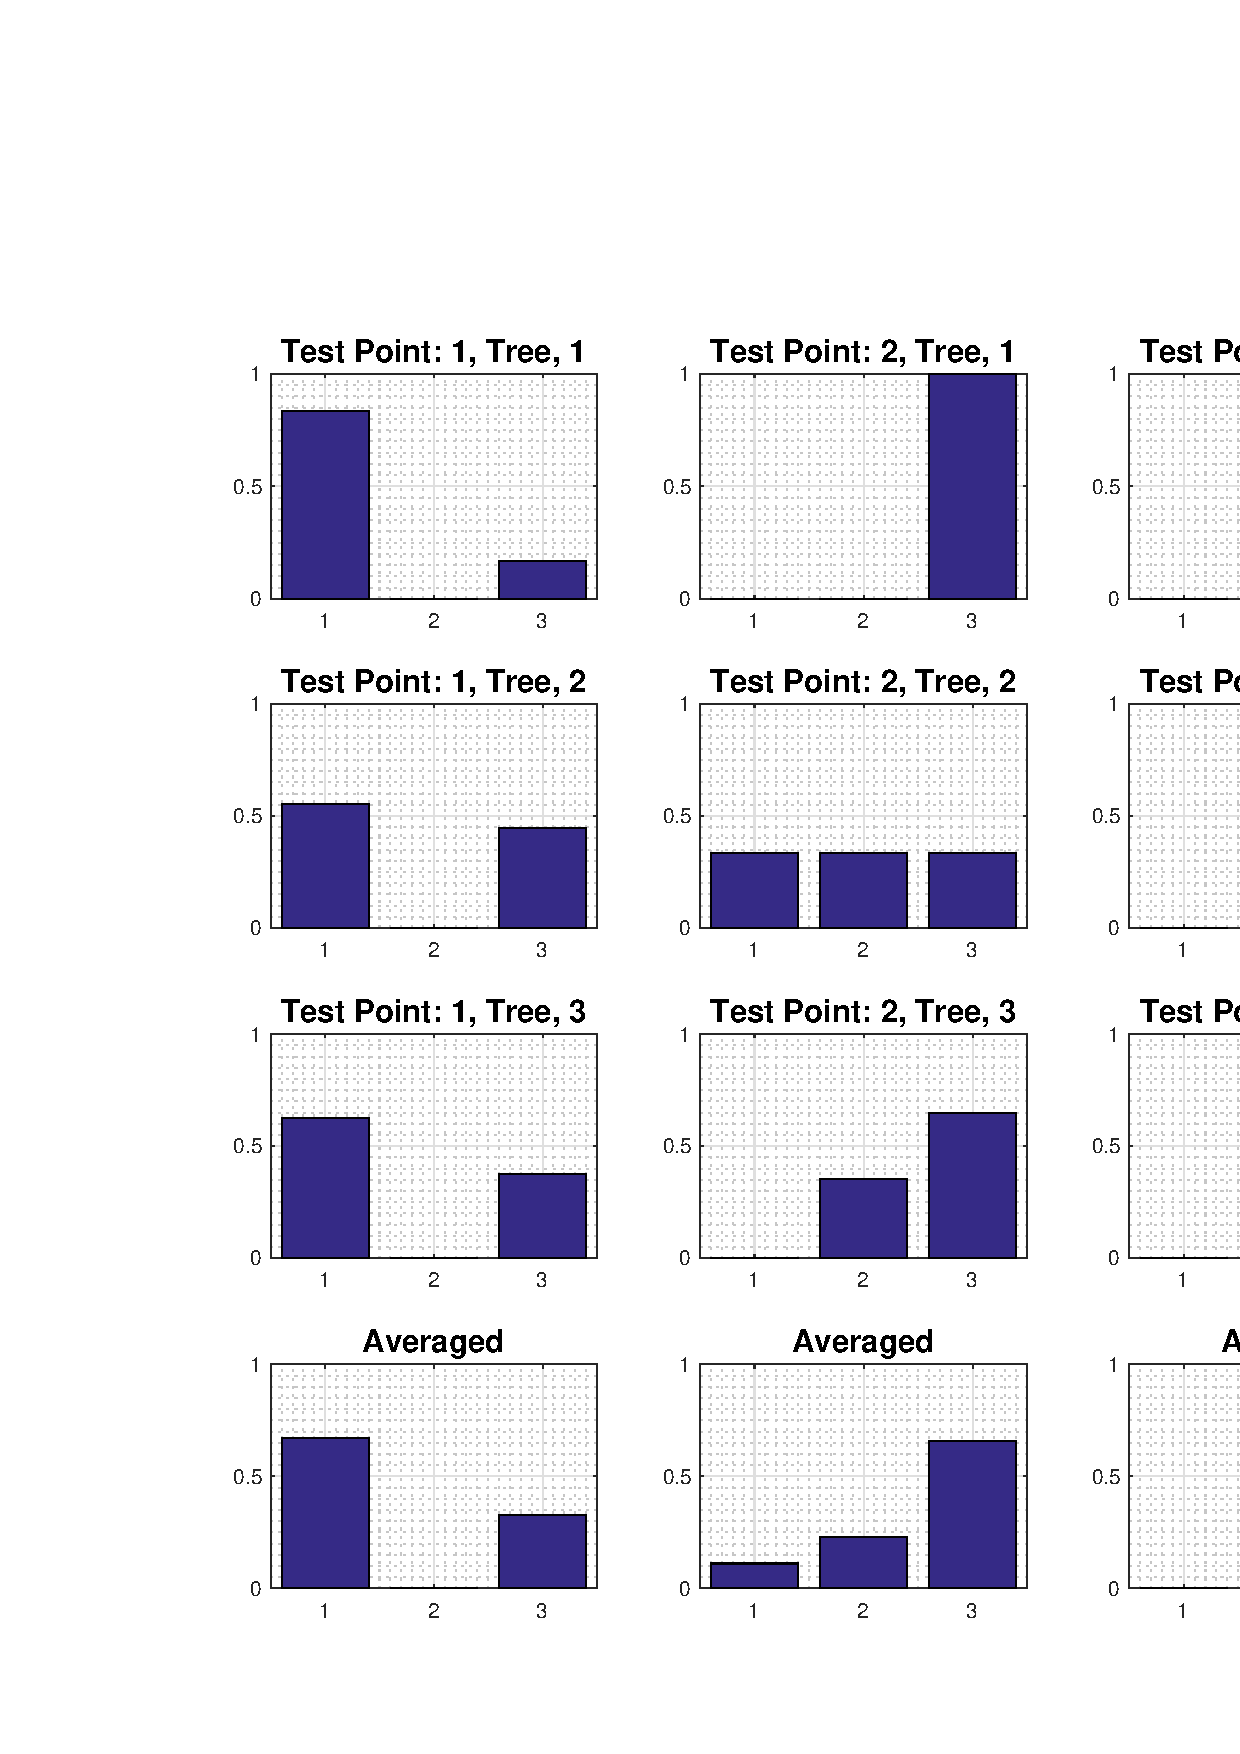
\includegraphics[width=0.49\columnwidth]{test_points_hist}
    \caption{Overview of spectral subtraction process}
    \label{fig:leaf_nodes}
\end{figure}

\subsection{Varying Number of Trees}

To directly combat the misclassification observed above, the first parameter that is varied is the number of trees in the forest. The graph below shows that increasing the number of trees has a considerable effect on the classification process, when the absolute number of trees is small. Increasing the number of tress from 100 to 200 has negligible effect. Notice the straight axis-aligned class boundaries obtained in the region of the grid for which extrapolation is required. Training data is contained within the unit square whereas the region for which the classifier is tested extends beyond the unit square. The classifier is expected to extrapolate the class boundaries. Since the axis-aligned weak learner is used, the extrapolation leads to straight axis-aligned lines in the extrapolated region. 

\begin{figure}[H]
	\centering
    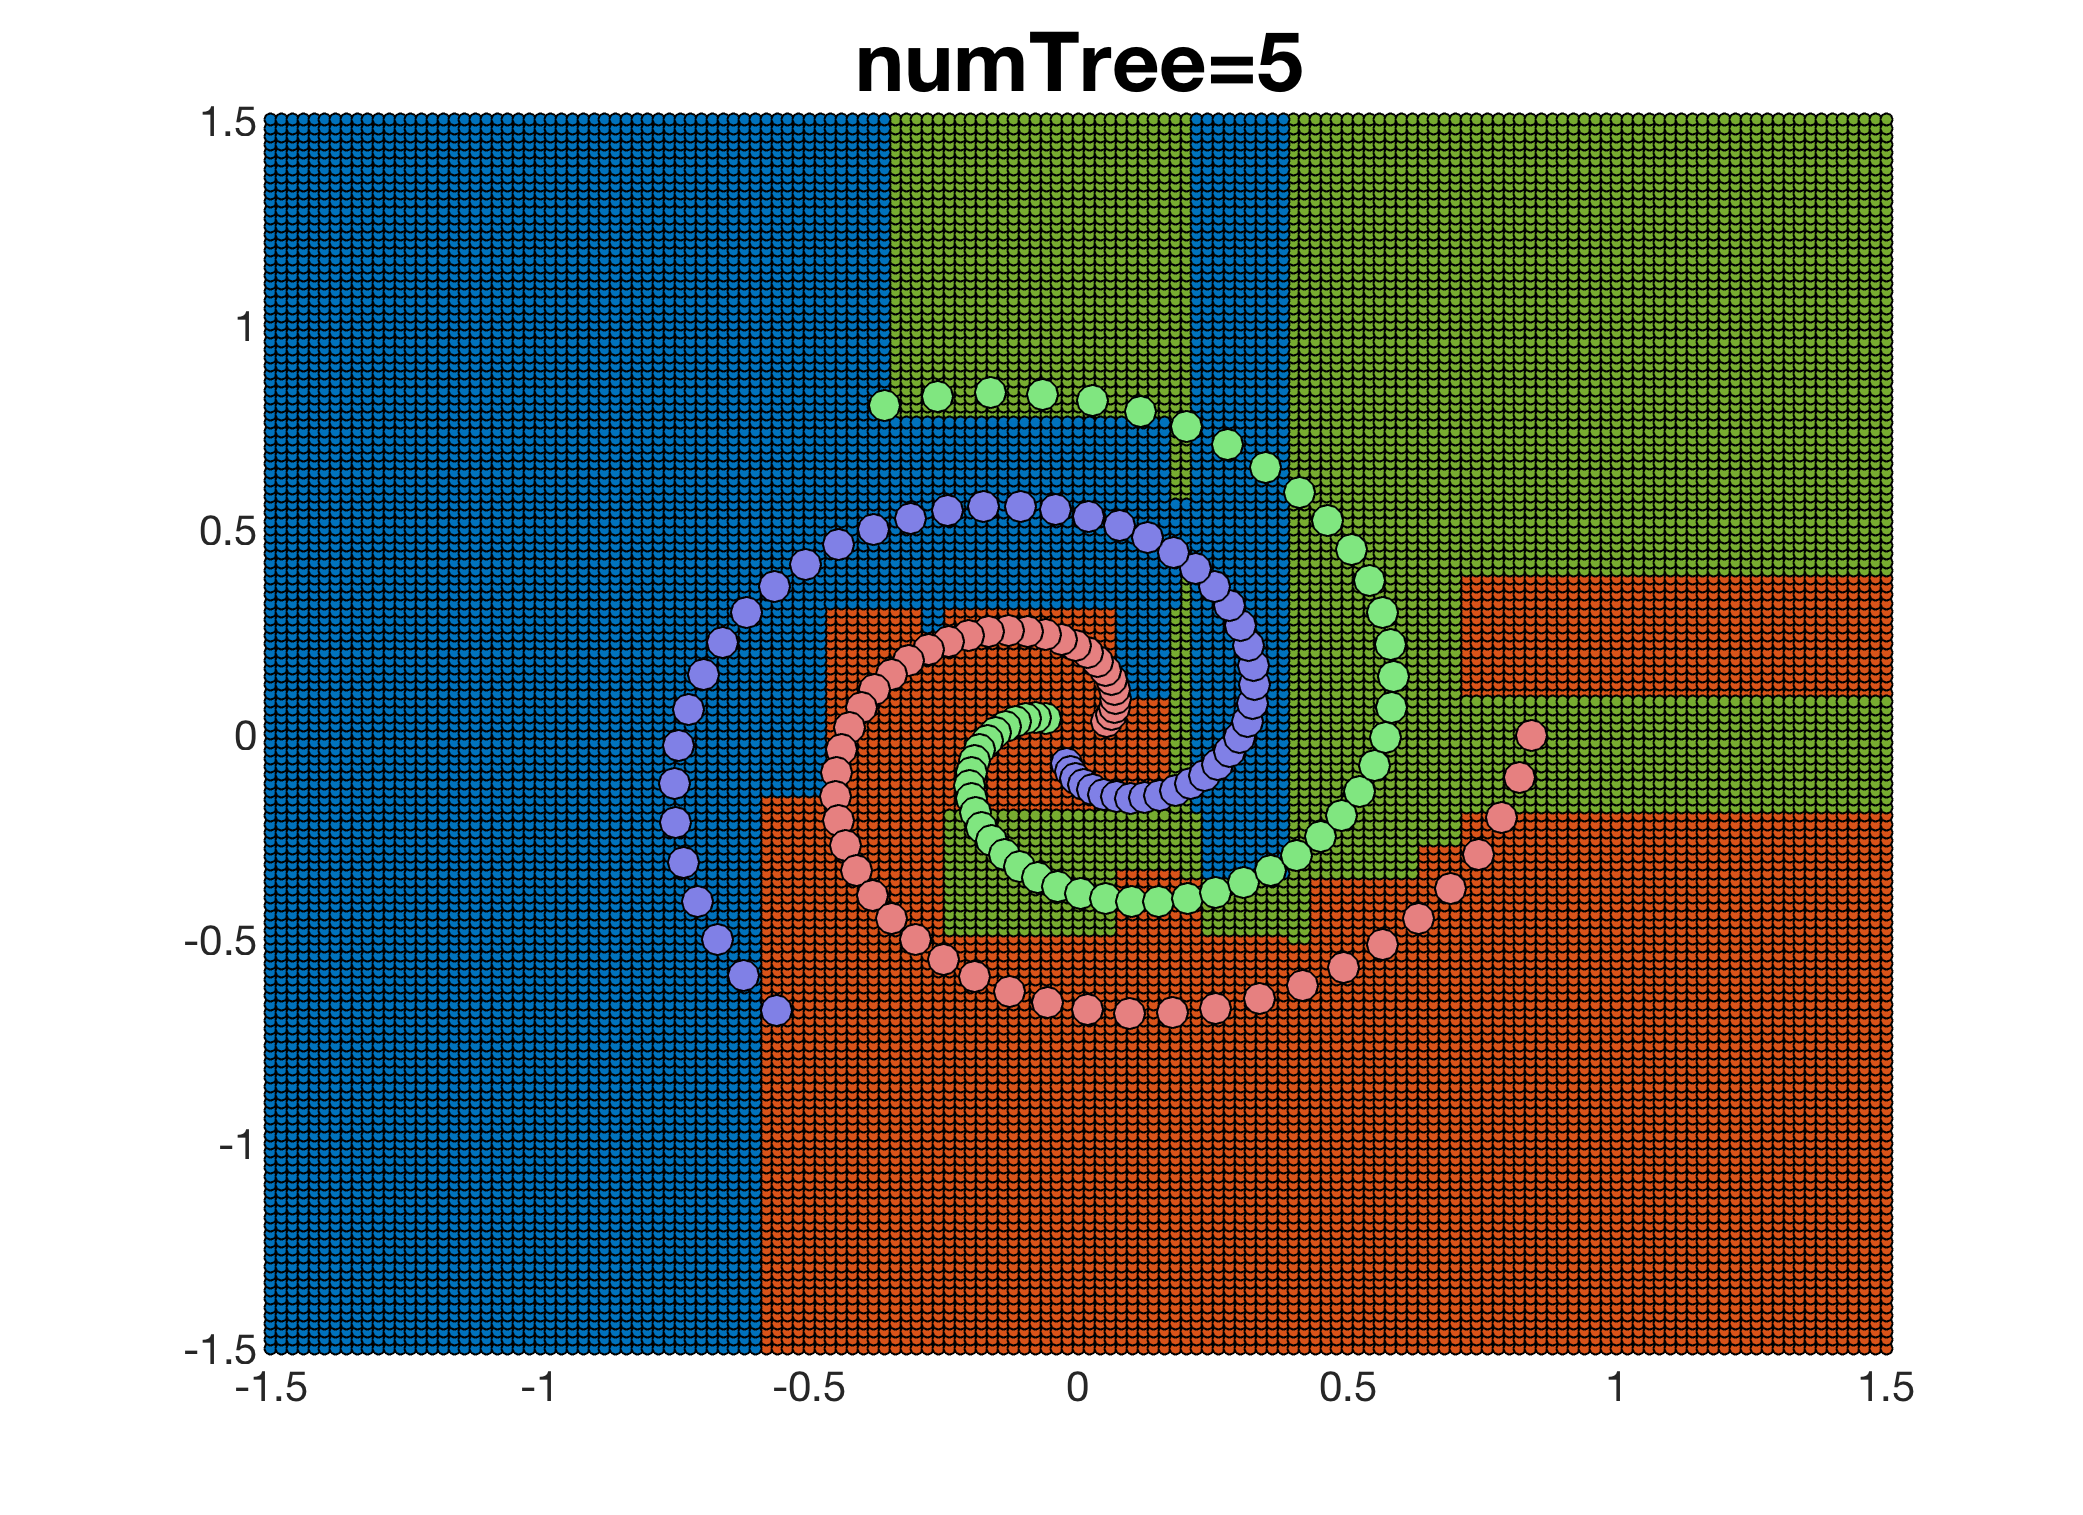
\includegraphics[width=0.40\columnwidth]{ax_5_trees}
	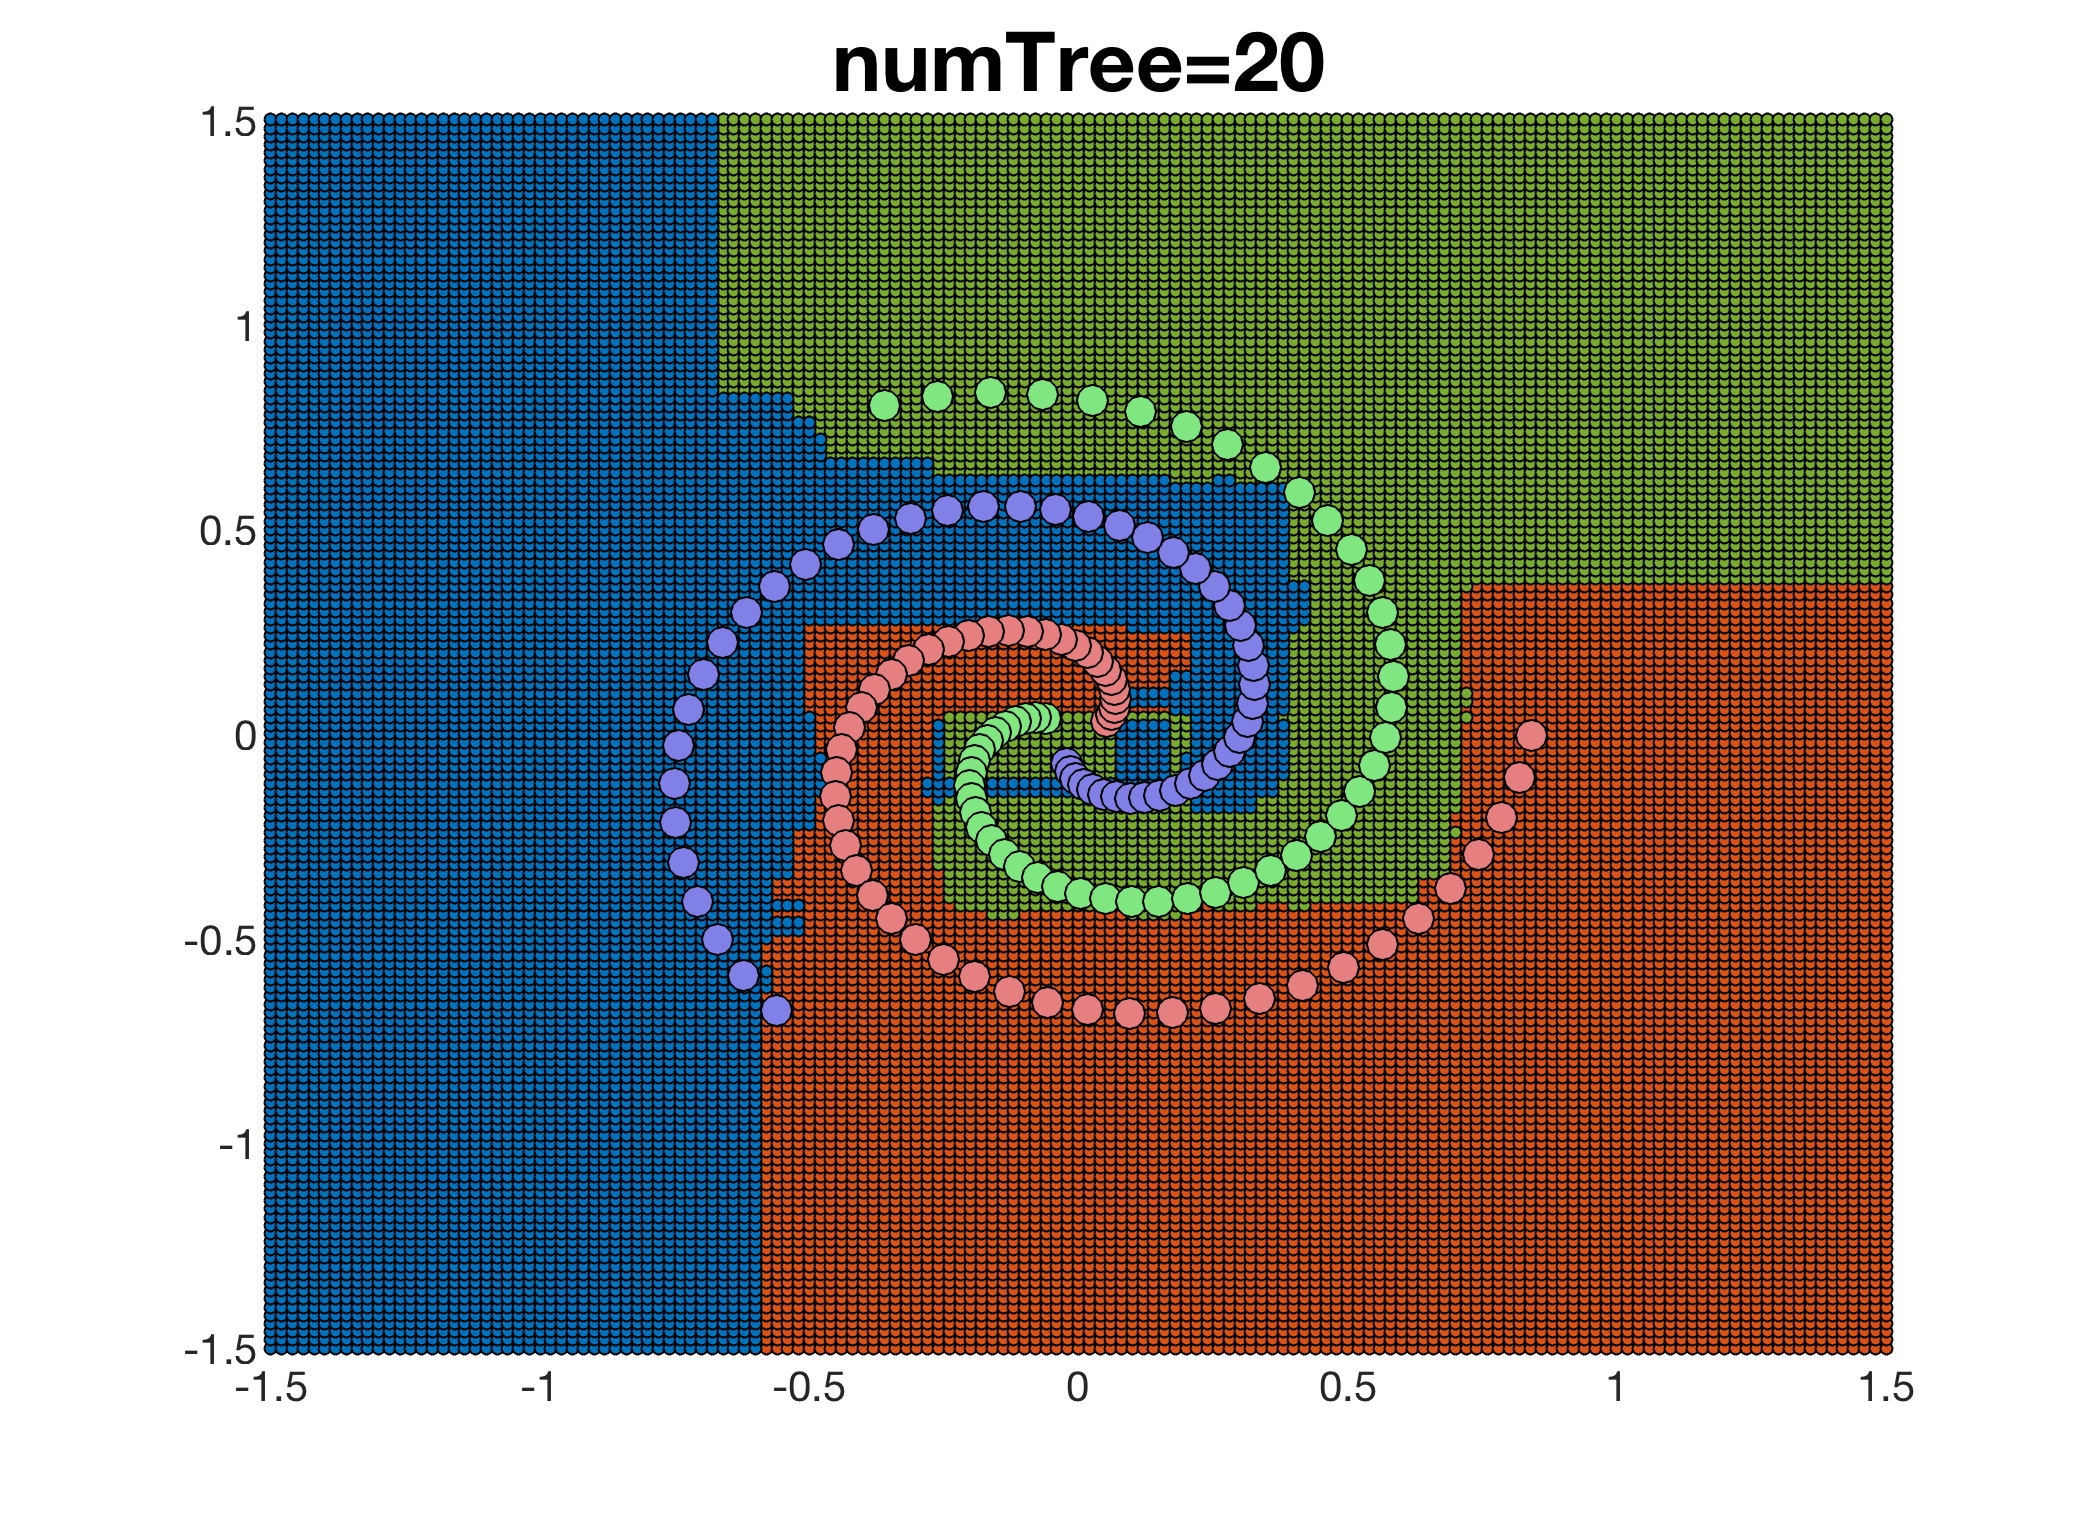
\includegraphics[width=0.40\columnwidth]{ax_20_trees}
    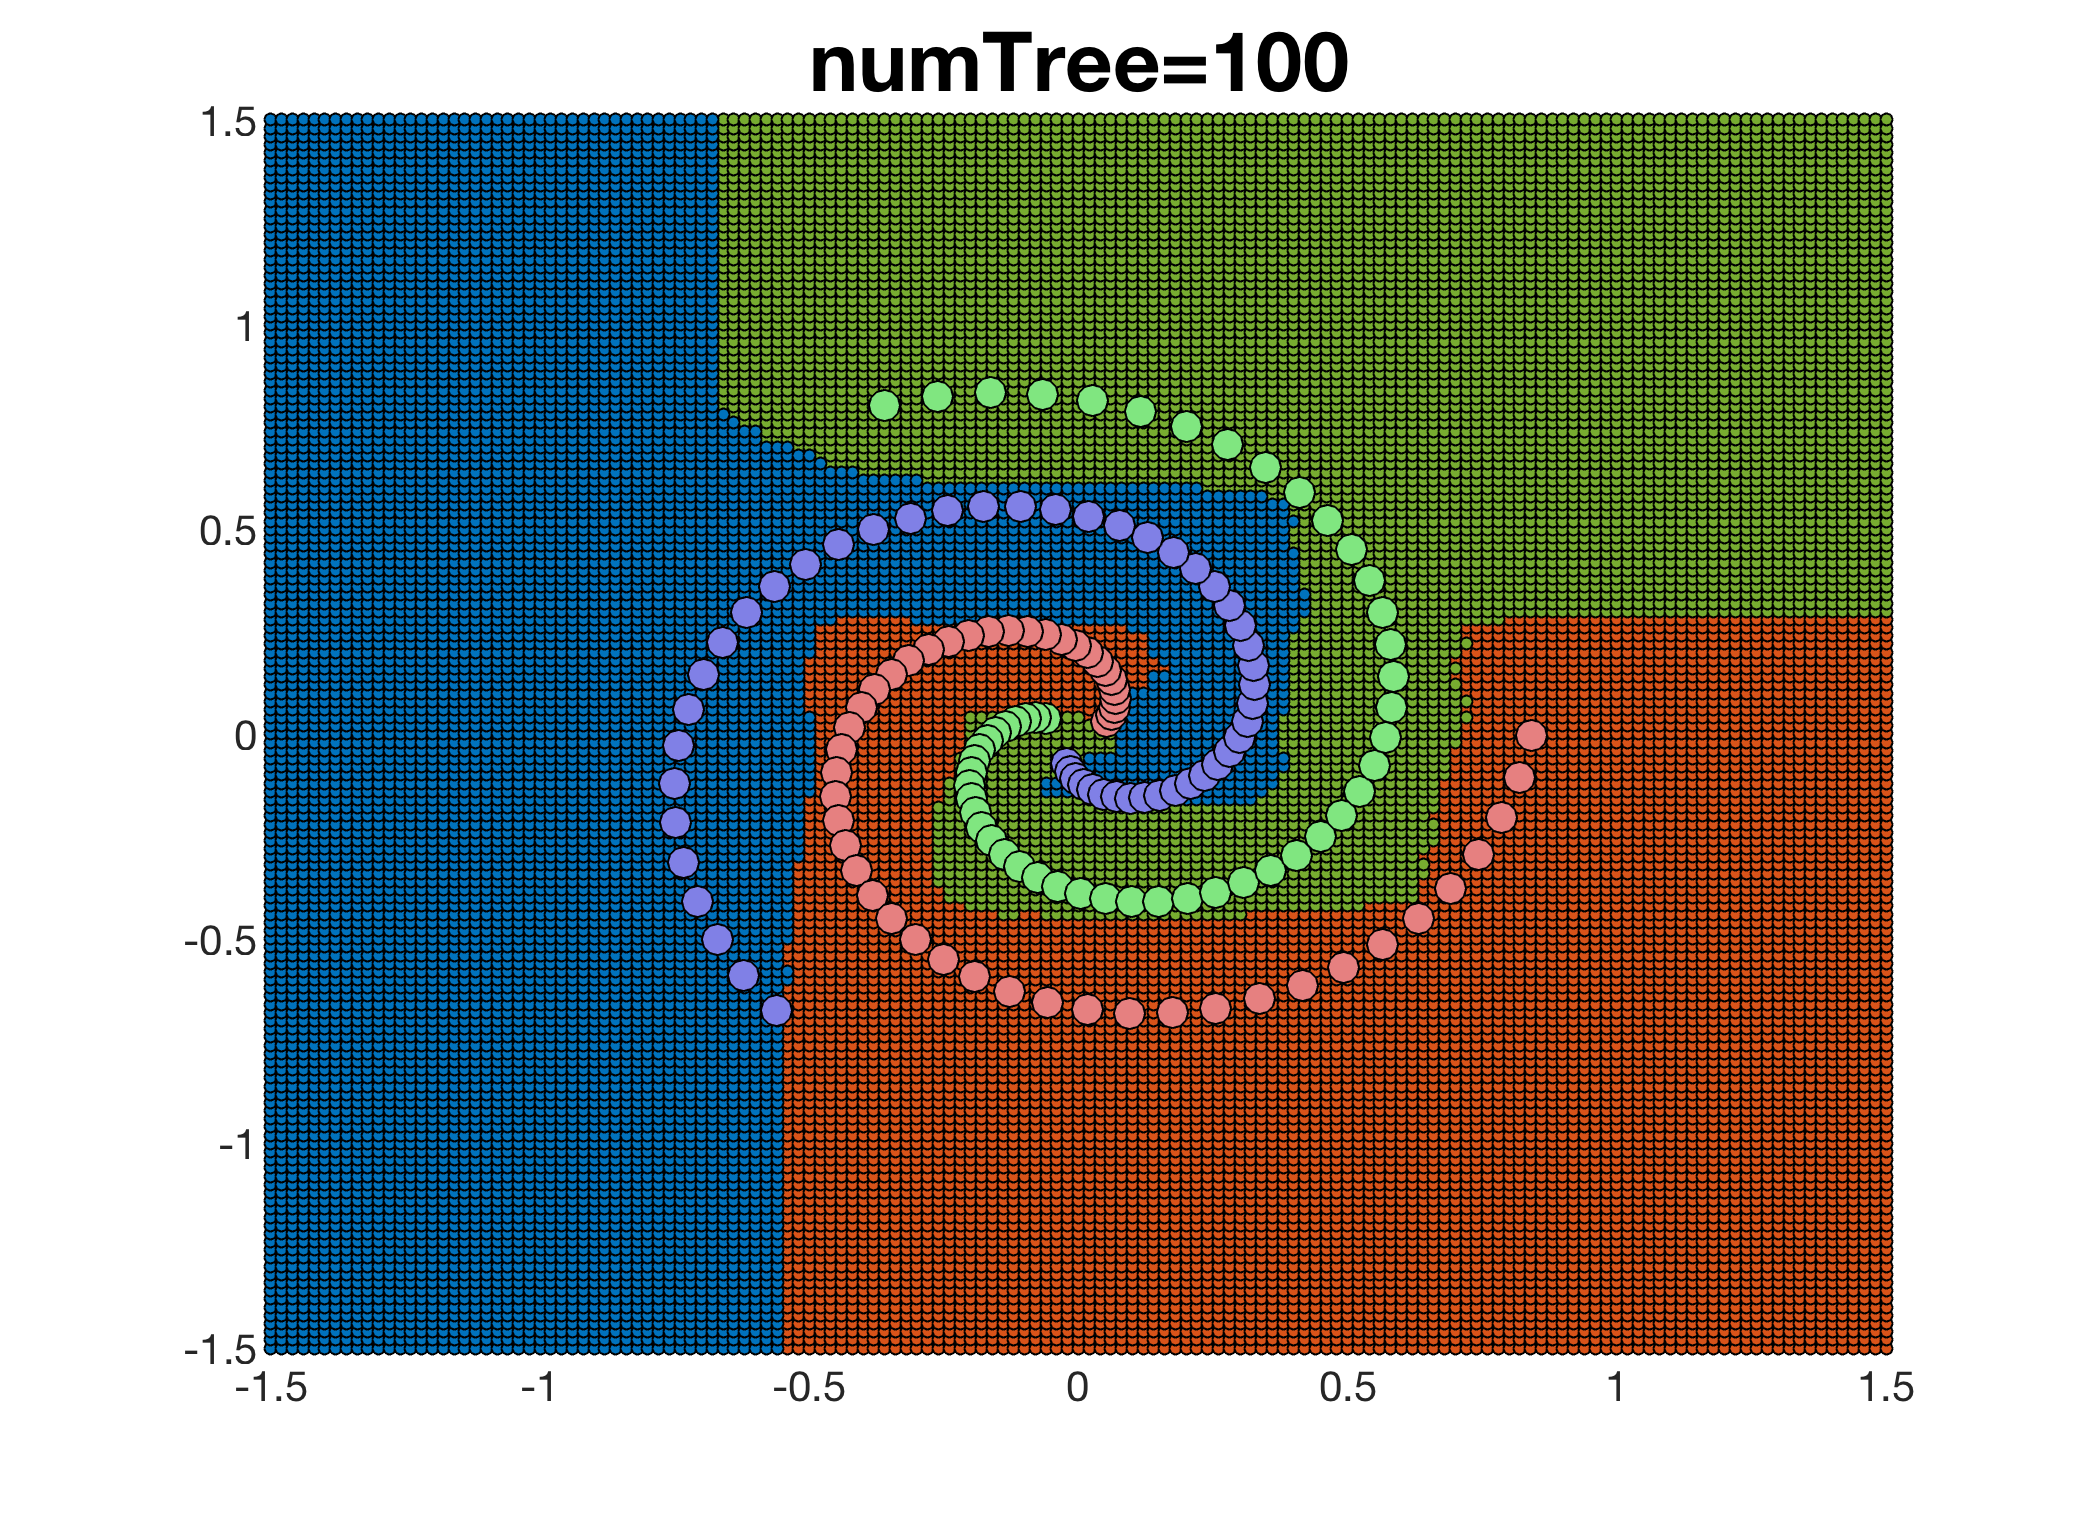
\includegraphics[width=0.40\columnwidth]{ax_100_trees}
    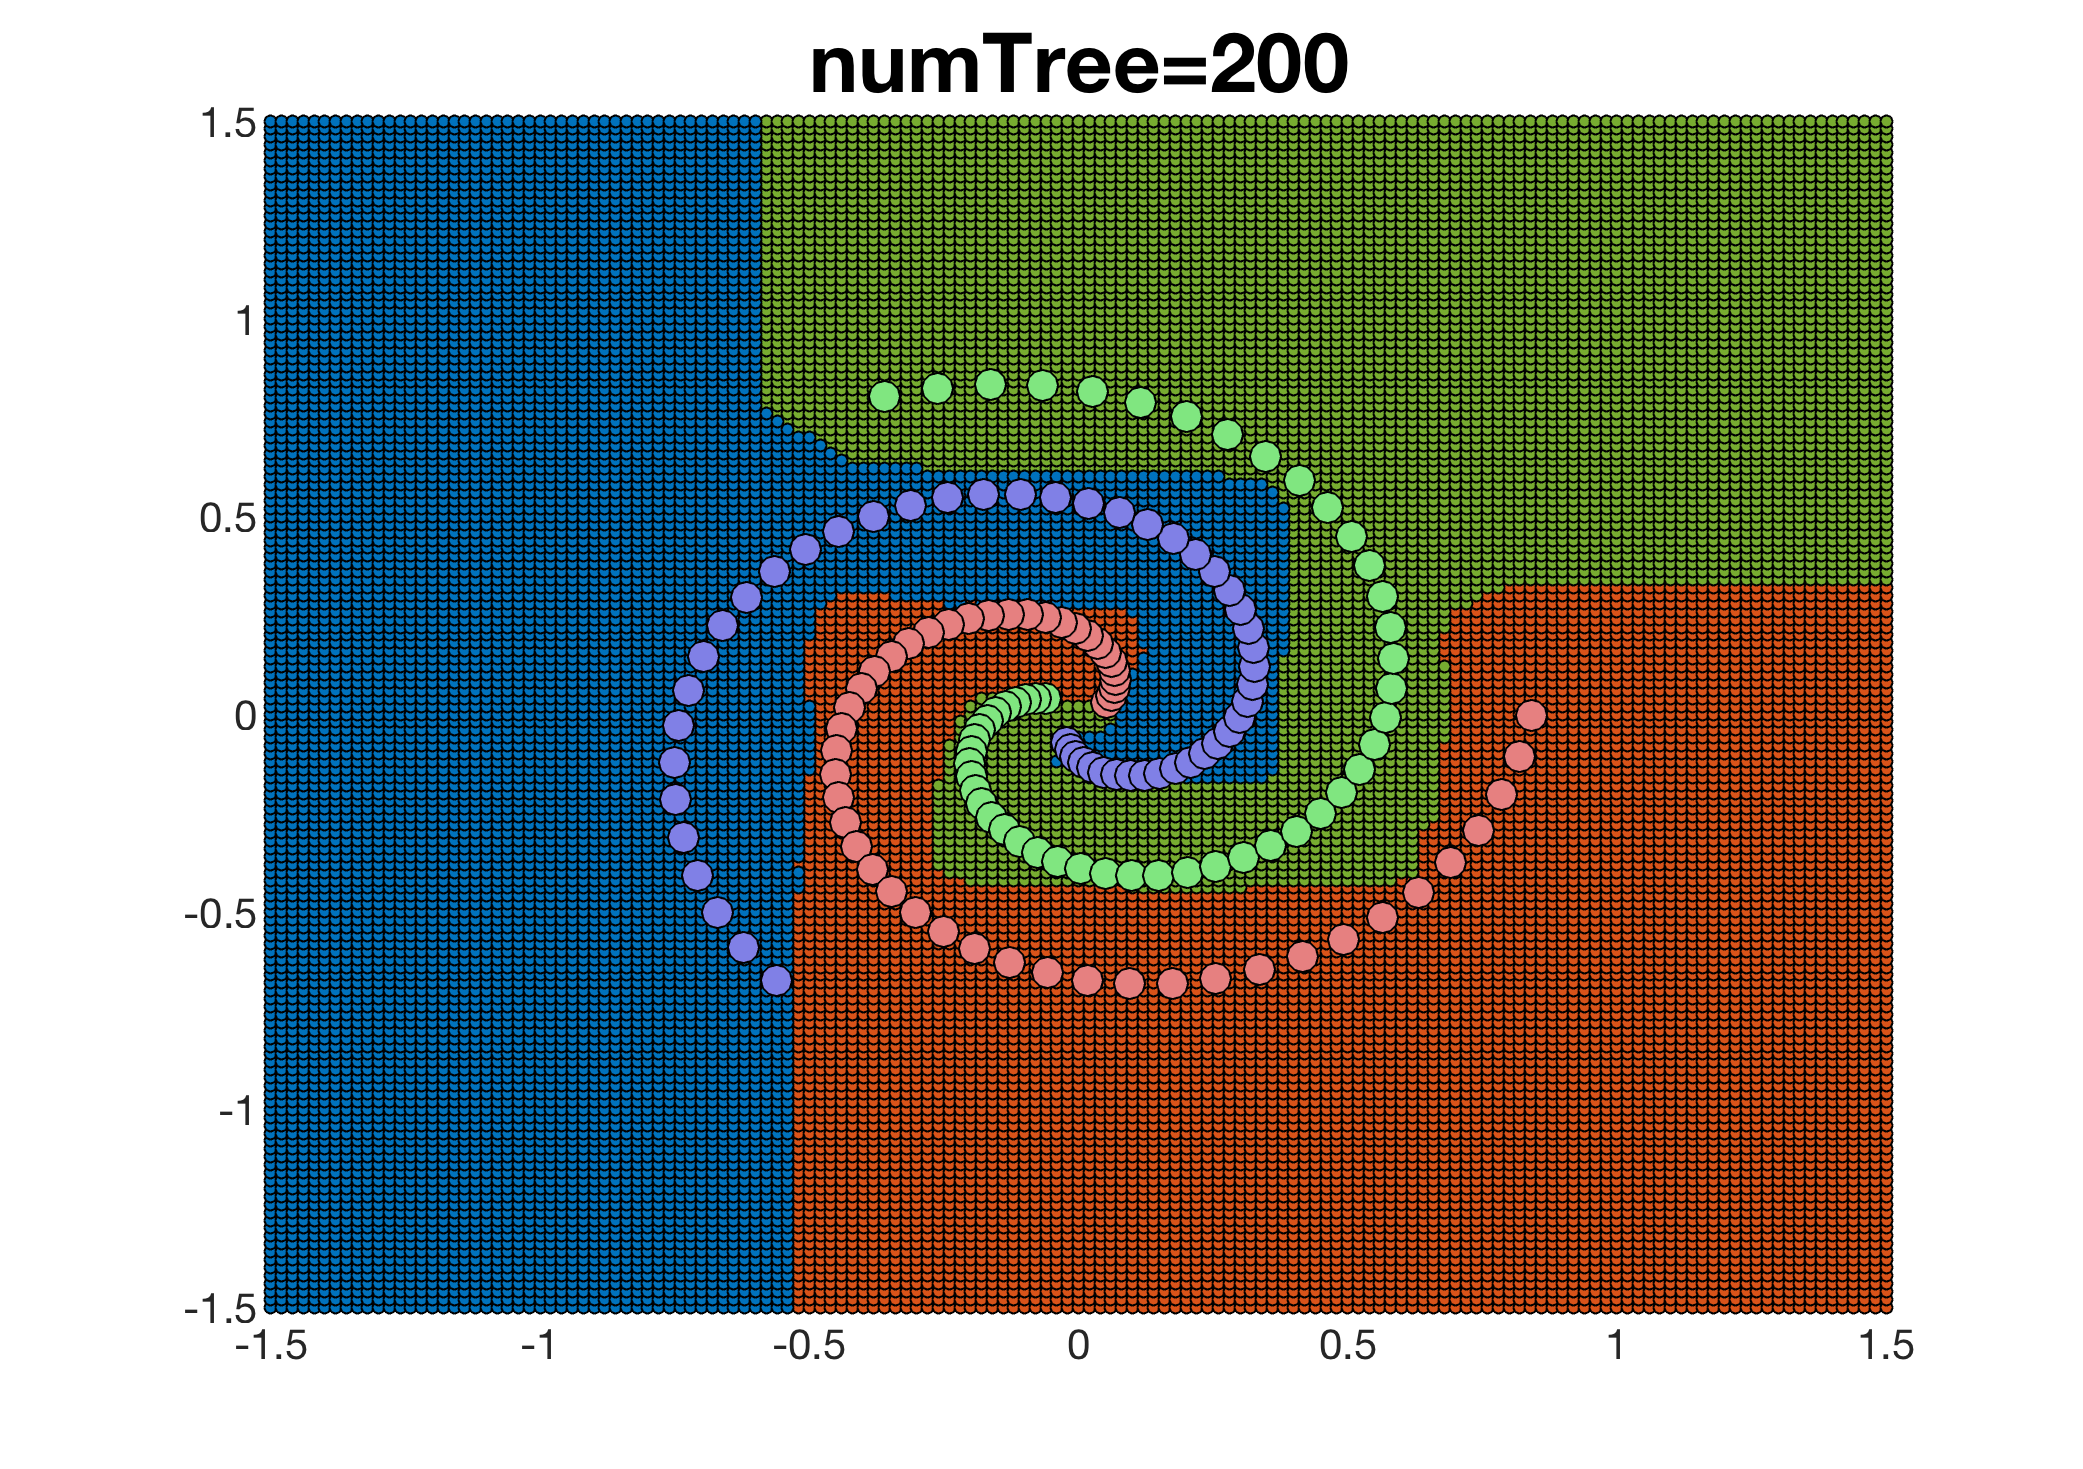
\includegraphics[width=0.40\columnwidth]{ax_200_trees}
    \caption{Overview of spectral subtraction process}
\end{figure}

It is important to note that increasing the number of trees has computation costs associated with it. Although this was not evident when dealing with the toy spiral dataset, the computational penalty that one has to pay for increasing the number of trees becomes abundantly clear when dealing with the Caltech 101 datset. 

\subsection{Varying Number of Split Functions}

Next, we vary the number of split functions, \texttt{param.numTree} is fixed at $10$. By increasing the number of split functions that we try, we are decreasing the randomness of inherent within each tree. If all trees are assumed to be completely uncorrelated, then $E_{com}=\nicefrac{E_{av}}{T}$; where $E_{com}$ is the error incurred by the random forest and $E_{av}$ is the average error of each tree. If the trees are correlated, then $E_{com}\leq\nicefrac{E_{av}}{T}$. Note that, even with correlated trees, it is possible that the committee machine produces good results with $E_{av}$ is low. A good balance point has to be found, such that to achieve a low $E_{av}$, some correlation is allowed. Observe below that with small number of split numbers, artifacts are observed. Each tree is a very bad learner and thus, even though $E_{com}\approx\nicefrac{E_{av}}{T}$, $E_{com}$ is still rather high. Increasing the number of split functions to $7$, the random forest is clearly trying its best to map the spiral nature of the training data using axis-aligned weak learners. Setting \texttt{param.splitNum} to 15, not only is each tree highly over-fitted, the committee machine cannot average away the over-fitting artifacts because the trees are highly correlated.

\begin{figure}[H]
	\centering
    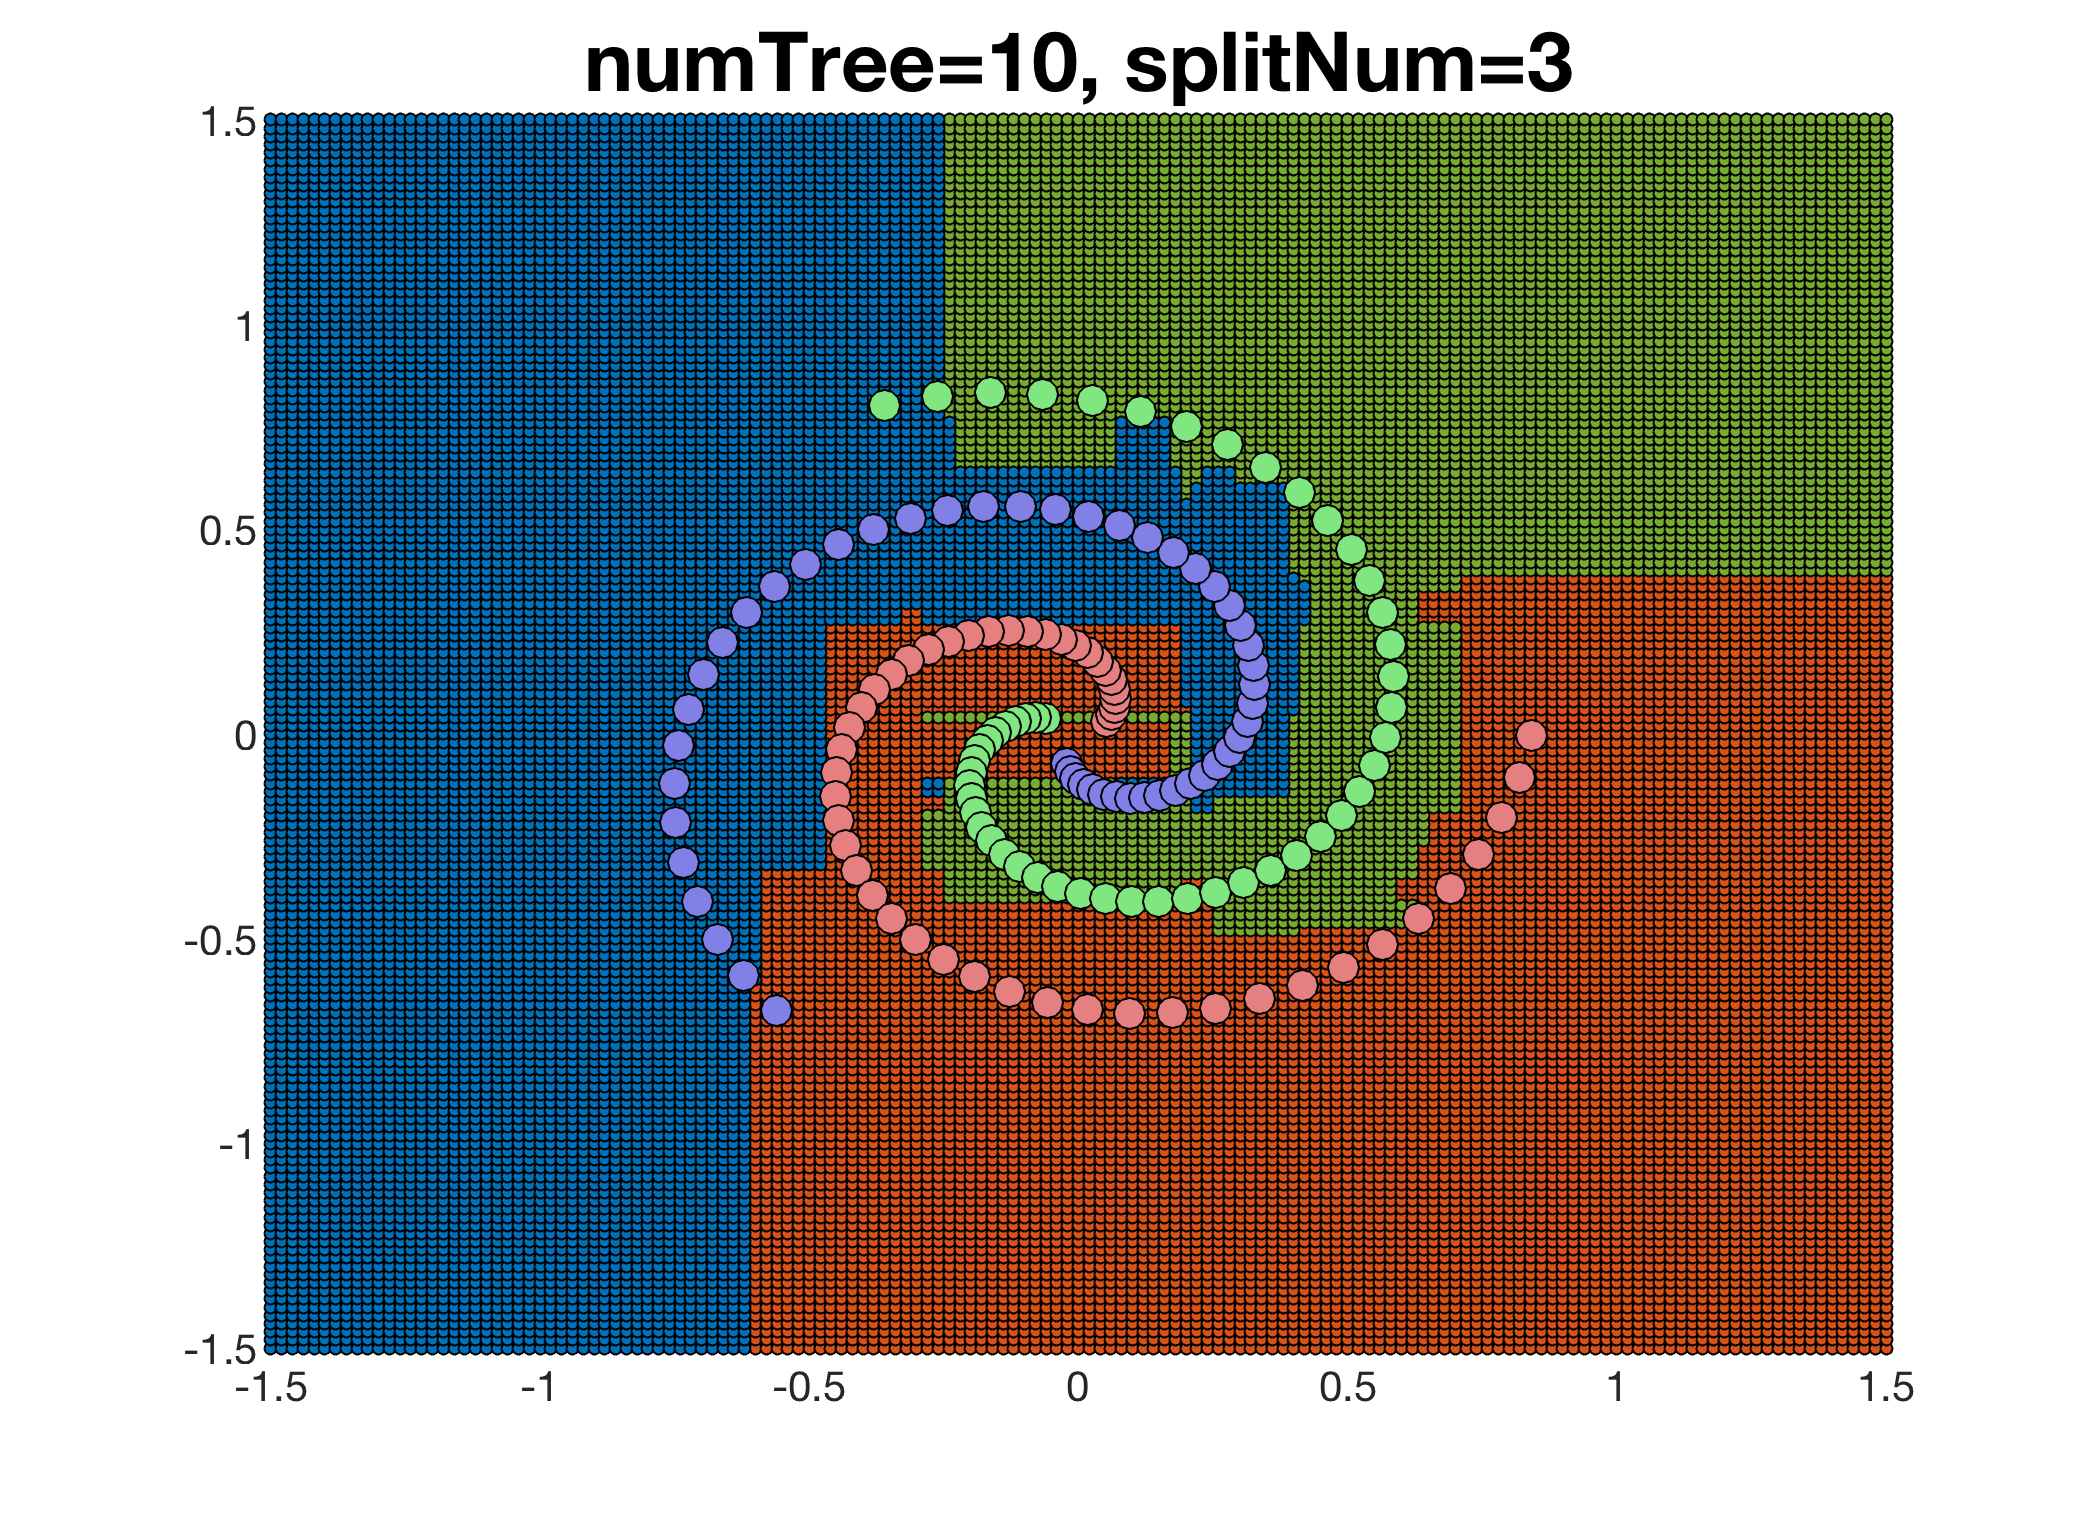
\includegraphics[width=0.40\columnwidth]{splitNum_3}
	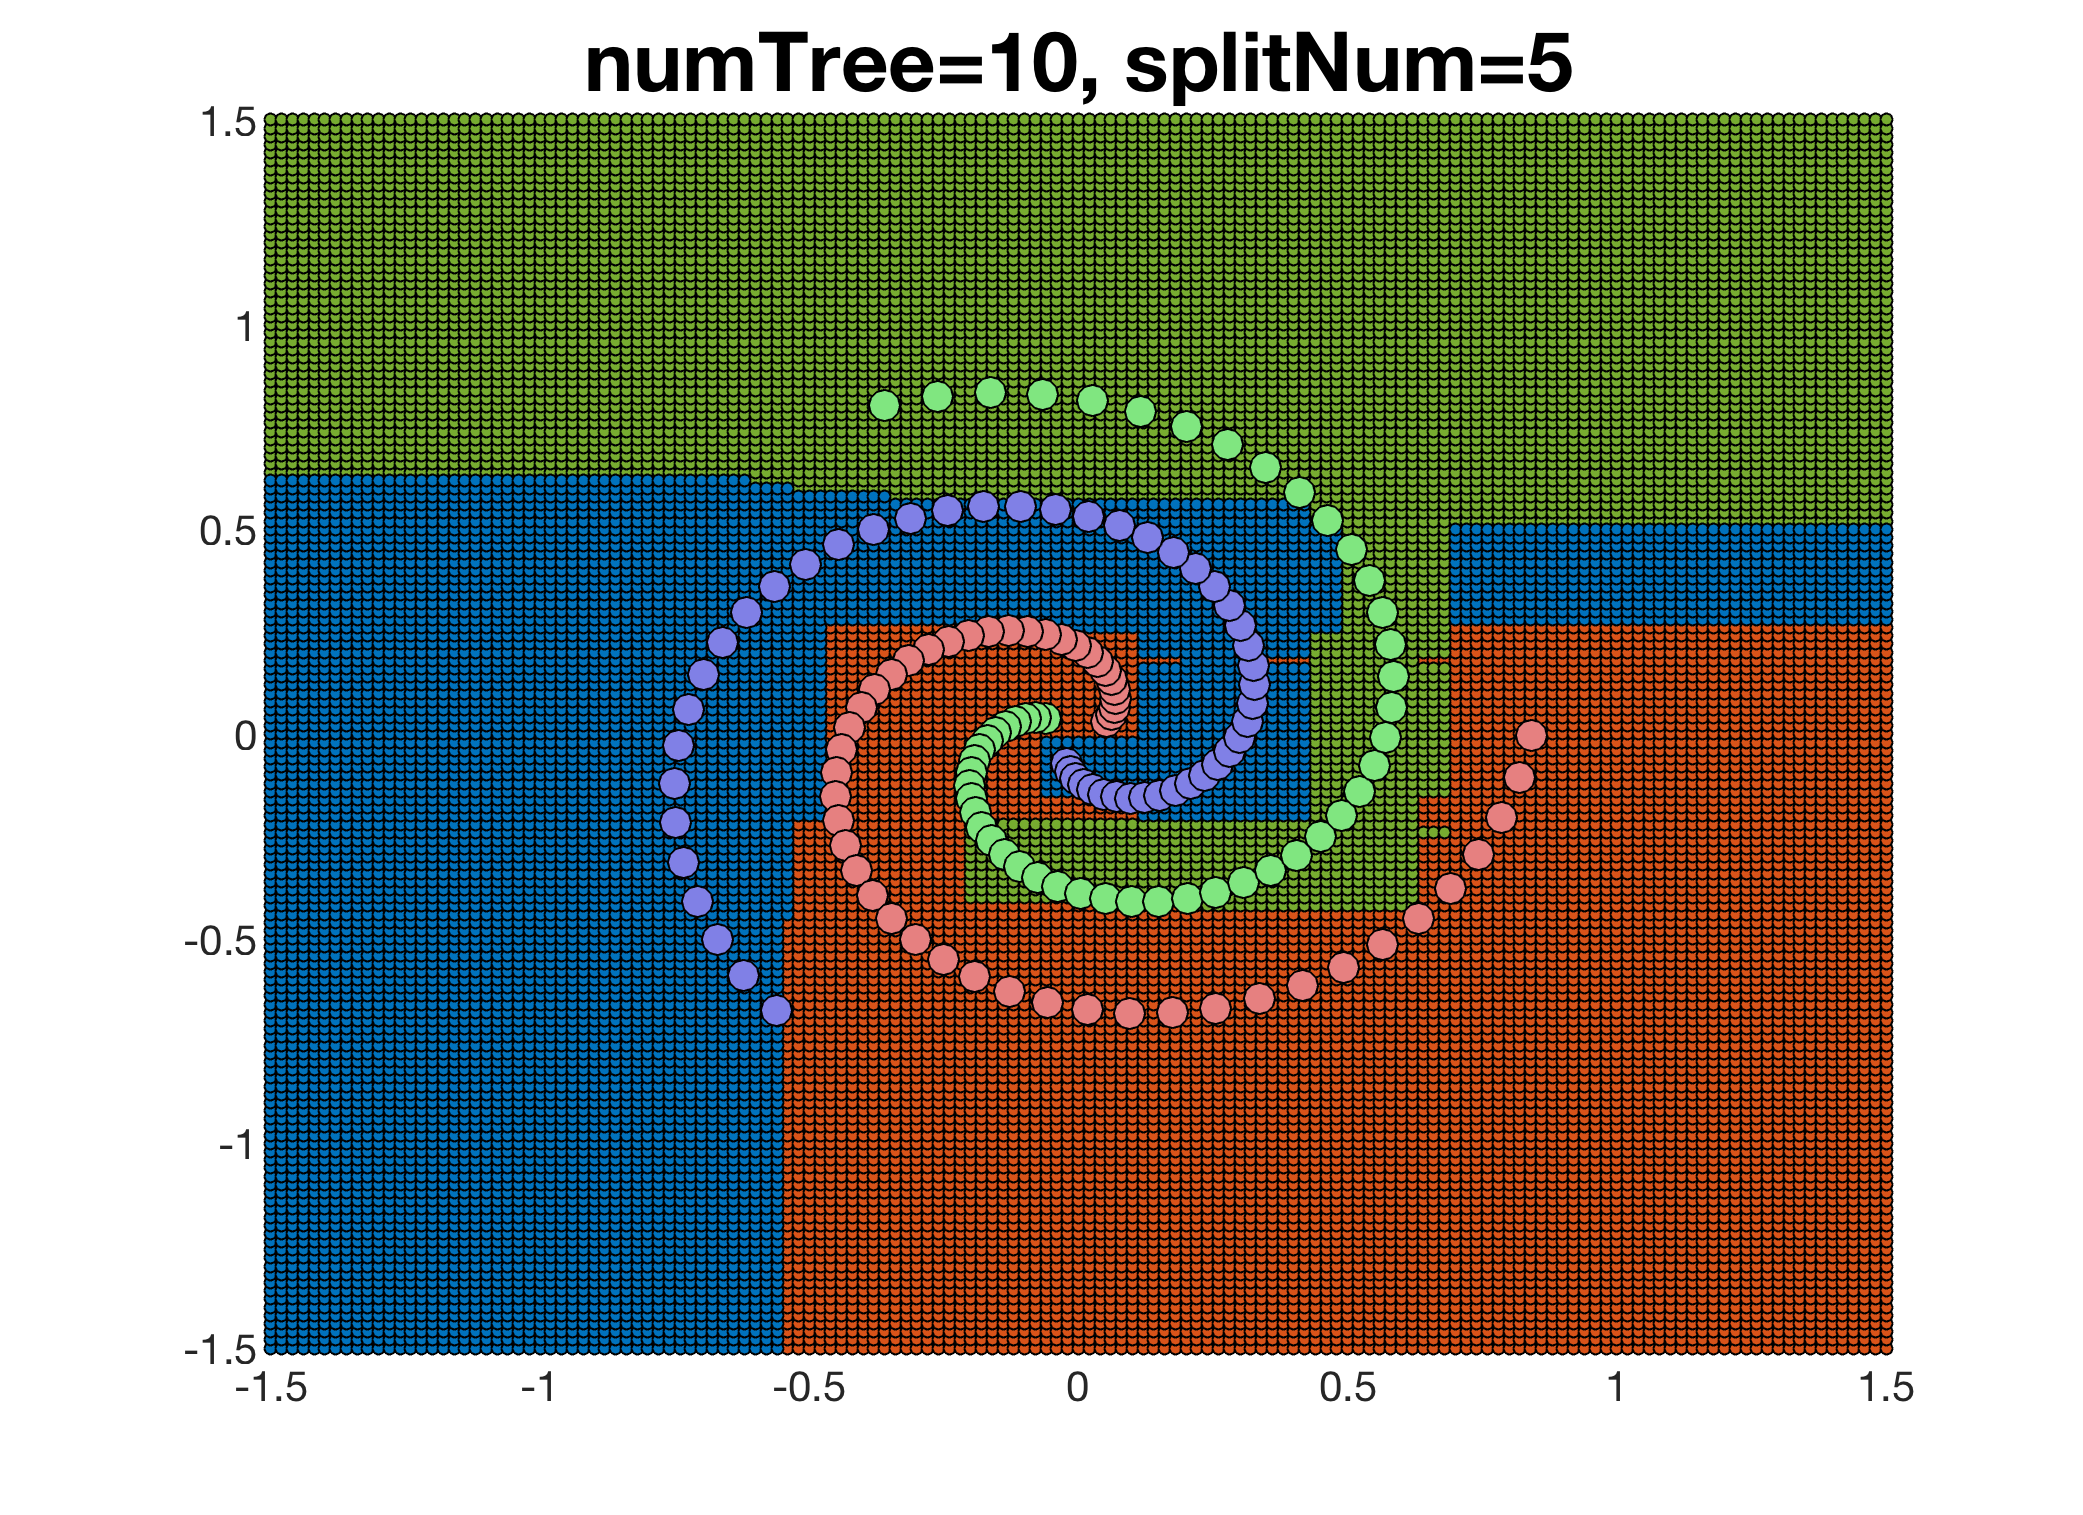
\includegraphics[width=0.40\columnwidth]{splitNum_5}
    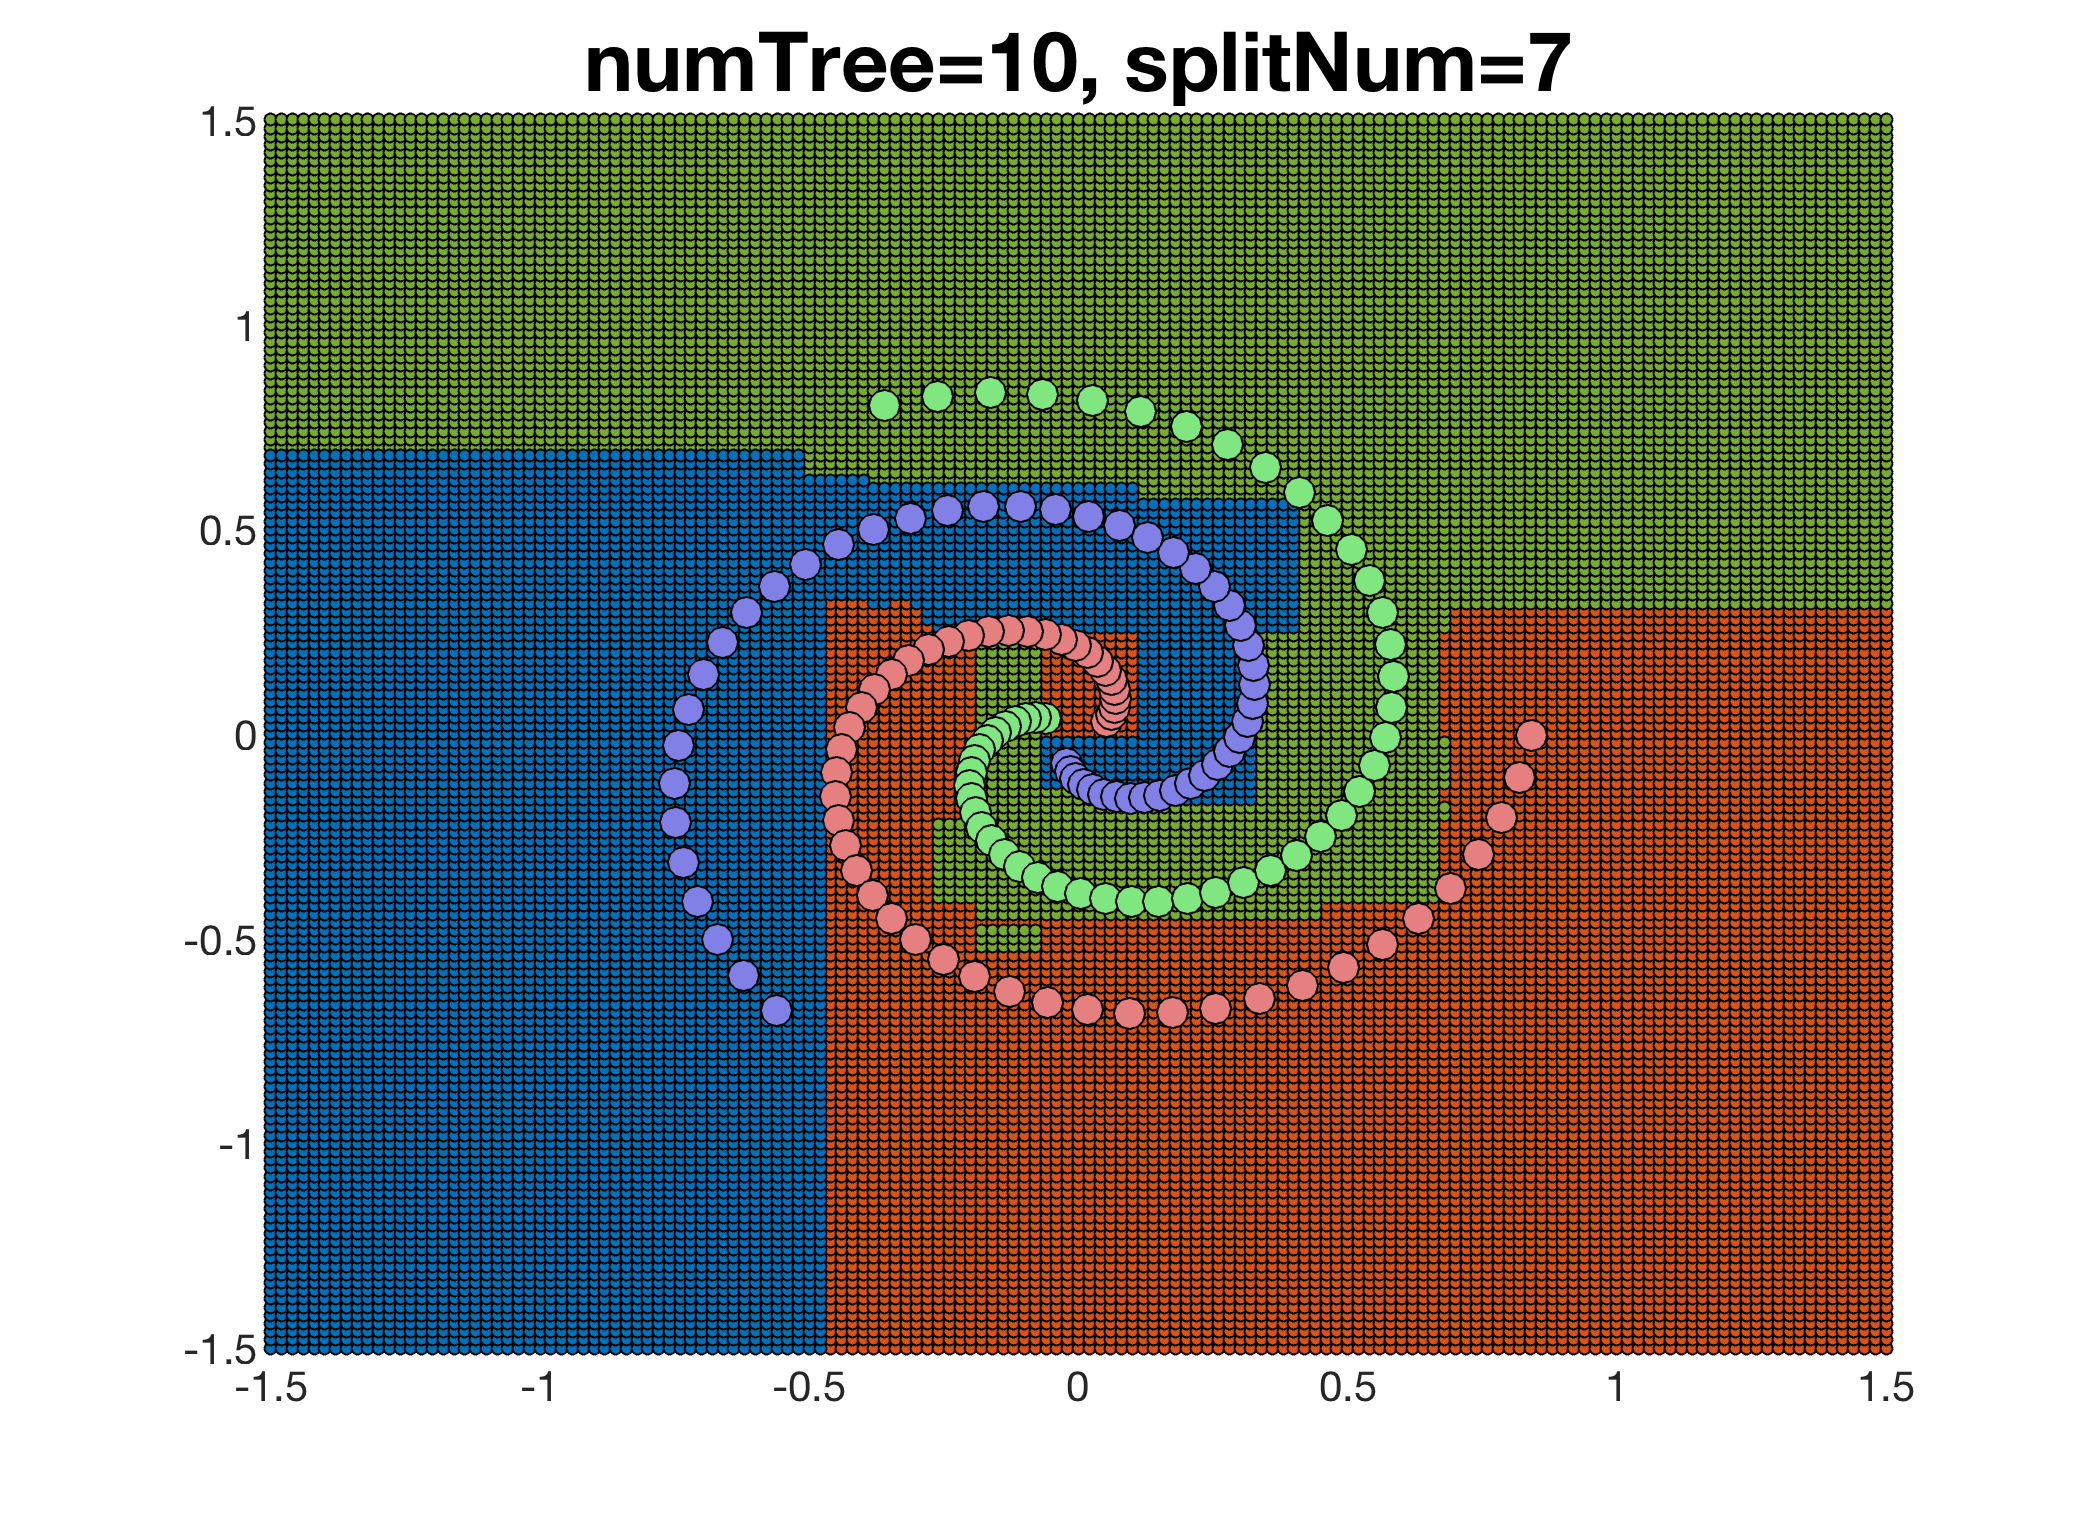
\includegraphics[width=0.40\columnwidth]{splitNum_7}
    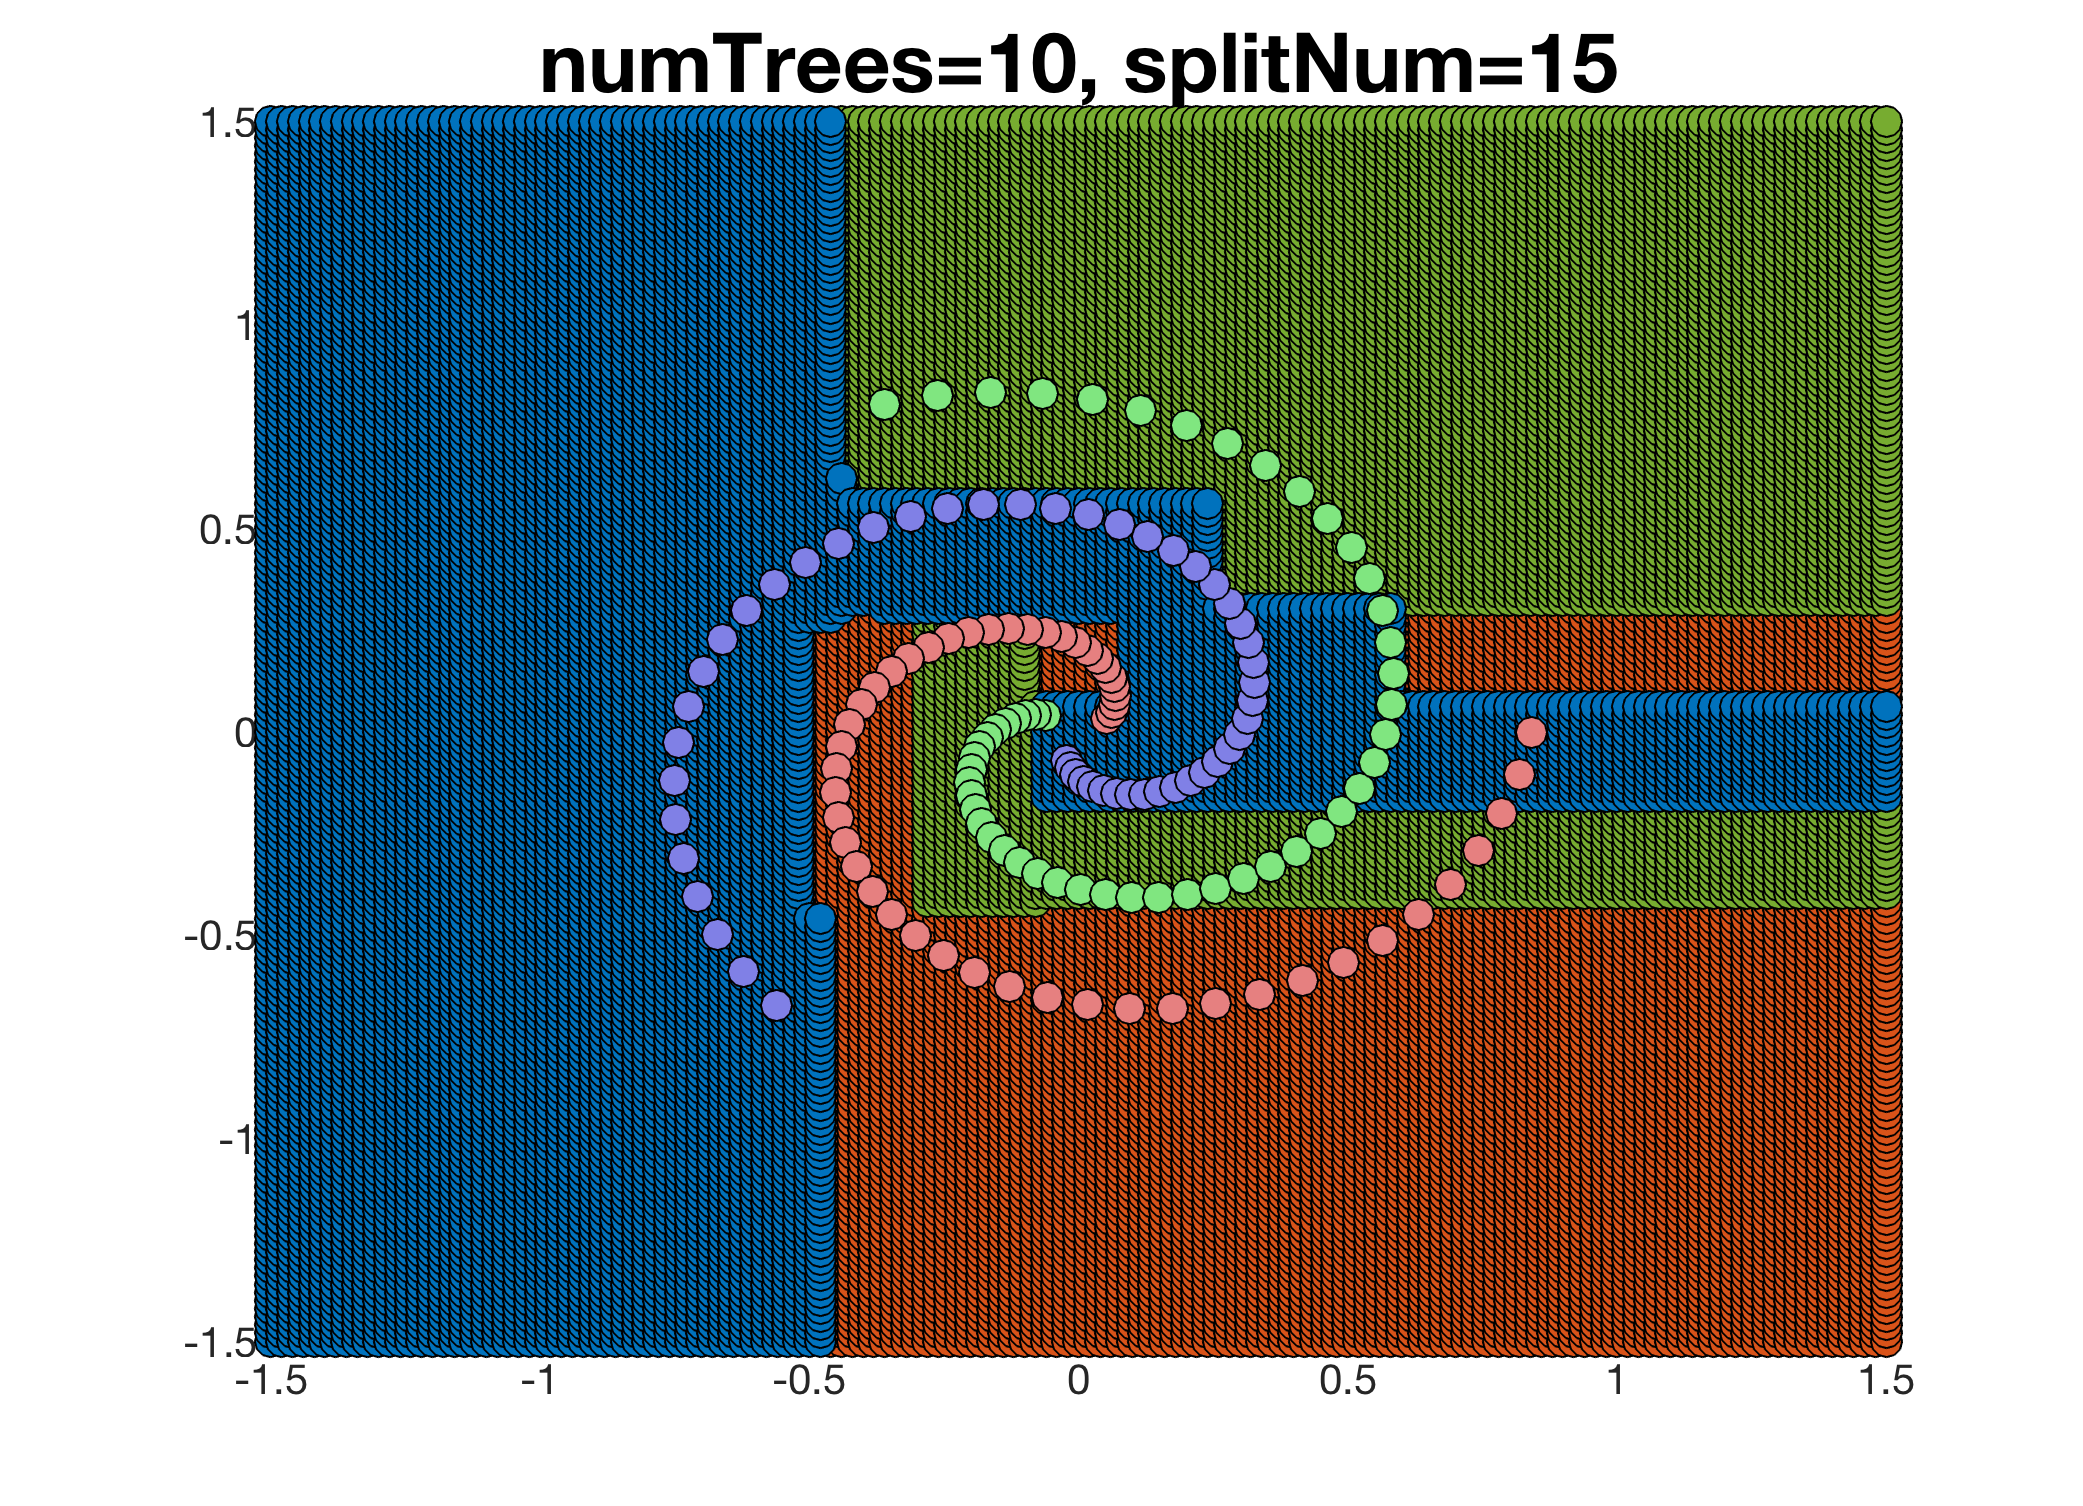
\includegraphics[width=0.40\columnwidth]{splitNum_15}
    \caption{Overview of spectral subtraction process}
\end{figure}

\subsection{Varying Tree Depth}

The third parameter that can be varied is the depth of the tree. It can be seen that more accurate results are produced when tree depth is increased. With tree depth set at 3 or 5, there are very obvious artifacts that appear; a thin red line when depth is set at 3, and a massive blue region when the depth is set at 5. These are clearly anomalies that have come about because the classes have not been sufficiently refined at the leaf nodes. Increasing the depth to 7, the obvious anomalies have now disappeared but small artifacts still remain at the center of the graph. These can be further refined if the tree depth is increased to 9. 

\begin{figure}[H]
	\centering
    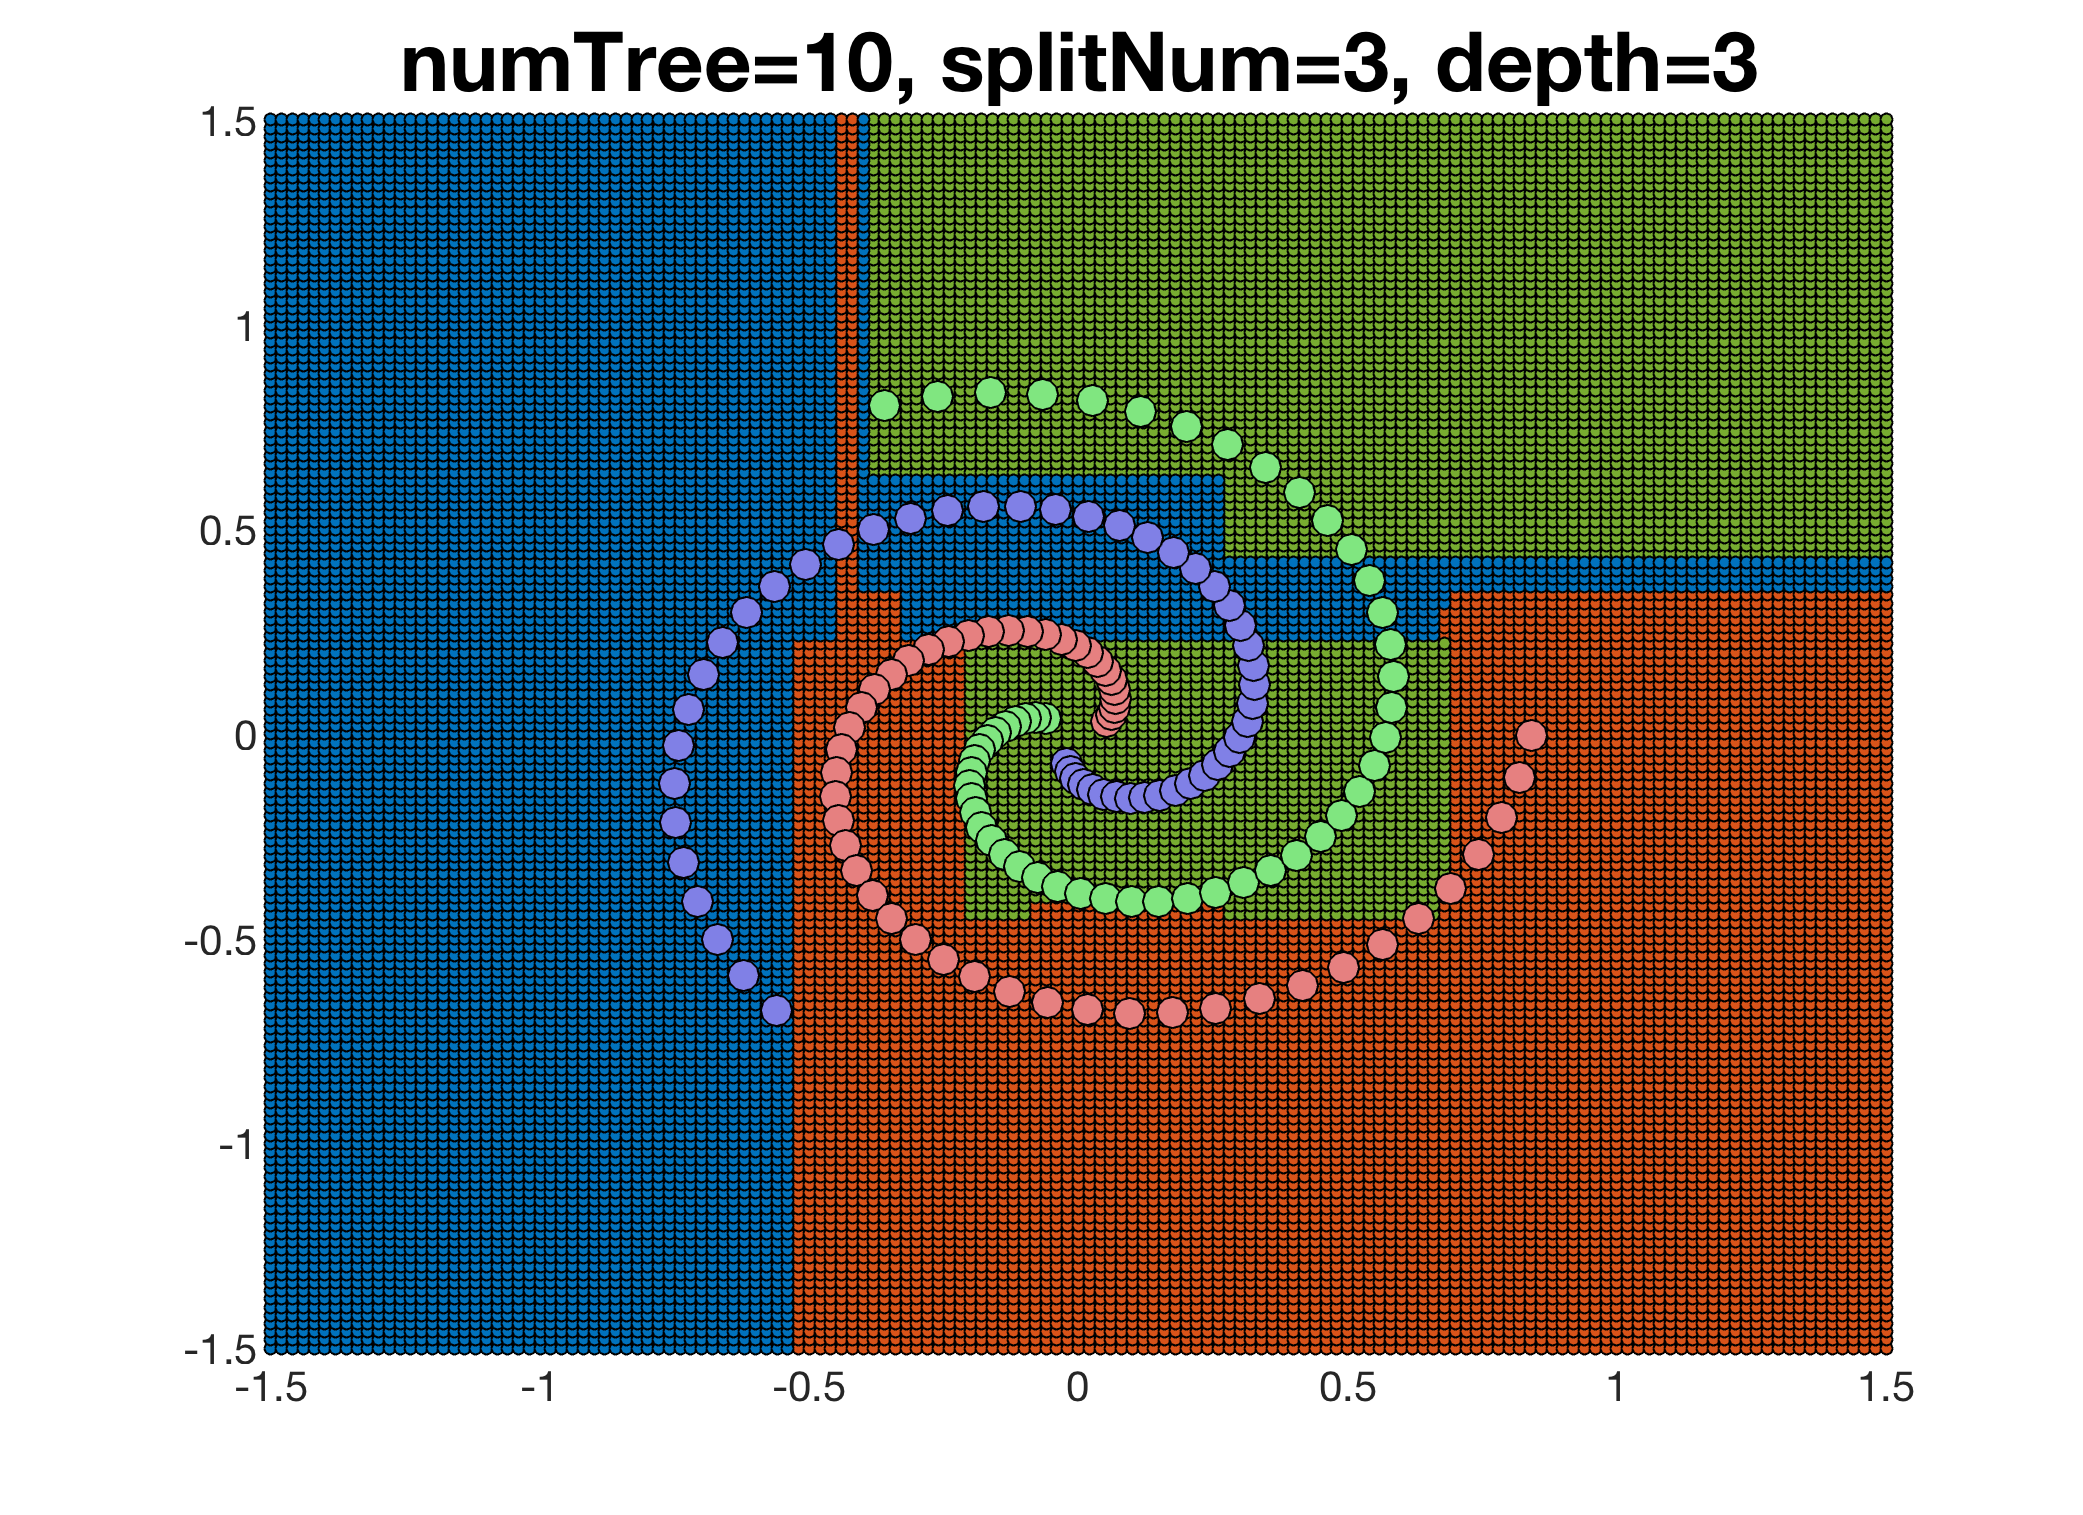
\includegraphics[width=0.40\columnwidth]{tree_depth_3}
	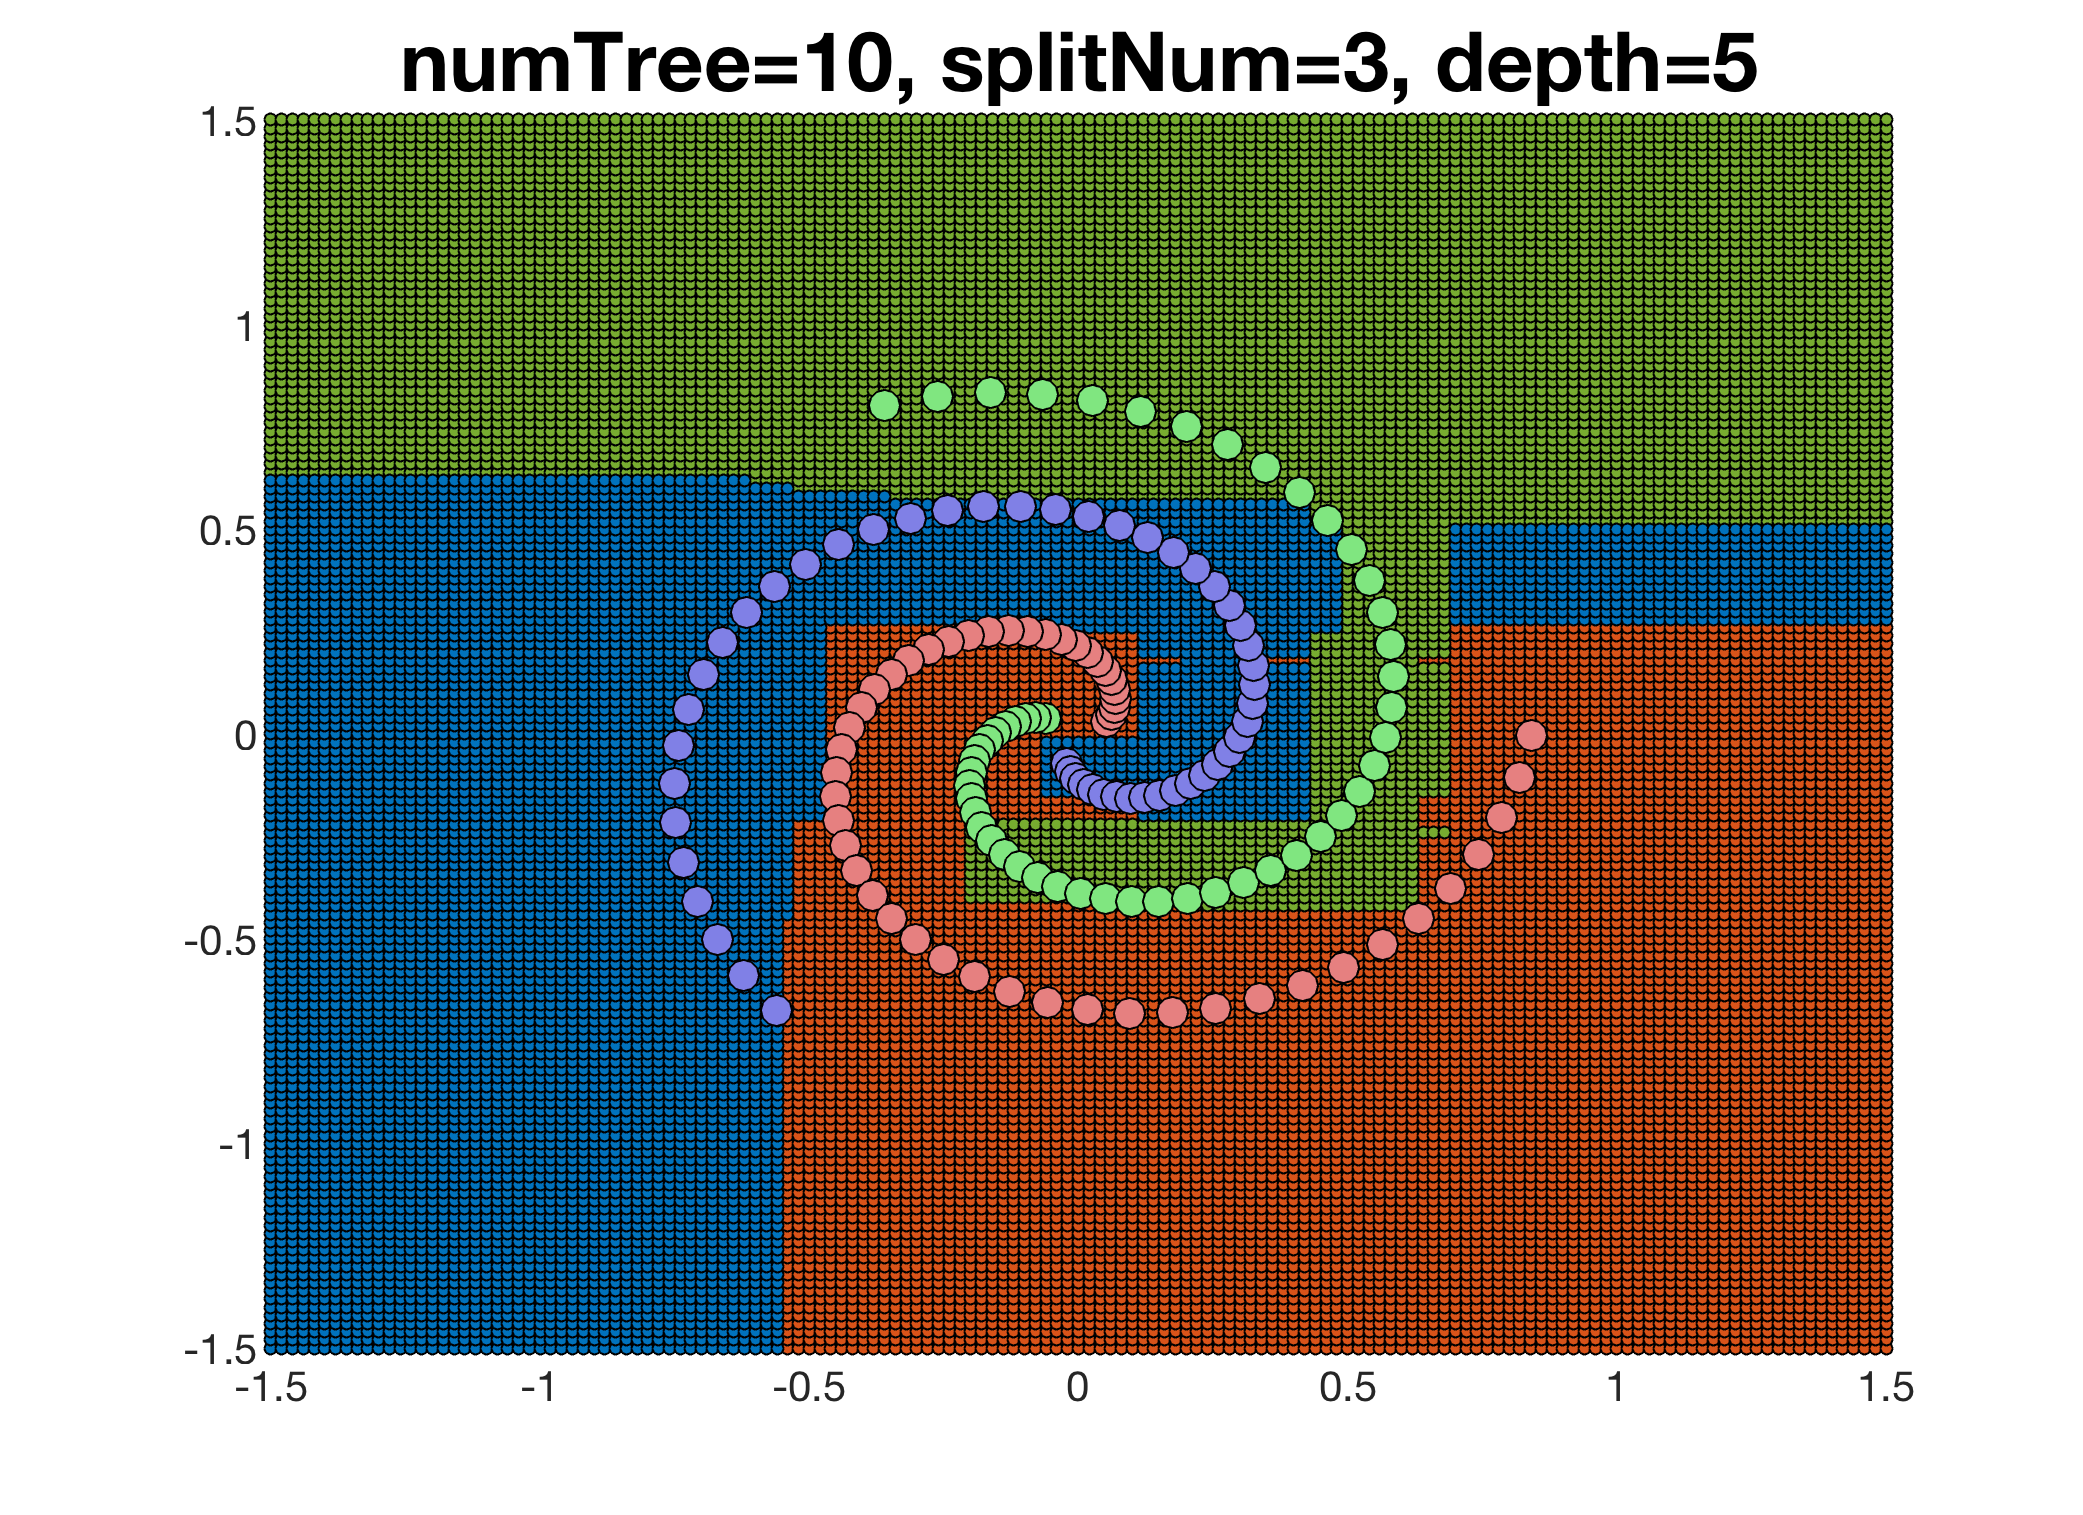
\includegraphics[width=0.40\columnwidth]{tree_depth_5}
    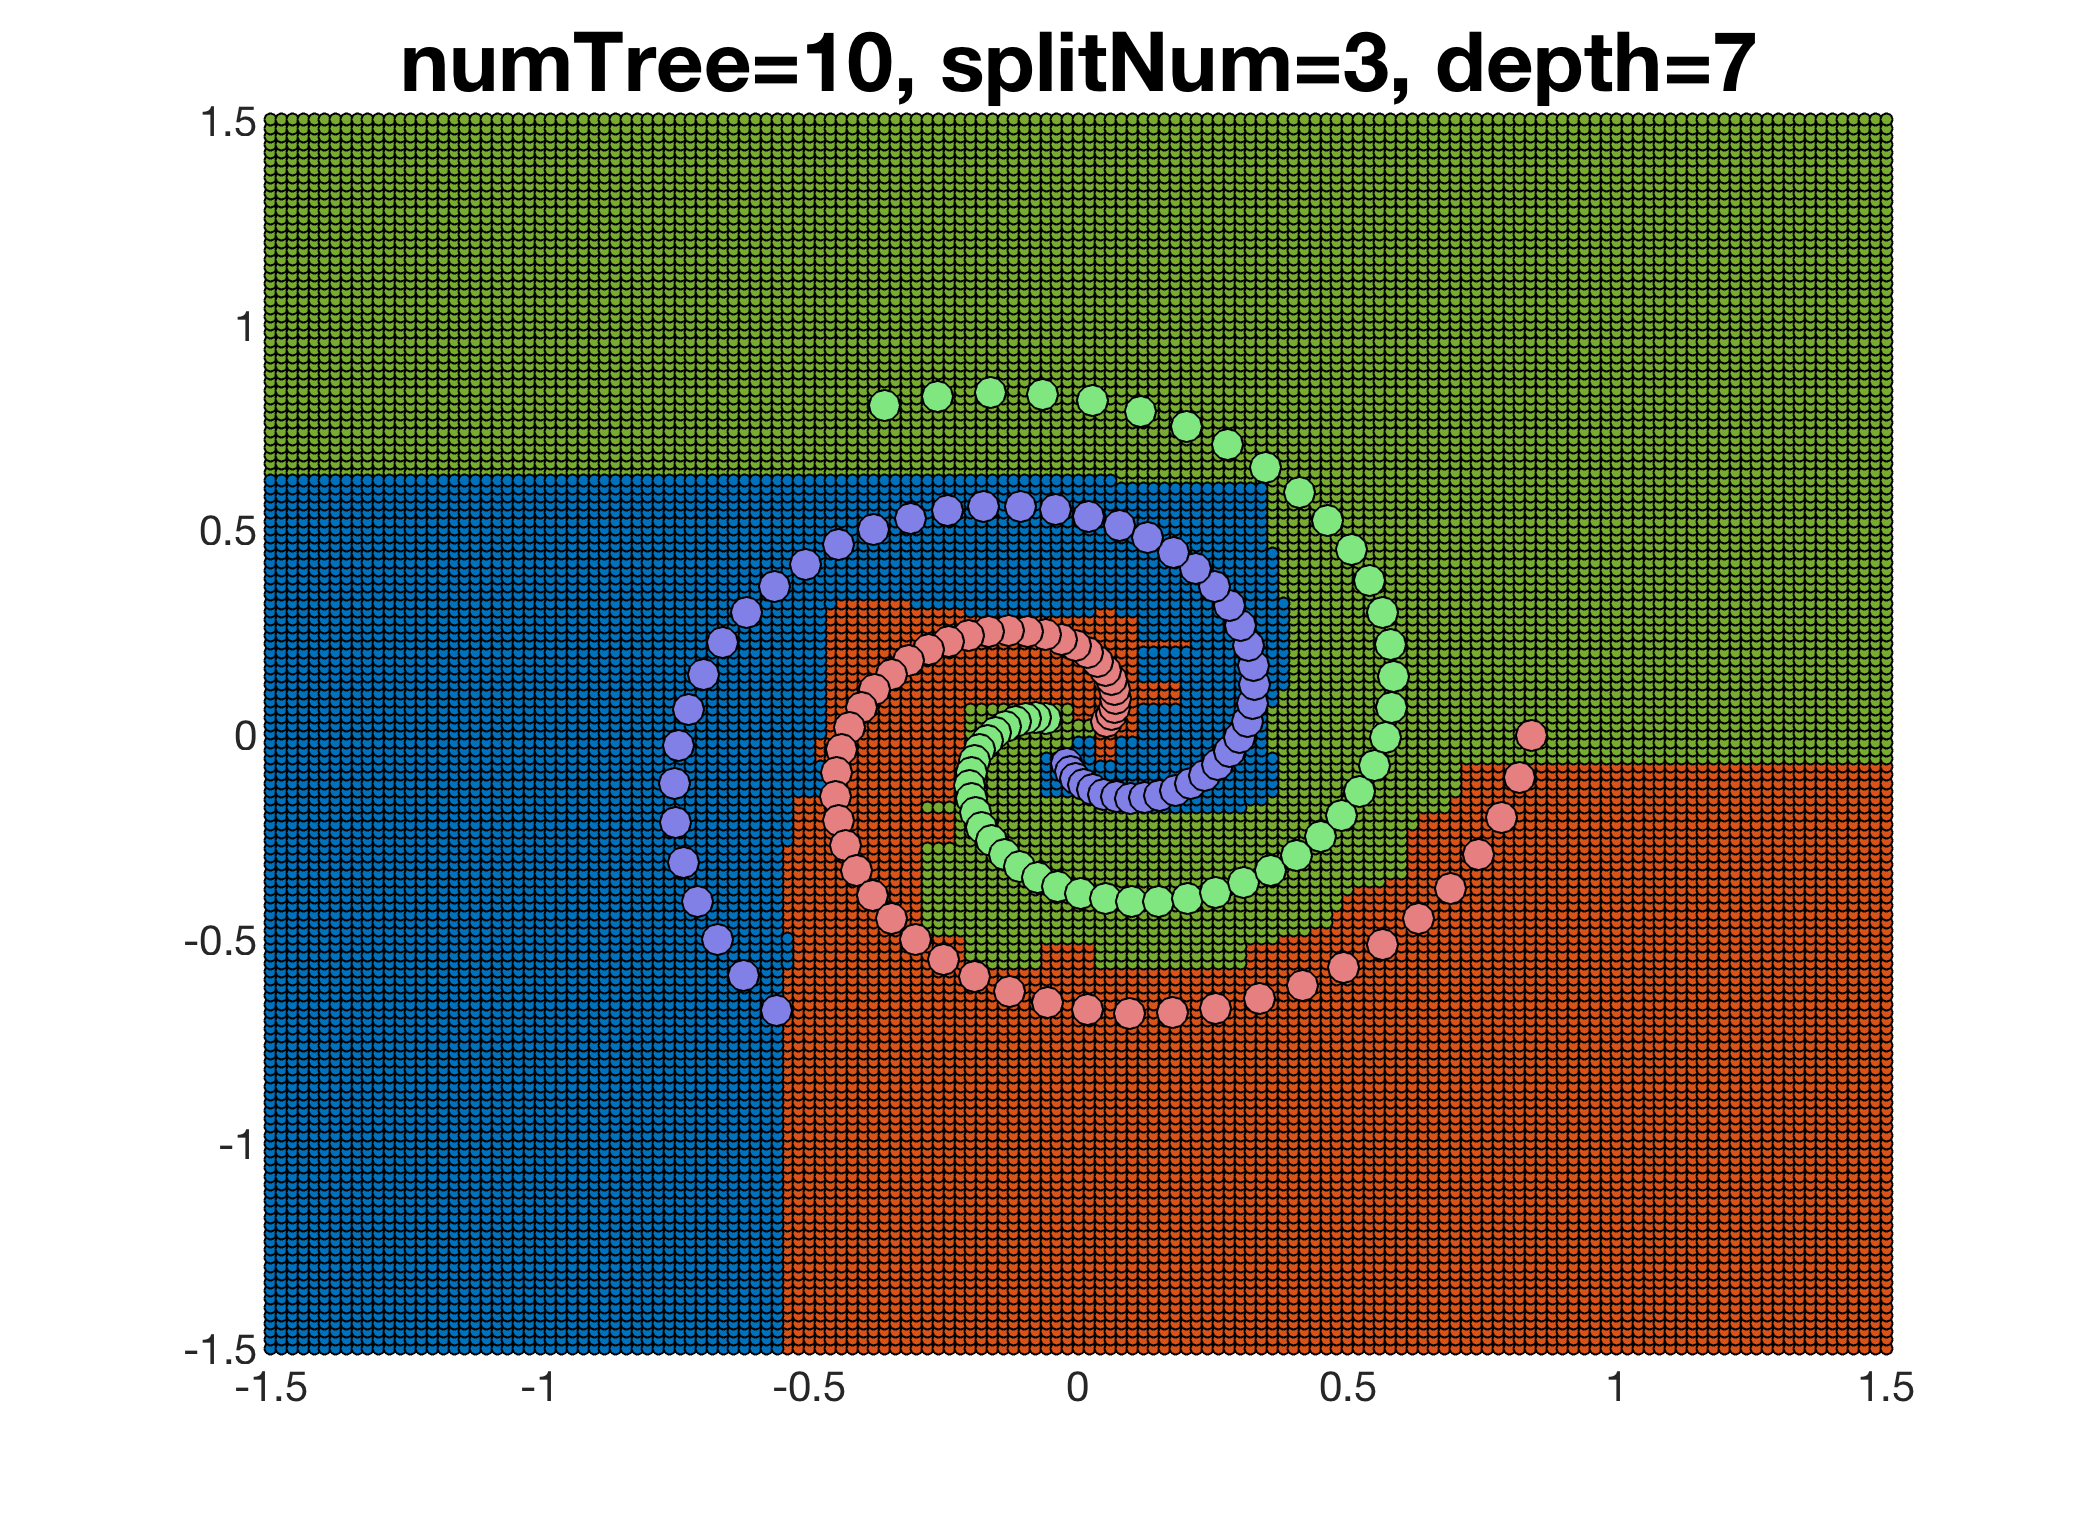
\includegraphics[width=0.40\columnwidth]{tree_depth_7}
    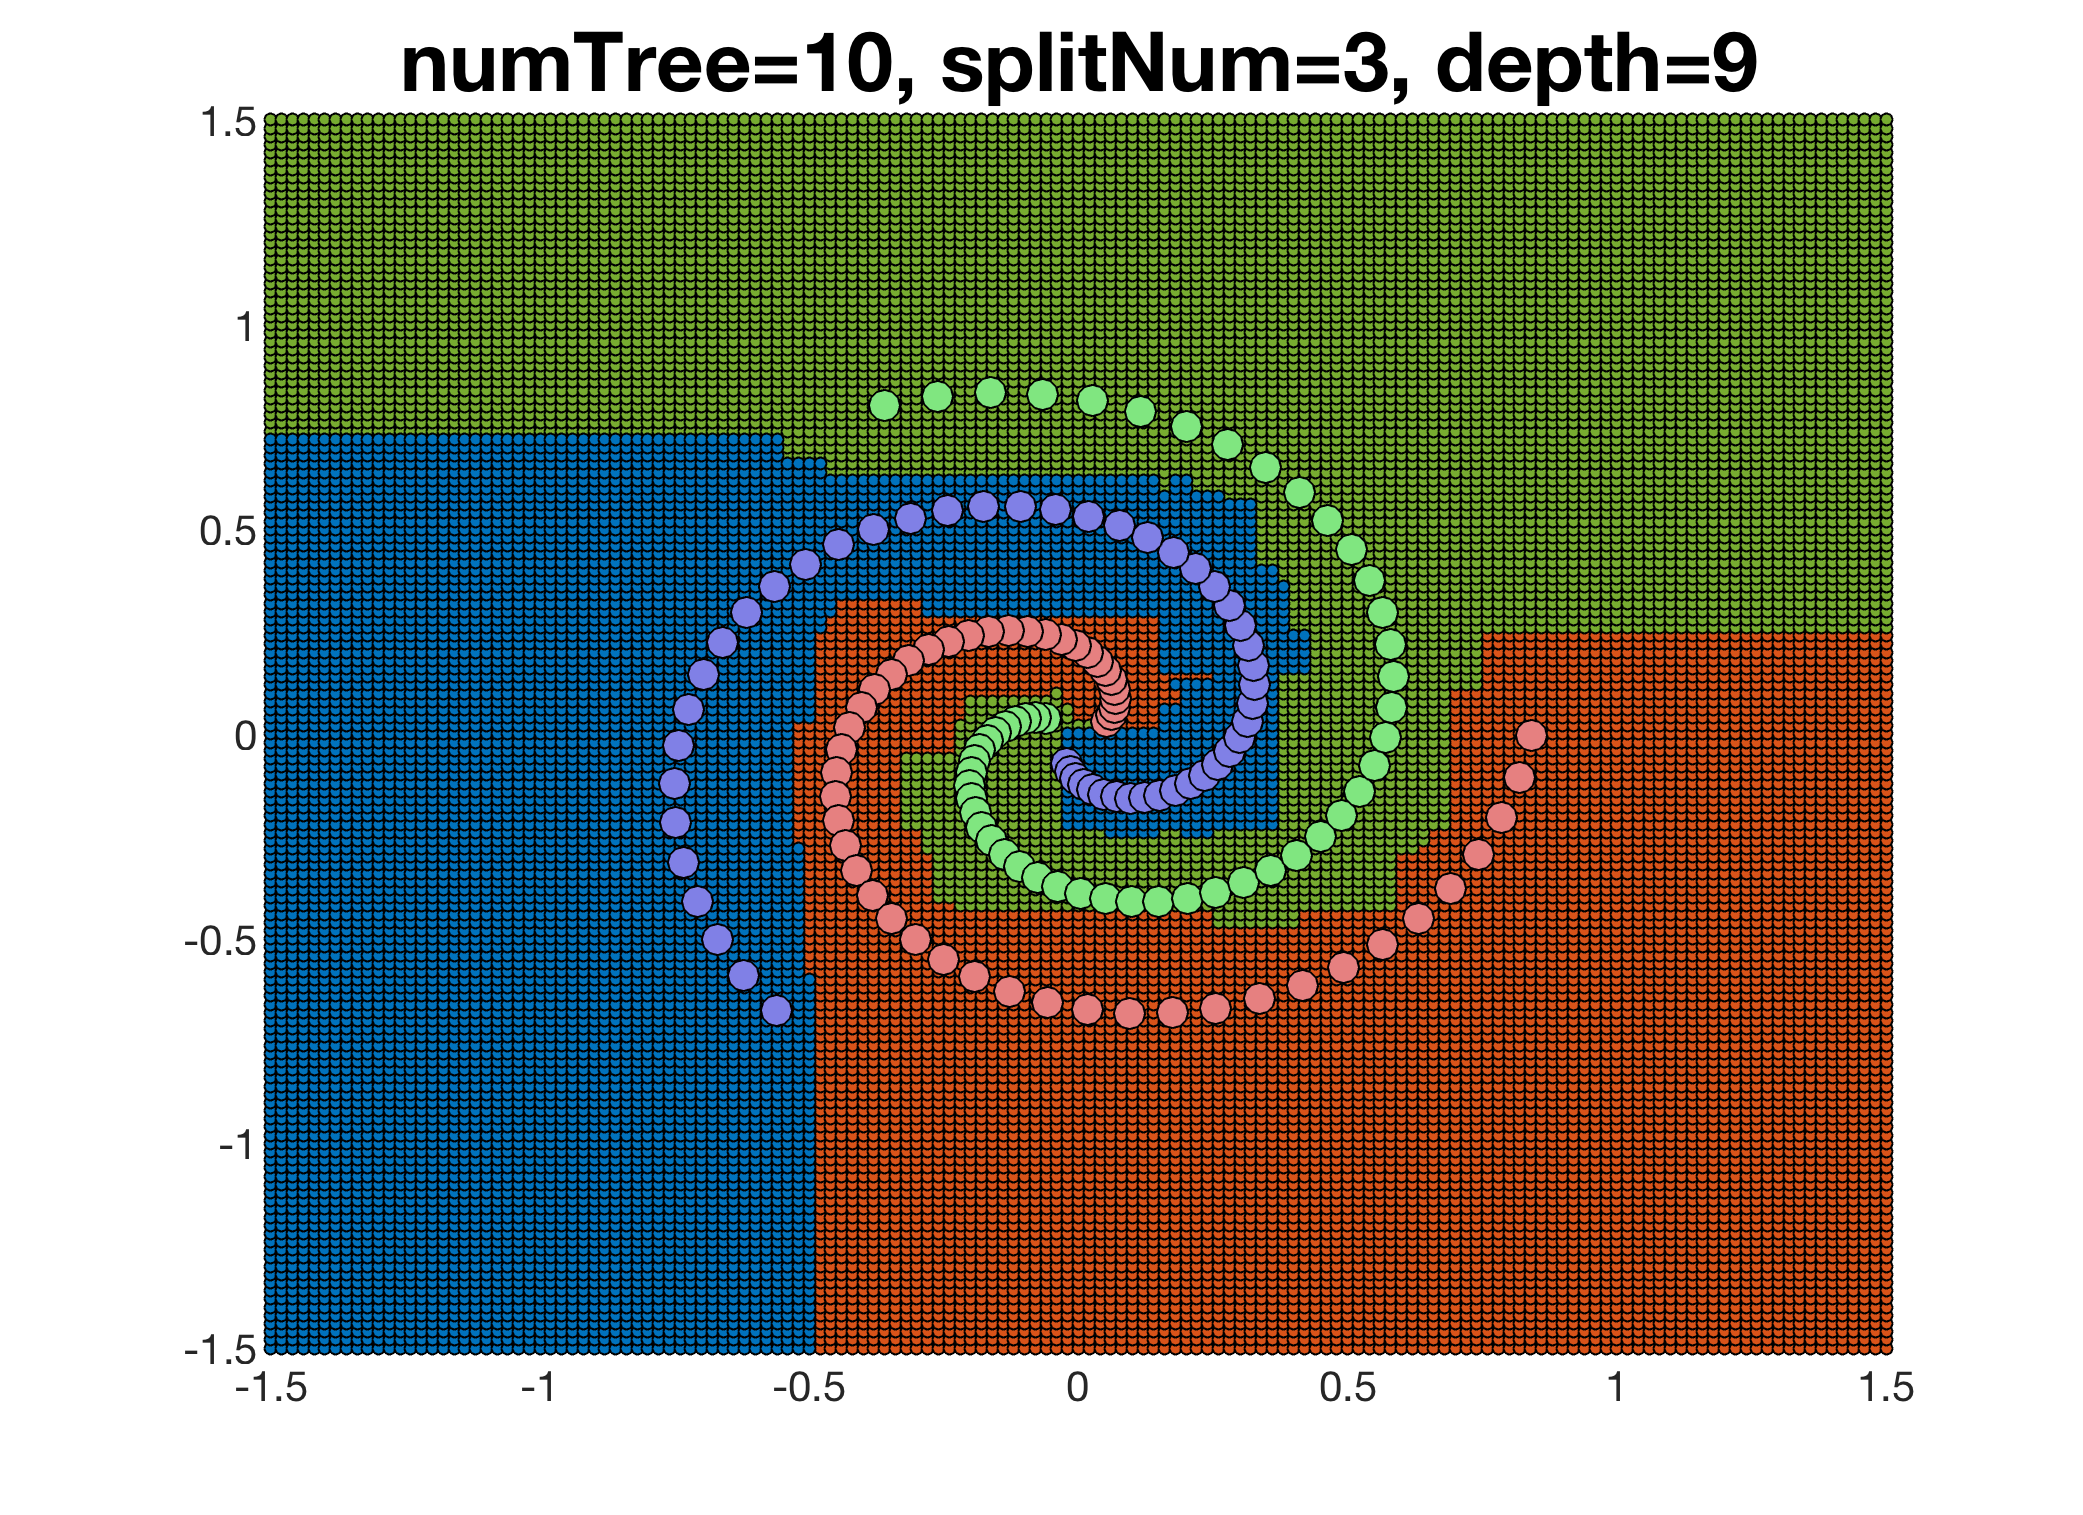
\includegraphics[width=0.40\columnwidth]{tree_depth_9}
    \caption{Overview of spectral subtraction process}
\end{figure}

Tree depth should not be increased arbitrarily for two reasons. As we descend down the tree, training points become refined and get clustered together. If we arbitrarily keep increasing the depth, we will be attempting to separate points which lie very close to one another. The weak-learner will have an effect over the entire range of values for which the algorithm is used. Observe what happens when we train on very few number of points in Figure \ref{fig:learners_2} .

Secondly, increasing tree depth will increase computational complexity exponentially. It is much wiser to average out anomalies using a greater number of trees because while trees can be trained and tested in parallel, each tree must be grown sequentially.


\subsection{Testing with Different Weak Learners}

Note that all the discussion above has all been made with respect to the axis-aligned weak learner. This is important to note that ideal values of splitNum and the tree depth vary with the weak learner used. The graphs below show the effects of using different weak-learner classes. Notice that the class boundaries in the extrapolated region follow the general shape of the learner class used. For reference, an random forest trained using the axis-aligned weak learner with all 3 parameters turned has also been graphed.

\begin{figure}[H]
	\centering
    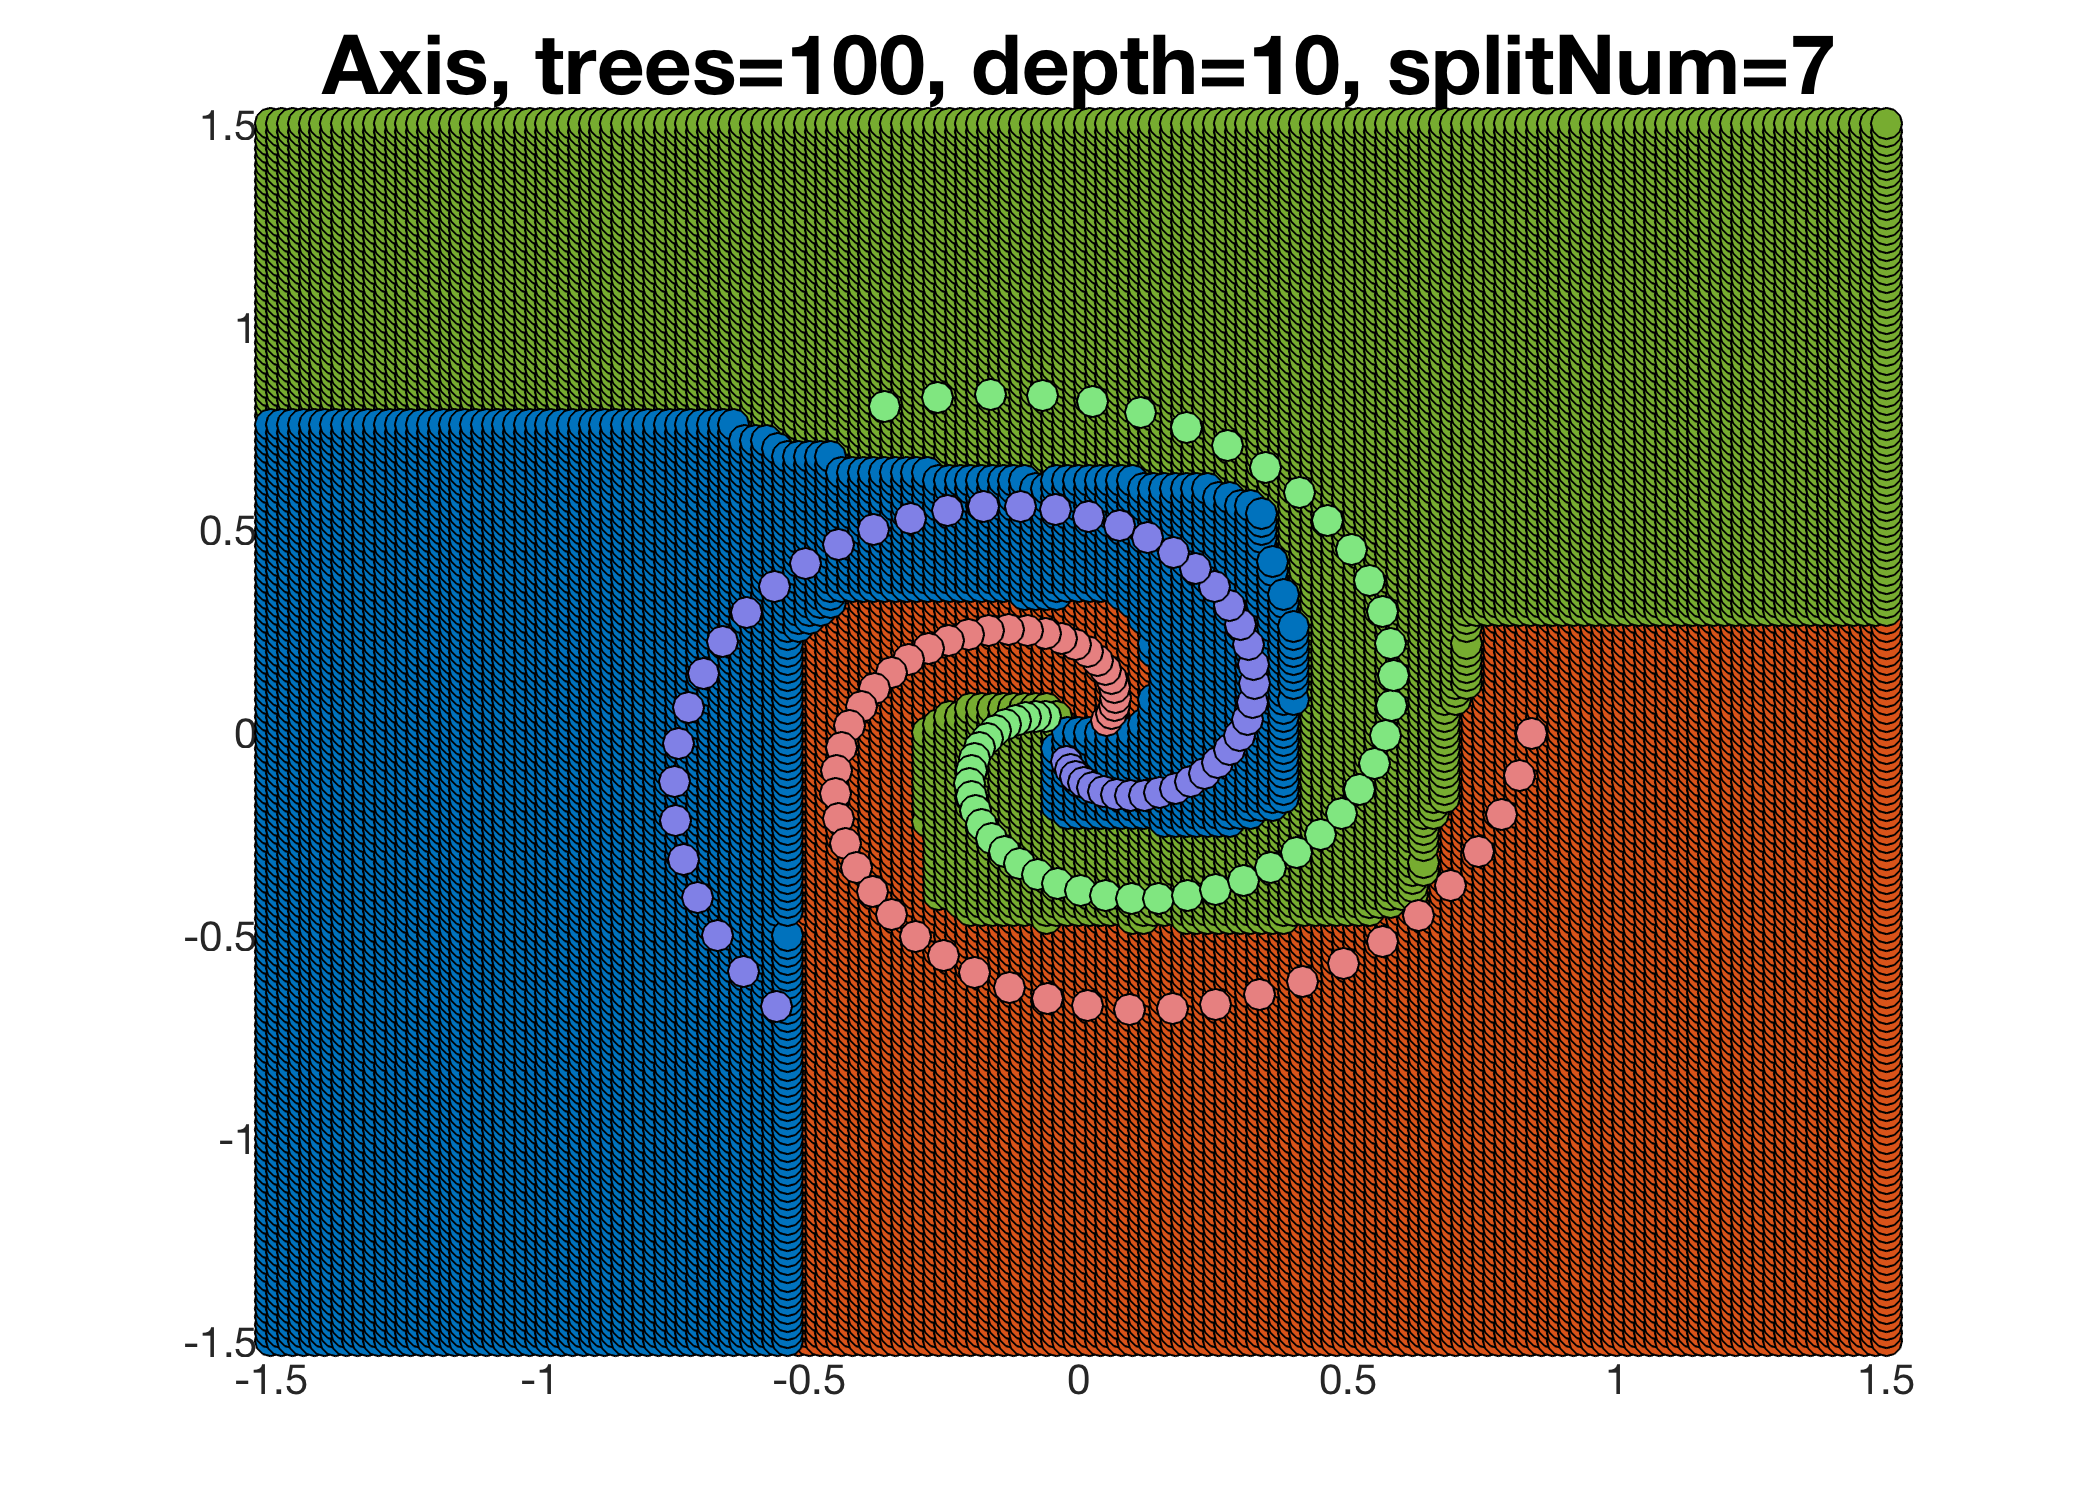
\includegraphics[width=0.40\columnwidth]{axis}
	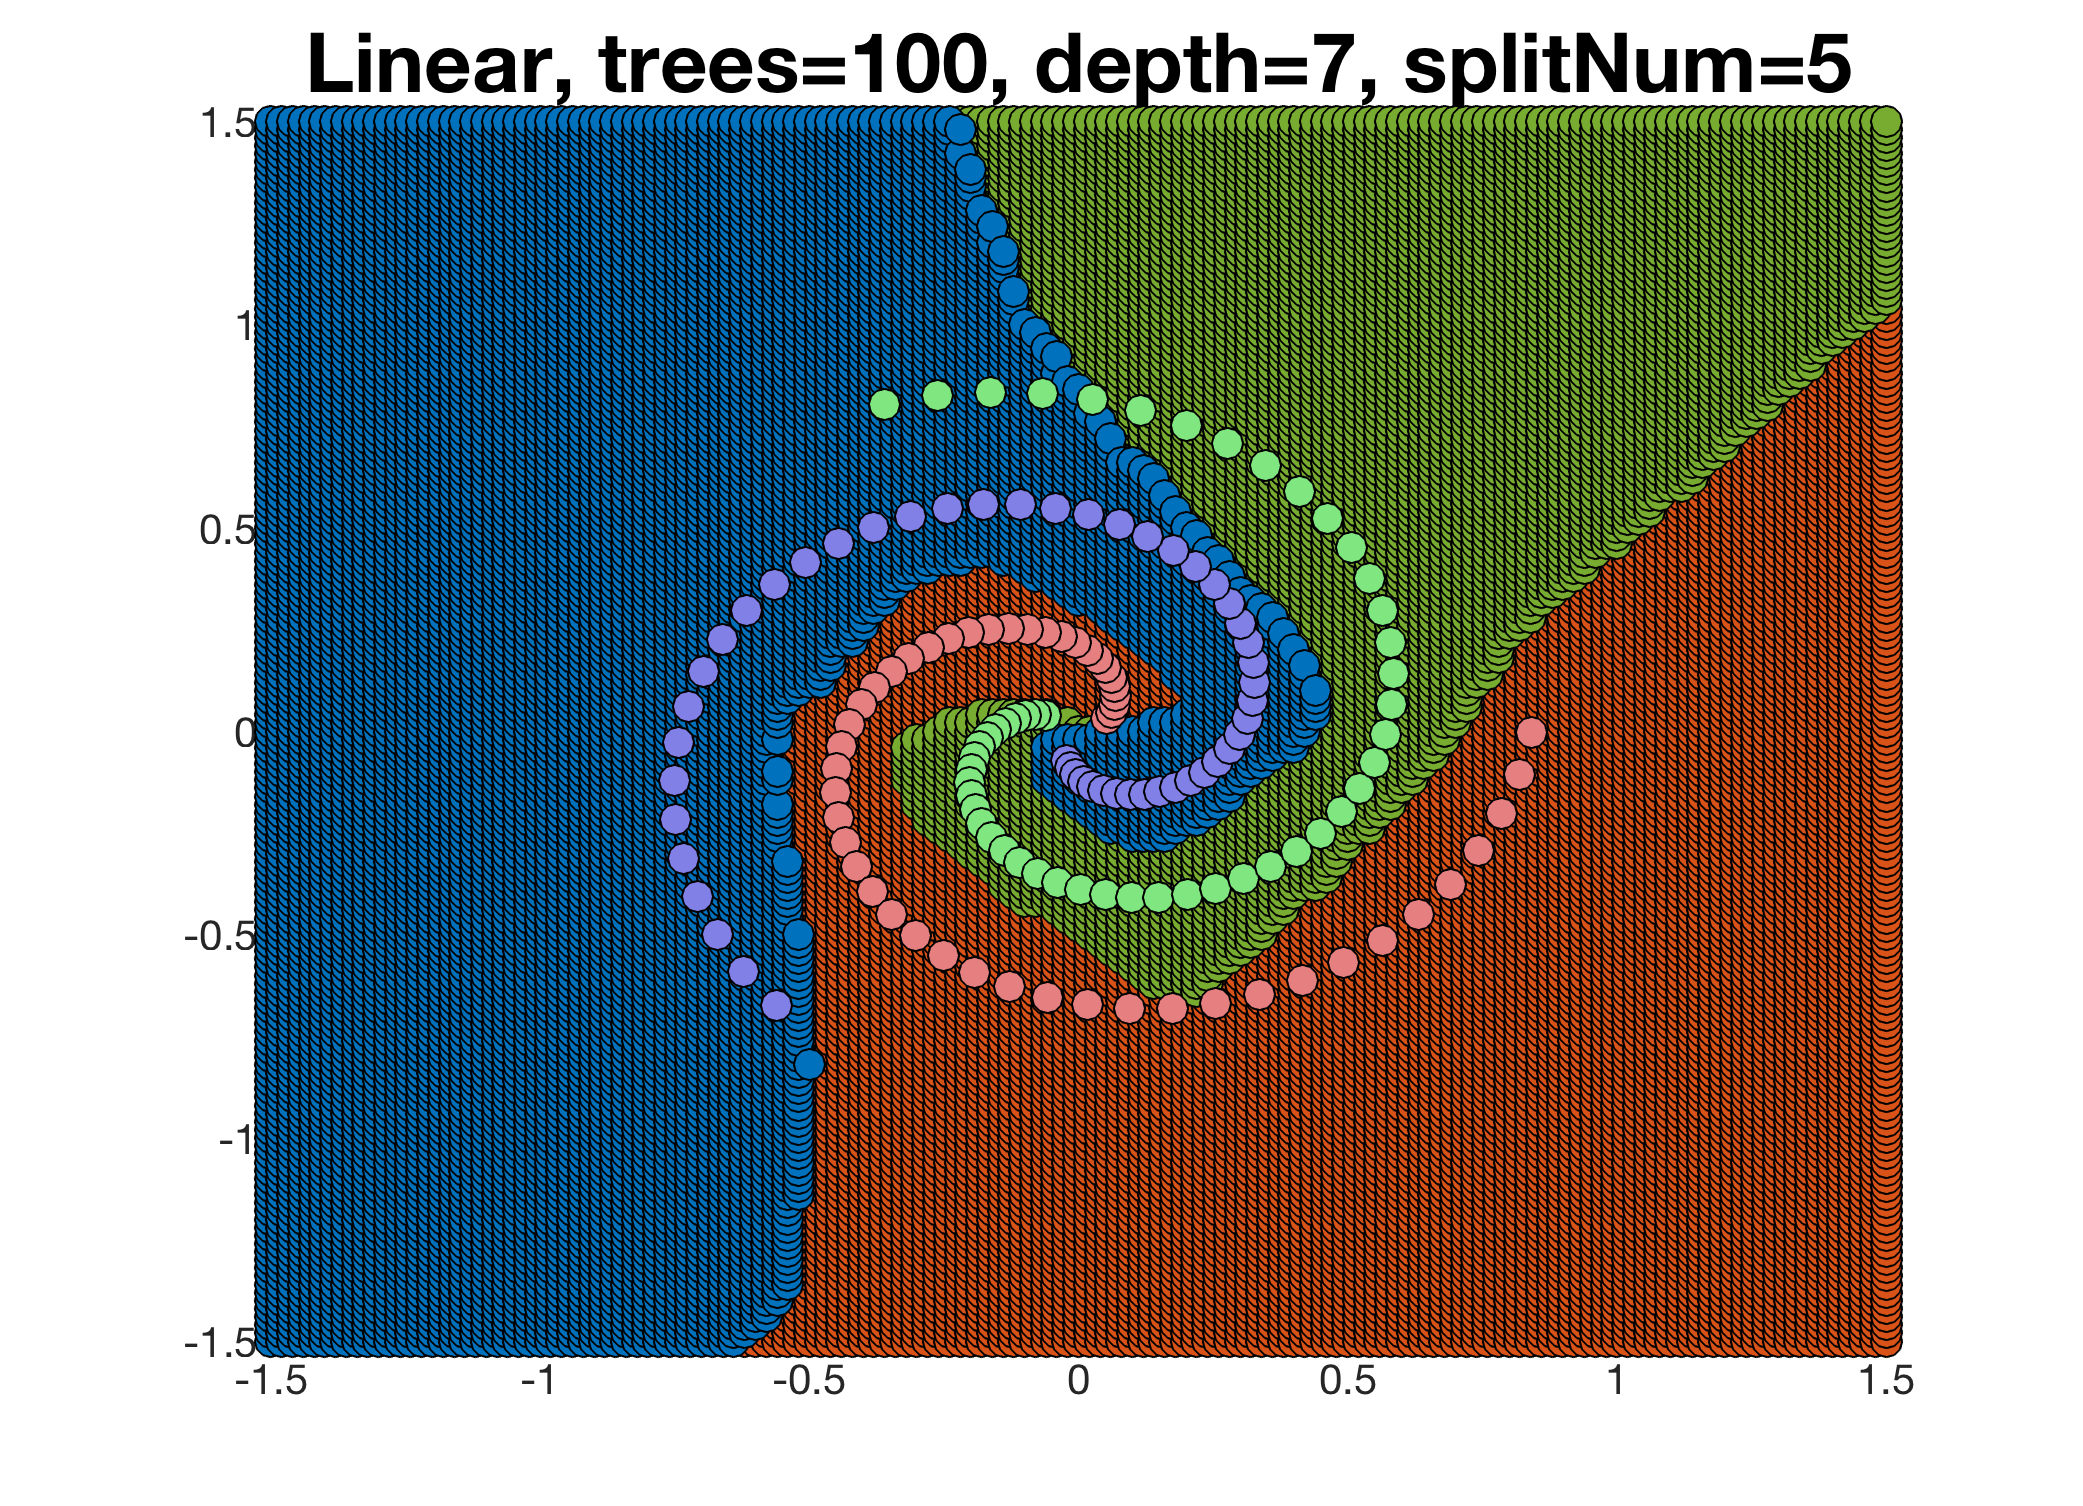
\includegraphics[width=0.40\columnwidth]{linear}
    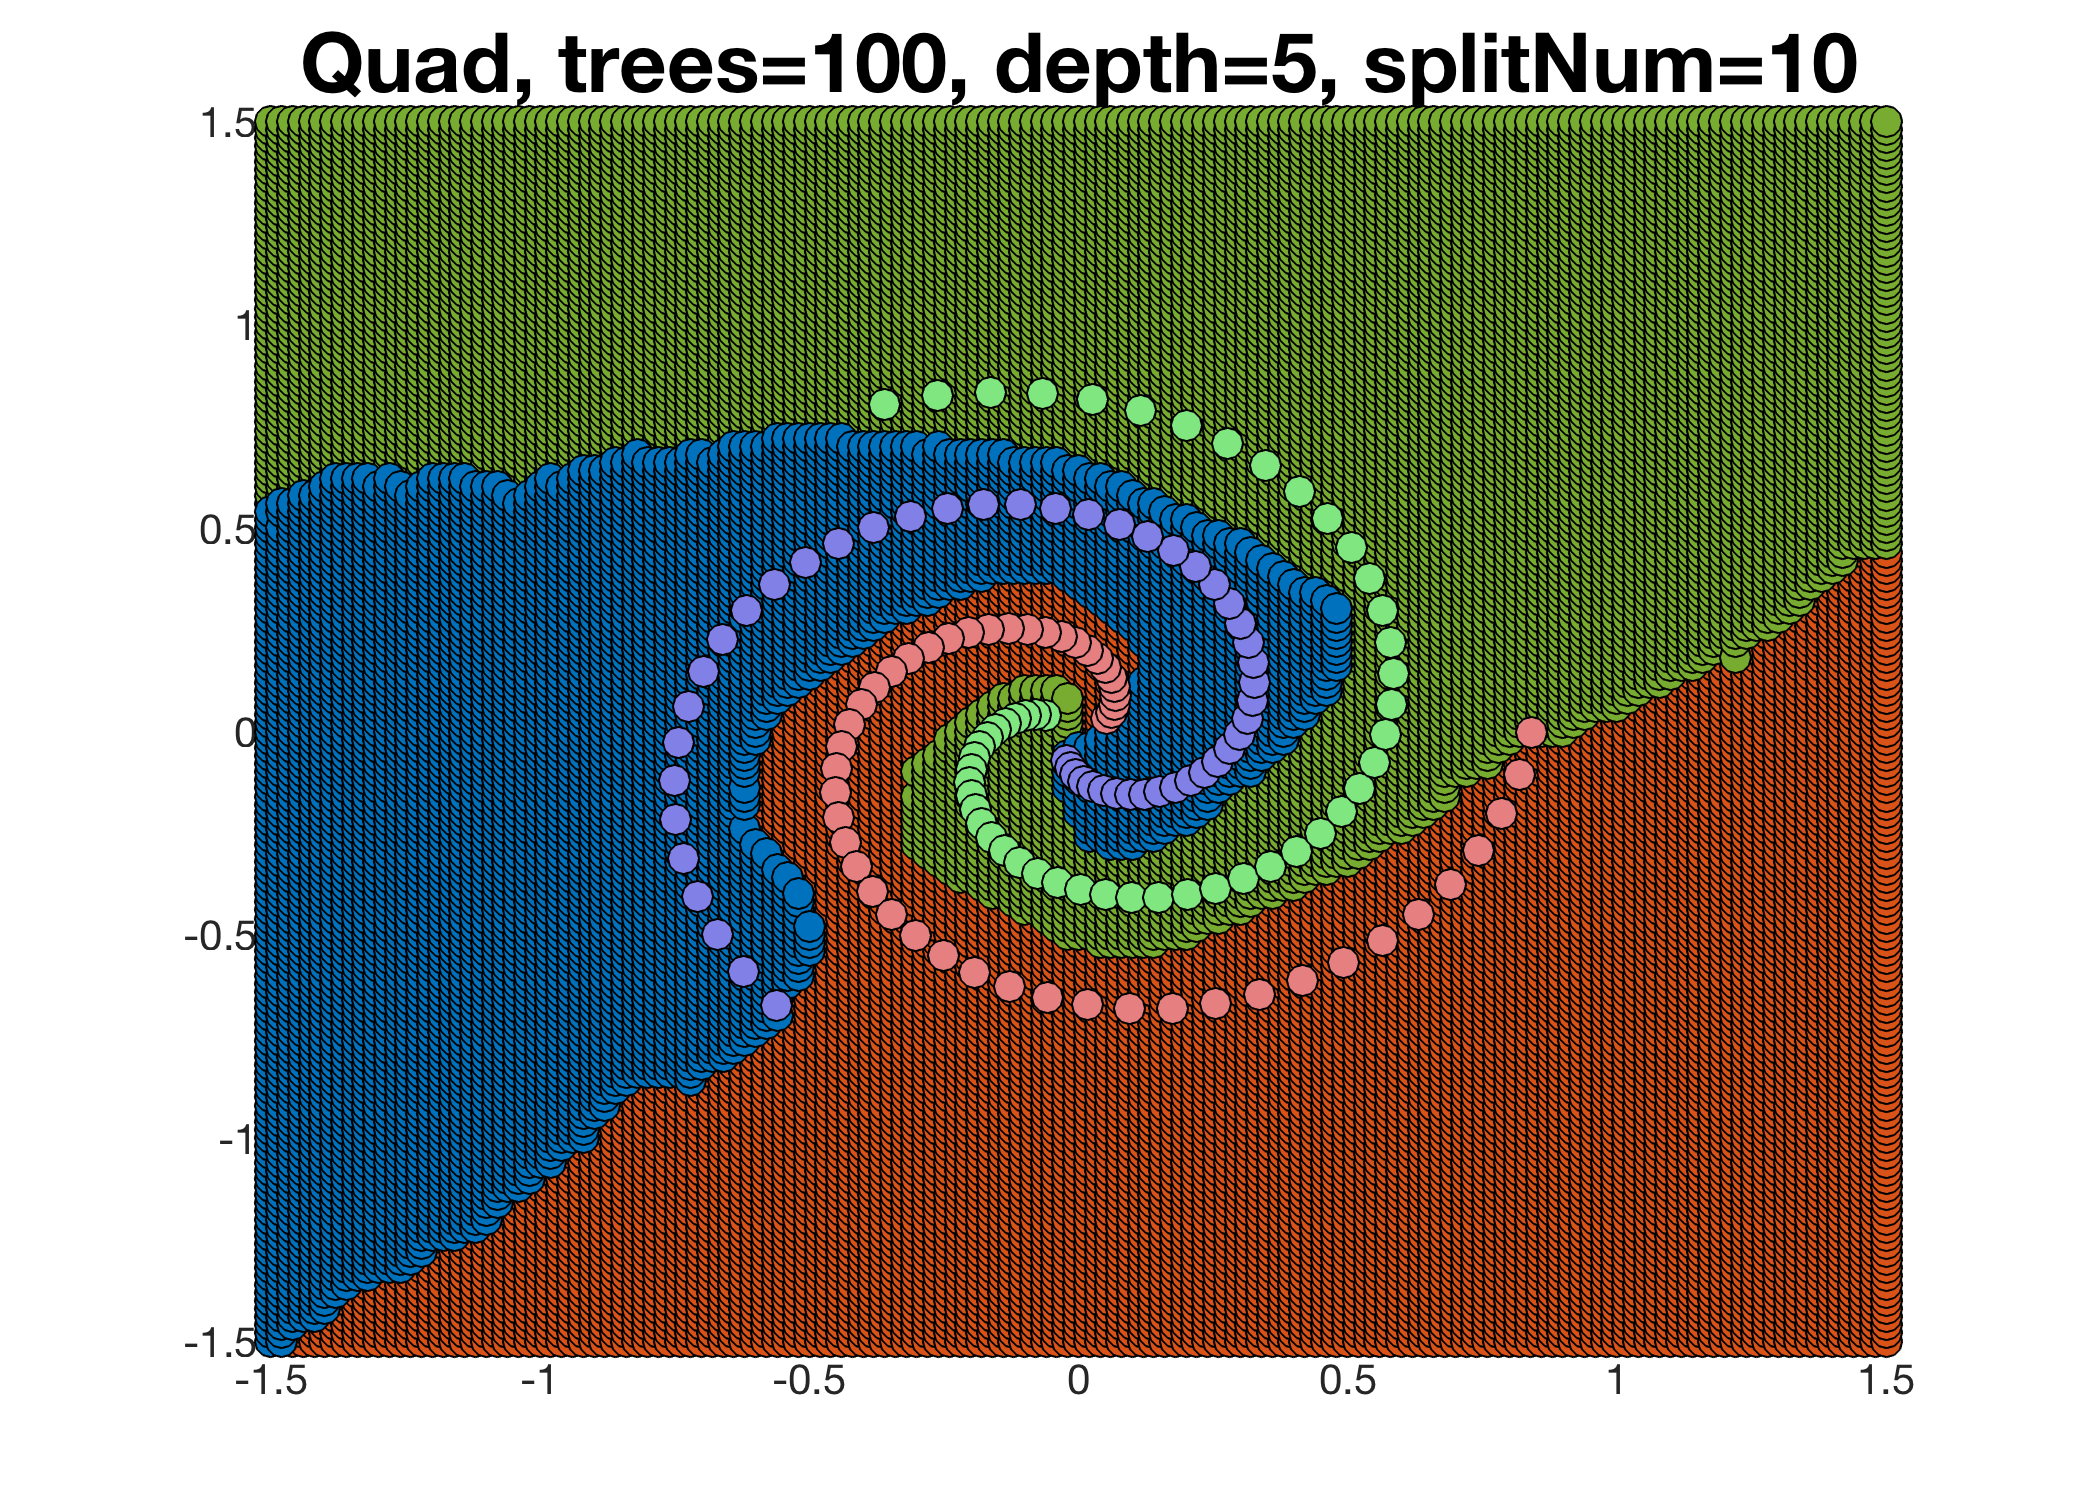
\includegraphics[width=0.40\columnwidth]{quad}
    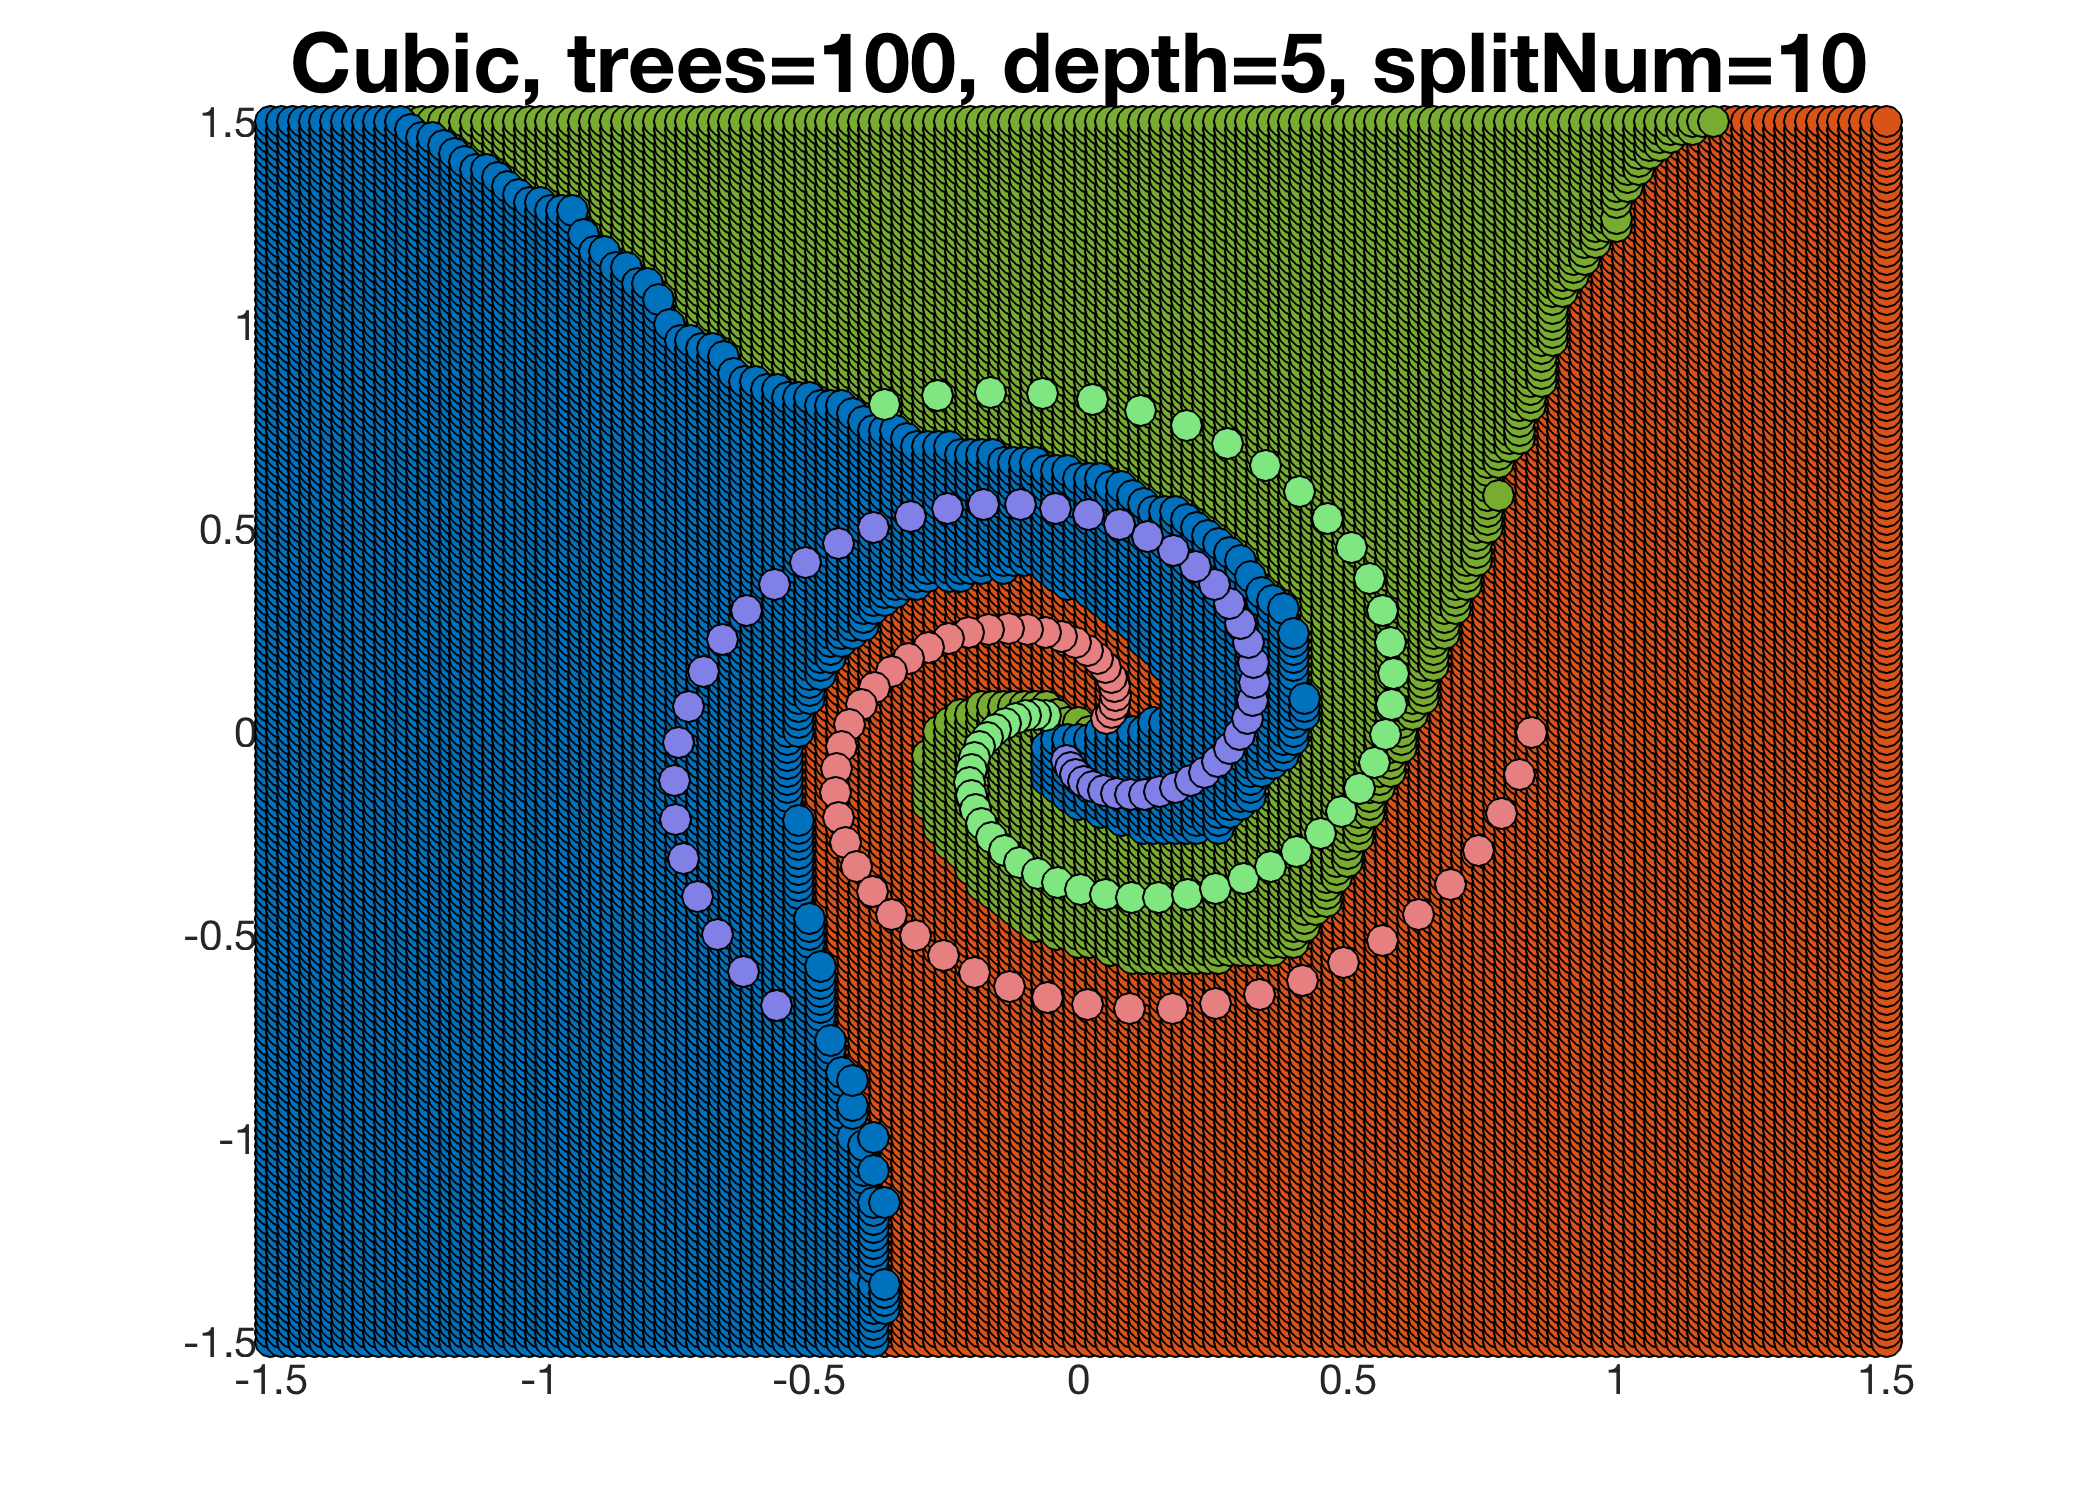
\includegraphics[width=0.40\columnwidth]{cubic}
    \caption{Overview of spectral subtraction process}
\end{figure}



\section{RF Classifier}

\begin{figure}[H]
	\centering
    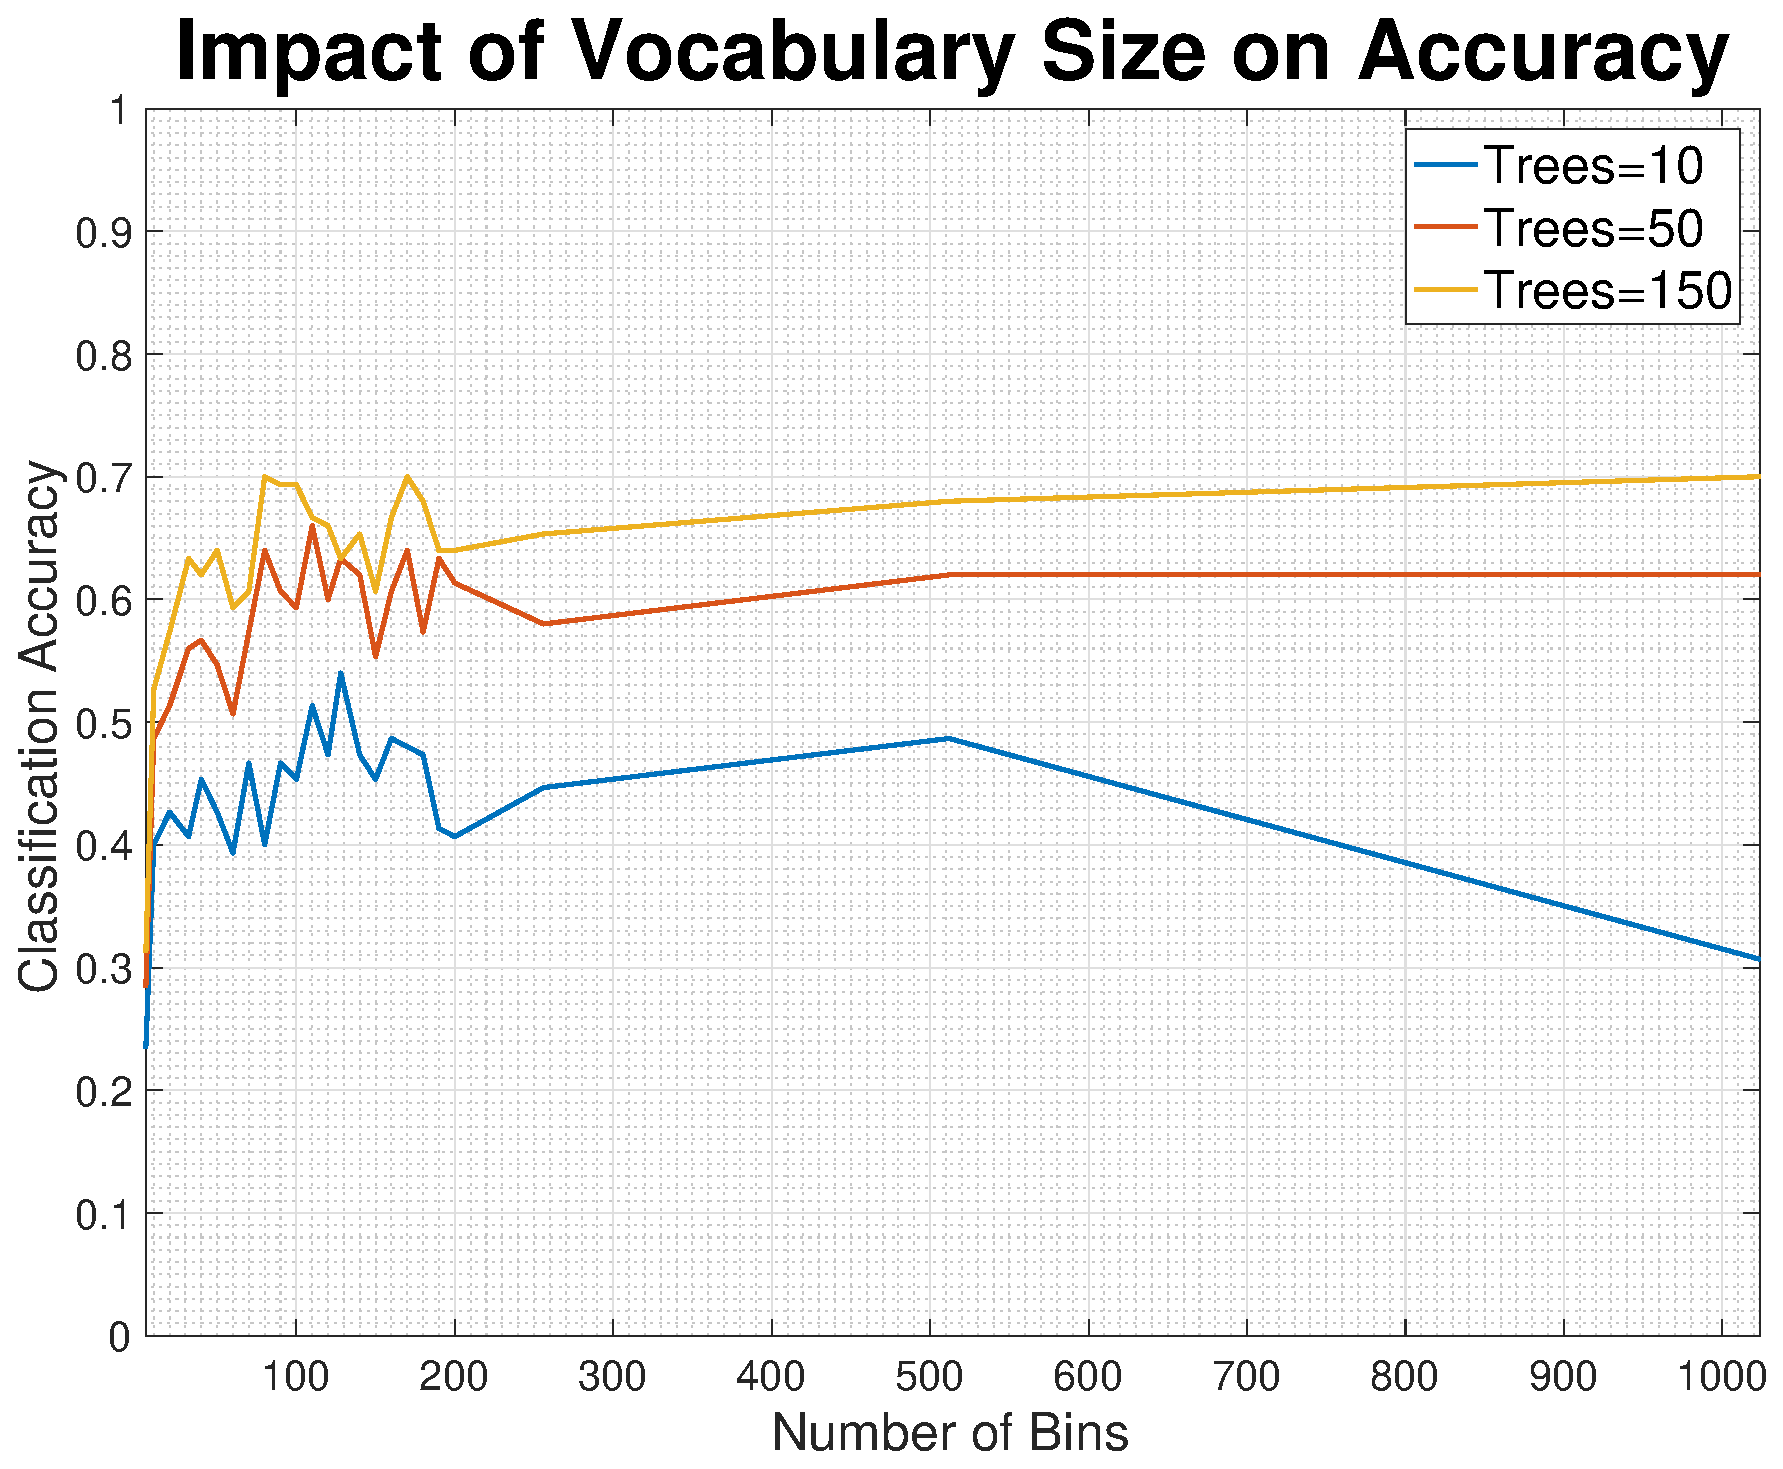
\includegraphics[width=0.49\columnwidth]{numBins_acc}
	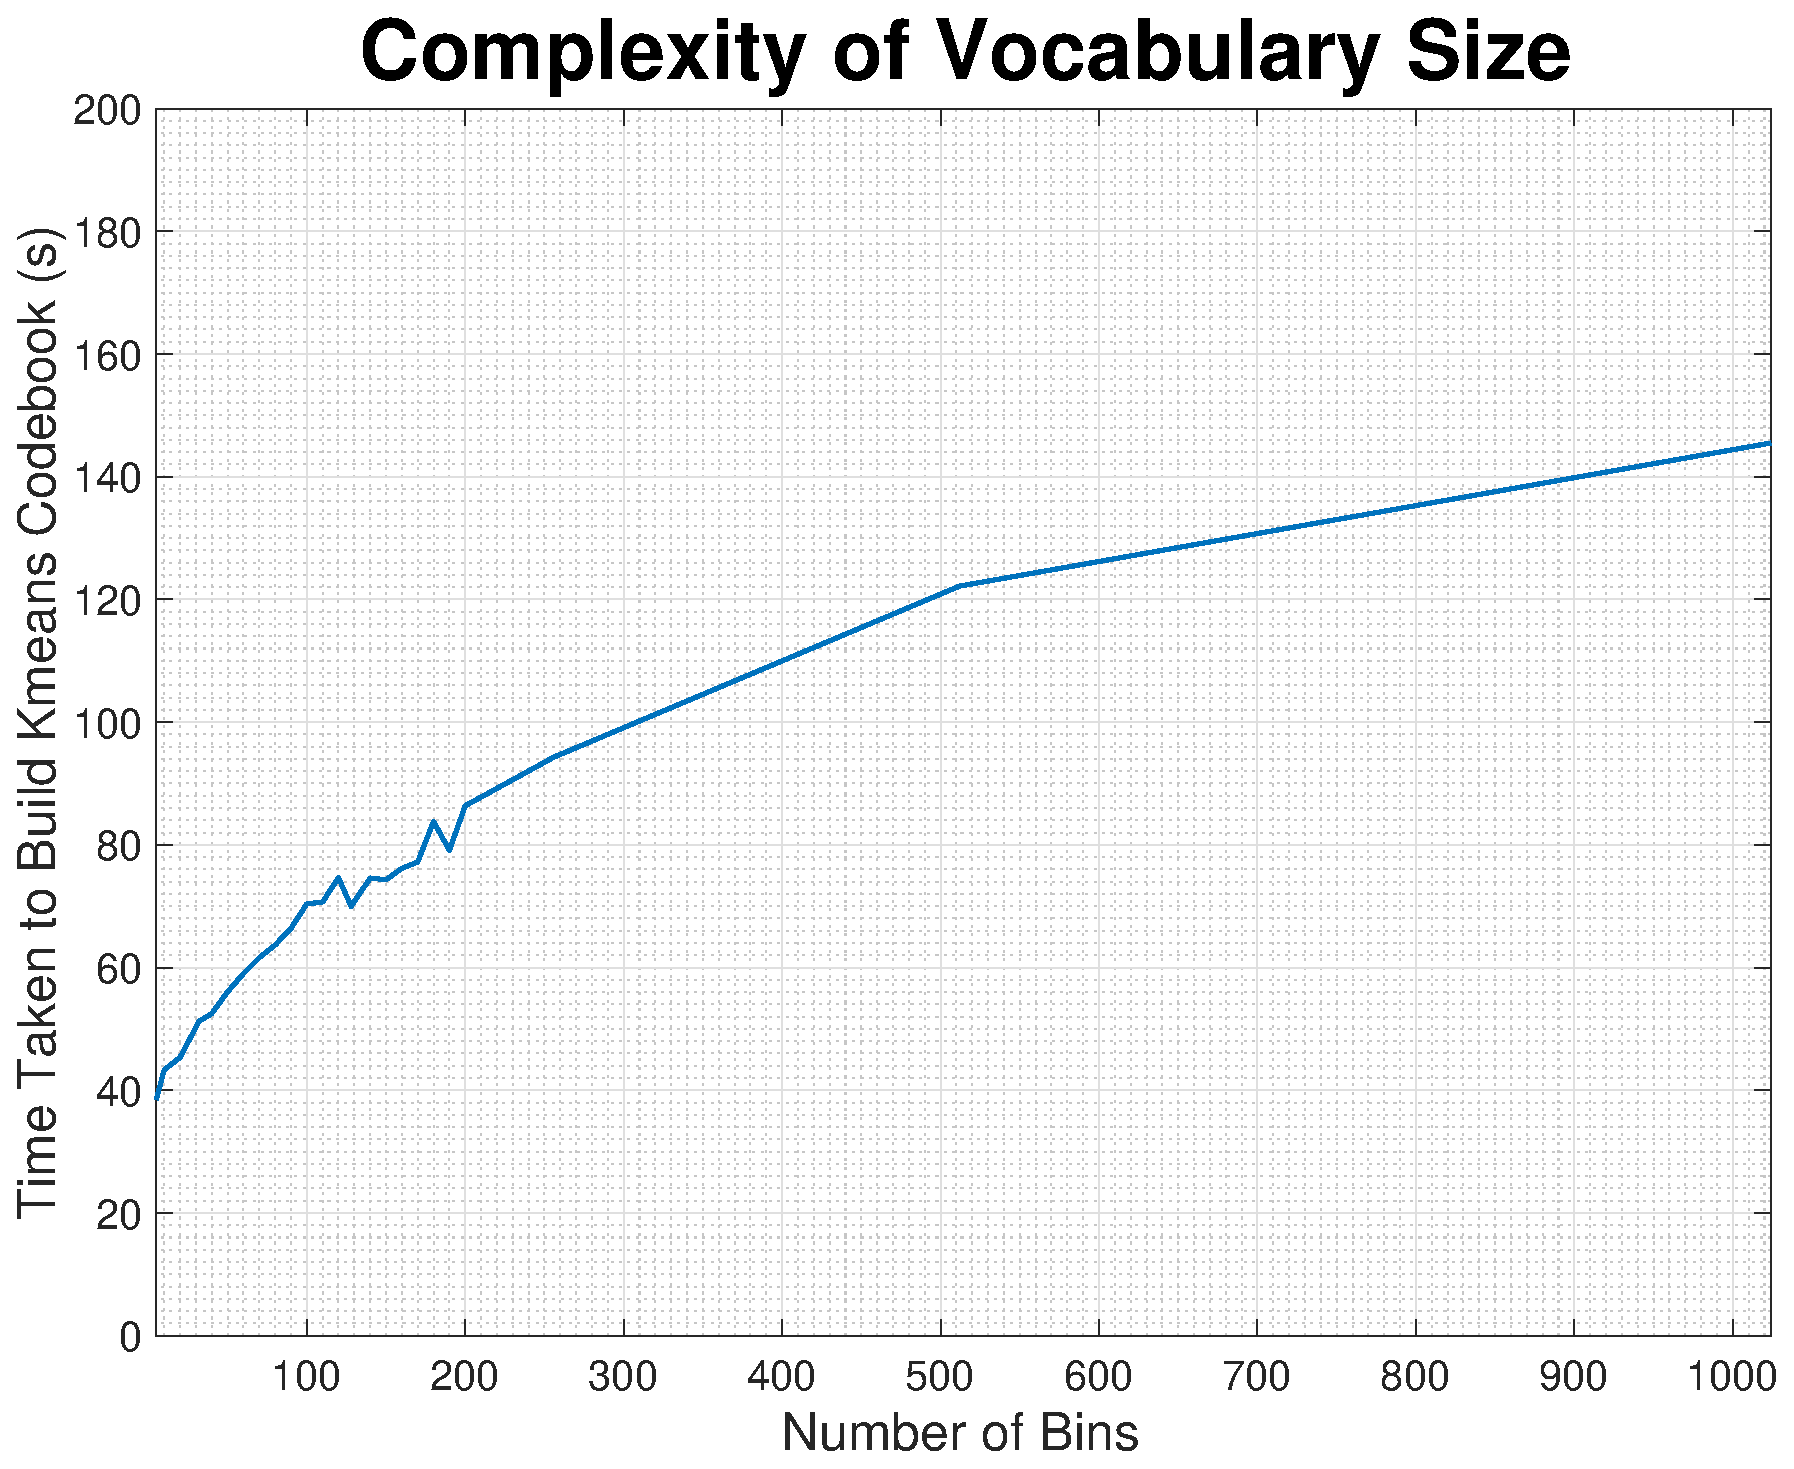
\includegraphics[width=0.49\columnwidth]{numBins_complexity}
    \caption{Overview of spectral subtraction process}
\end{figure}

\begin{figure}[H]
	\centering
    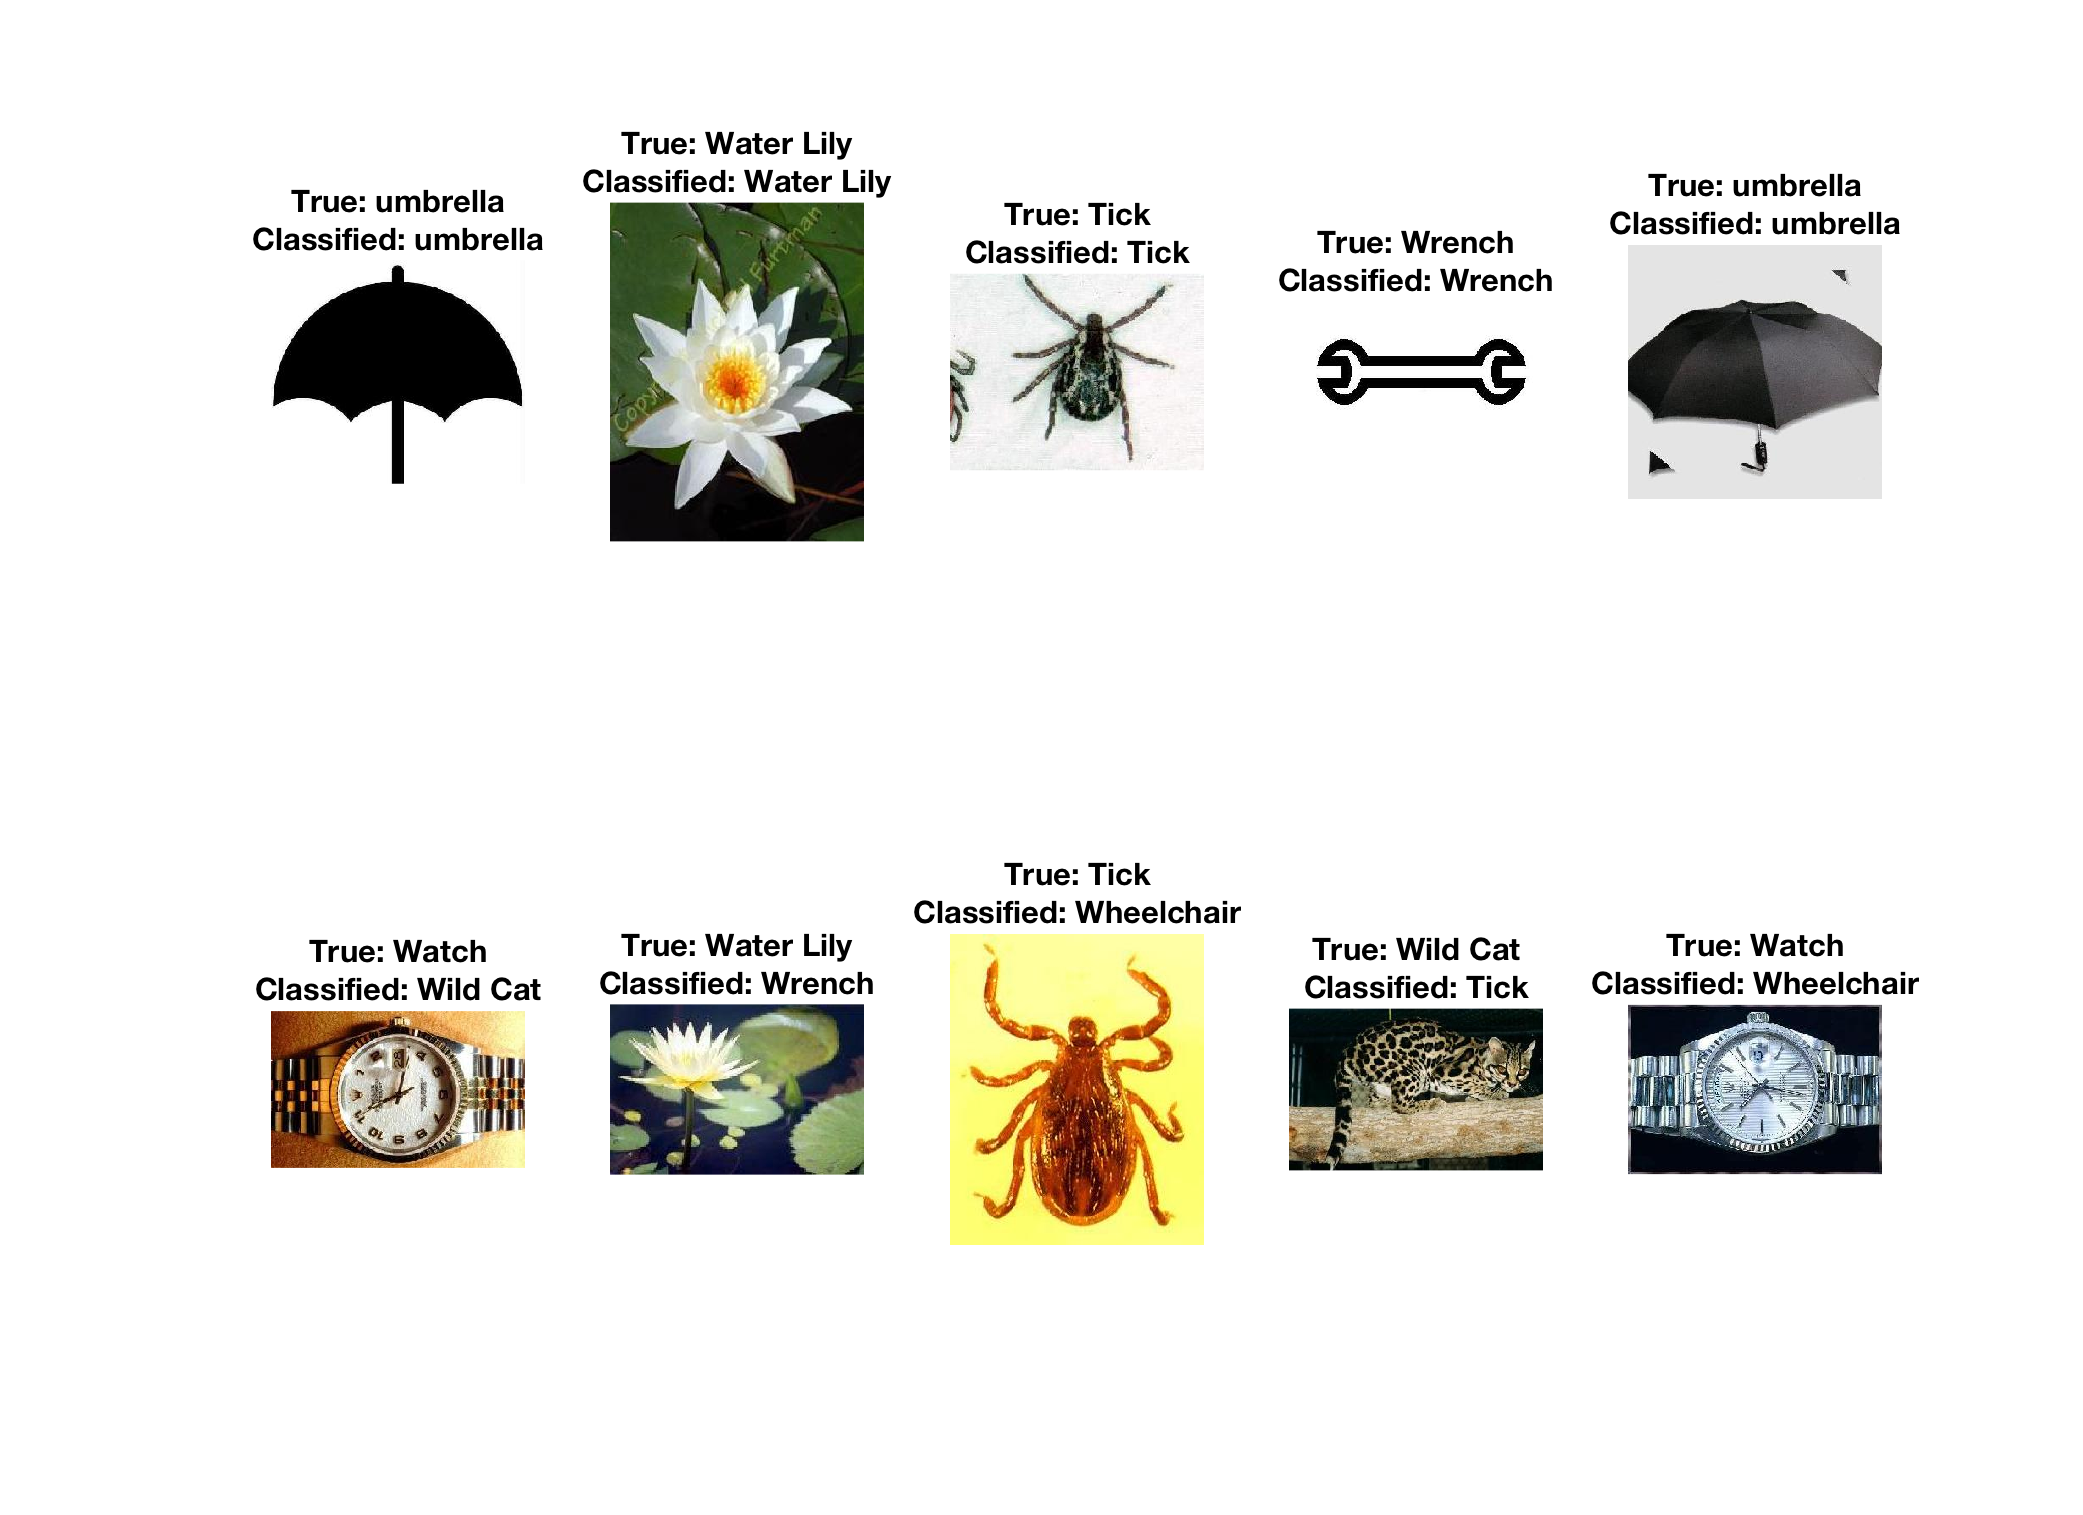
\includegraphics[width=0.60\columnwidth]{images}
    \caption{Overview of spectral subtraction process}
\end{figure}




\end{document}